\documentclass[]{book}
\usepackage{lmodern}
\usepackage{amssymb,amsmath}
\usepackage{ifxetex,ifluatex}
\usepackage{fixltx2e} % provides \textsubscript
\ifnum 0\ifxetex 1\fi\ifluatex 1\fi=0 % if pdftex
  \usepackage[T1]{fontenc}
  \usepackage[utf8]{inputenc}
\else % if luatex or xelatex
  \ifxetex
    \usepackage{mathspec}
  \else
    \usepackage{fontspec}
  \fi
  \defaultfontfeatures{Ligatures=TeX,Scale=MatchLowercase}
\fi
% use upquote if available, for straight quotes in verbatim environments
\IfFileExists{upquote.sty}{\usepackage{upquote}}{}
% use microtype if available
\IfFileExists{microtype.sty}{%
\usepackage{microtype}
\UseMicrotypeSet[protrusion]{basicmath} % disable protrusion for tt fonts
}{}
\usepackage[margin=1in]{geometry}
\usepackage{hyperref}
\PassOptionsToPackage{usenames,dvipsnames}{color} % color is loaded by hyperref
\hypersetup{unicode=true,
            pdftitle={Data Science avec R},
            pdfauthor={Fousseynou Bah},
            colorlinks=true,
            linkcolor=Maroon,
            citecolor=Blue,
            urlcolor=blue,
            breaklinks=true}
\urlstyle{same}  % don't use monospace font for urls
\usepackage{natbib}
\bibliographystyle{apalike}
\usepackage{color}
\usepackage{fancyvrb}
\newcommand{\VerbBar}{|}
\newcommand{\VERB}{\Verb[commandchars=\\\{\}]}
\DefineVerbatimEnvironment{Highlighting}{Verbatim}{commandchars=\\\{\}}
% Add ',fontsize=\small' for more characters per line
\usepackage{framed}
\definecolor{shadecolor}{RGB}{248,248,248}
\newenvironment{Shaded}{\begin{snugshade}}{\end{snugshade}}
\newcommand{\KeywordTok}[1]{\textcolor[rgb]{0.13,0.29,0.53}{\textbf{#1}}}
\newcommand{\DataTypeTok}[1]{\textcolor[rgb]{0.13,0.29,0.53}{#1}}
\newcommand{\DecValTok}[1]{\textcolor[rgb]{0.00,0.00,0.81}{#1}}
\newcommand{\BaseNTok}[1]{\textcolor[rgb]{0.00,0.00,0.81}{#1}}
\newcommand{\FloatTok}[1]{\textcolor[rgb]{0.00,0.00,0.81}{#1}}
\newcommand{\ConstantTok}[1]{\textcolor[rgb]{0.00,0.00,0.00}{#1}}
\newcommand{\CharTok}[1]{\textcolor[rgb]{0.31,0.60,0.02}{#1}}
\newcommand{\SpecialCharTok}[1]{\textcolor[rgb]{0.00,0.00,0.00}{#1}}
\newcommand{\StringTok}[1]{\textcolor[rgb]{0.31,0.60,0.02}{#1}}
\newcommand{\VerbatimStringTok}[1]{\textcolor[rgb]{0.31,0.60,0.02}{#1}}
\newcommand{\SpecialStringTok}[1]{\textcolor[rgb]{0.31,0.60,0.02}{#1}}
\newcommand{\ImportTok}[1]{#1}
\newcommand{\CommentTok}[1]{\textcolor[rgb]{0.56,0.35,0.01}{\textit{#1}}}
\newcommand{\DocumentationTok}[1]{\textcolor[rgb]{0.56,0.35,0.01}{\textbf{\textit{#1}}}}
\newcommand{\AnnotationTok}[1]{\textcolor[rgb]{0.56,0.35,0.01}{\textbf{\textit{#1}}}}
\newcommand{\CommentVarTok}[1]{\textcolor[rgb]{0.56,0.35,0.01}{\textbf{\textit{#1}}}}
\newcommand{\OtherTok}[1]{\textcolor[rgb]{0.56,0.35,0.01}{#1}}
\newcommand{\FunctionTok}[1]{\textcolor[rgb]{0.00,0.00,0.00}{#1}}
\newcommand{\VariableTok}[1]{\textcolor[rgb]{0.00,0.00,0.00}{#1}}
\newcommand{\ControlFlowTok}[1]{\textcolor[rgb]{0.13,0.29,0.53}{\textbf{#1}}}
\newcommand{\OperatorTok}[1]{\textcolor[rgb]{0.81,0.36,0.00}{\textbf{#1}}}
\newcommand{\BuiltInTok}[1]{#1}
\newcommand{\ExtensionTok}[1]{#1}
\newcommand{\PreprocessorTok}[1]{\textcolor[rgb]{0.56,0.35,0.01}{\textit{#1}}}
\newcommand{\AttributeTok}[1]{\textcolor[rgb]{0.77,0.63,0.00}{#1}}
\newcommand{\RegionMarkerTok}[1]{#1}
\newcommand{\InformationTok}[1]{\textcolor[rgb]{0.56,0.35,0.01}{\textbf{\textit{#1}}}}
\newcommand{\WarningTok}[1]{\textcolor[rgb]{0.56,0.35,0.01}{\textbf{\textit{#1}}}}
\newcommand{\AlertTok}[1]{\textcolor[rgb]{0.94,0.16,0.16}{#1}}
\newcommand{\ErrorTok}[1]{\textcolor[rgb]{0.64,0.00,0.00}{\textbf{#1}}}
\newcommand{\NormalTok}[1]{#1}
\usepackage{longtable,booktabs}
\usepackage{graphicx,grffile}
\makeatletter
\def\maxwidth{\ifdim\Gin@nat@width>\linewidth\linewidth\else\Gin@nat@width\fi}
\def\maxheight{\ifdim\Gin@nat@height>\textheight\textheight\else\Gin@nat@height\fi}
\makeatother
% Scale images if necessary, so that they will not overflow the page
% margins by default, and it is still possible to overwrite the defaults
% using explicit options in \includegraphics[width, height, ...]{}
\setkeys{Gin}{width=\maxwidth,height=\maxheight,keepaspectratio}
\IfFileExists{parskip.sty}{%
\usepackage{parskip}
}{% else
\setlength{\parindent}{0pt}
\setlength{\parskip}{6pt plus 2pt minus 1pt}
}
\setlength{\emergencystretch}{3em}  % prevent overfull lines
\providecommand{\tightlist}{%
  \setlength{\itemsep}{0pt}\setlength{\parskip}{0pt}}
\setcounter{secnumdepth}{5}
% Redefines (sub)paragraphs to behave more like sections
\ifx\paragraph\undefined\else
\let\oldparagraph\paragraph
\renewcommand{\paragraph}[1]{\oldparagraph{#1}\mbox{}}
\fi
\ifx\subparagraph\undefined\else
\let\oldsubparagraph\subparagraph
\renewcommand{\subparagraph}[1]{\oldsubparagraph{#1}\mbox{}}
\fi

%%% Use protect on footnotes to avoid problems with footnotes in titles
\let\rmarkdownfootnote\footnote%
\def\footnote{\protect\rmarkdownfootnote}

%%% Change title format to be more compact
\usepackage{titling}

% Create subtitle command for use in maketitle
\newcommand{\subtitle}[1]{
  \posttitle{
    \begin{center}\large#1\end{center}
    }
}

\setlength{\droptitle}{-2em}

  \title{Data Science avec R}
    \pretitle{\vspace{\droptitle}\centering\huge}
  \posttitle{\par}
    \author{Fousseynou Bah}
    \preauthor{\centering\large\emph}
  \postauthor{\par}
      \predate{\centering\large\emph}
  \postdate{\par}
    \date{2019-03-05}

\usepackage{booktabs}

\begin{document}
\maketitle

{
\hypersetup{linkcolor=black}
\setcounter{tocdepth}{1}
\tableofcontents
}
\chapter{Introduction}\label{introduction}

\section{\texorpdfstring{Un autre livre sur la \emph{data science}!
Vraiment?}{Un autre livre sur la data science! Vraiment?}}\label{un-autre-livre-sur-la-data-science-vraiment}

En décidant d'écrire un livre sur la \emph{data science}, j'ai
longuement débattu dans ma propre tête, je me suis posé plusieurs
questions dont une qui revenait constamment: ``a-t-on vraiment besoin
d'un autre livre sur la \emph{data science}?'' ``N'en-t-on pas assez?''
Avec le succès dont jouit la discipline, ce n'est certainement pas les
ressources qui manquent, aussi bien en ligne que dans les librairies. Et
surtout, je me demandais bien ``qu'avais-je à dire qui n'avait pas été
dit''? Et pourtant, quelques raisons m'ont poussé à reconsidérer ma
position.

La première est assez égoïte. On n'apprend jamais aussi bien qu'en
enseignant. Pour m'assurer que j'avais bien assimilé les connaissances
que j'avais acquises dans ce domaine, il n'y avait rien de mieux que de
me livrer à un exercice de pédagogue. Expliquer à d'autres ce que
j'avais appris. N'est-ce pas là que réside l'ultime test pour un
apprenant! C'est partant de cette idée que je me suis mis à faire des
diapositives dans le cadre des mes enseignements. Très tôt, j'ai réalisé
que les diapositives ne sauraient jouer leur rôle, qui est d'offrir un
aperçu synthétique d'une idée développée par un narrateur, et satifaire
l'apprenant qui souhaiterai obtenir des explications détaillées. Ce
travail revient au narrateur, à défaut de qui l'on se tourne vers un
manuel. Donc, il me fallait bien accompagner les diapositives d'un
support plus détaillé pour mieux outiller mes étudiants.

La seconde raison est le contexte. Malgré l'abondance et la qualité des
ressources disponibles sur la \emph{data science} et malgré l'accès de
plus en plus facile - coût faible et gratuité pour beaucoup -, il
demeure que l'étudiant africain peut souvent se sentir éloigné du
contexte à travers lequel la \emph{data science} est présentée. Or,
cell-ci est avant tout une discipline de contexte. Bien que mélangeant
informatique, mathématiques, statistiques\ldots{}et bien d'autres
expertises, elle est avant tout un outil, mobilisée pour répondre à des
questions. Et ces questions sont très contextuelles. Il ne fait aucun
doute que le disponibilité et l'accéssibilité des données sur le monde
industrialisé rend leur utilisation commode pour introduire la
\emph{data science} à un jeune africain est très commode. Mais la
distance entre le contexte présenté et celui qui est vécu par le
bénéficiaire pose un problème. Elle empêche l'appropriation de la
discipline. De ce fait, je me suis trouvé dans ce constat une raison de
m'engager dans ce projet et surtout de me forcer à utiliser des données
sur le contexte local. Après tout, l'être humain n'est-il pas plus
enclin à vous prêter attention quand vous lui parlez de lui-même?

\section{\texorpdfstring{La \emph{data
science}}{La data science}}\label{la-data-science}

Comme toute discipline qui connaît une expansion rapide, il est
difficile de définir la \emph{data science}. Elle est vaste et riche,
tant de par les disciplines dont elle emprunte des morceaux pour se
contituer en entité que de par les branches qu'elle pousse avec sa
propre croissance.

Commençons par quelques exemples

Fait de la \emph{data science}:

\begin{itemize}
\item
  l'économiste qui examine le niveau du PIB sur 30 ans et cherche à
  dégager des scénarii pour des futures évolutions;
\item
  le sociologue qui s'appuie le taux de natalité et le taux de
  participation des femmes au marché du travail pour comprendre
  l'évolution de la place de la femme dans la société;
\item
  le météorologue qui cherche à prédire la pluviométrie de la semaine à
  venir en modélisant les données historiques;
\item
  l'épidémiologue qui cartographie le taux de prévalence du paludisme
  pour appuyer un programme stratégique;
\item
  etc.
\end{itemize}

Le caractère transversale de la \emph{data science} apparait ici quand
on sait que ces individus sont de disciplines différentes et poursuivent
des questions tout aussi distantes les unes des autres. Et pourtant, les
données les réunissent tous. Ils ont chacun besoin de trouver dans
celles-ci un appui pour améliorer leur propre compréhension du phénomène
étudié, tester leurs hypothèses, fonder leurs recommandations ou
même\ldots{}reconforter leurs propres idées ou mieux s'armer pour
rejetter celles de leurs adversaires (les données ne sont aussi neutres
que celui qui les manipule!)

Selon
\href{https://en.wikipedia.org/wiki/Data_science}{\textcolor{blue}{Wikipédia}},
la \emph{data science} est un champ interdisciplinaire qui utilise les
méthode, processus, algorithmes et systèmes scientifiques pour extraire
des données - tant structurées que non structurées - des informations
utiles à la compréhension et à la prise de décision. De ce fait, elle
s'appuie sur diverses méthodes (mathématiques, statistiques,
informatiques, etc.) pour tirer des données une compréhension meilleure
de phénomènes d'intérêt.

\section{\texorpdfstring{Le \emph{data
scientist}}{Le data scientist}}\label{le-data-scientist}

Et le \emph{data scientist} dans tout ça? Il est apparait désormais
comme la perle rare. Un individu capable de parler aux hommes, aux
machines et aux données. Aux:

\begin{itemize}
\item
  hommes, il pose les questions auxquelles il a la charge d'offrir des
  réponses.
\item
  machines, il parle à travers des langages spécifiques (R, Python,
  Julia,\ldots{}), des langages qui ressemblent à bien d'égards à ceux
  avec lesquels il s'entretient avec les humains car ils sont basés sur
  des règles précises et sont vivants et évolutifs;
\item
  données, il applique des méthodes d'investigation où l'expérience,
  l'intuition, le sens artistique interviennent tout autant que la
  connaissance du domaine d'intervention. Dans les données disponibles,
  il cherche à séparer les bonnes des mauvaises, les utiles des
  nuisibles. A celles qu'il sélectionne, il cherche le bon format, la
  bonne structure. Sur celles qu'il retient, il teste des modèles, sans
  oublier la place importante de la visualisation à tous les niveaux.
  Bref, un vrai détective!
\end{itemize}

Face à la génération massive des données, le besoin de \emph{data
scientist} se fait pressant partout. De ce fait l'engouement ne manque
pas pour les jeunes désireux de se lancer. Mais le portrait de
super-homme généralement fait du \emph{data scientist} (ne cherchez pas
plus loin que les lignes d'en dessus!), l'on peut croire qu'il faut être
spécial pour embrasser la profession. Du tout! Celà dit, certaines
compétences sont utiles.

Alors, qu'est-ce qu'il faut pour être \emph{data scientist}?

\begin{itemize}
\item
  pas nécéssairement un diplôme avancé en mathématiques ou en
  statistiques\ldots{}quoiqu'il est utile de maîtriser des concepts de
  bases (les concepts algébriques comme le vecteur, la matrice,\ldots{}
  et les notions statistiques comme la moyenne, l'écart-type, etc.);
\item
  pas forcément un diplôme en informatique ou en
  programmation\ldots{}quoiqu'il est utile de connaître les notions de
  bases (qu'est-ce qu'un objet, un environnement? quels types d'objets
  peut-on manipuler dans un environnement donnée\ldots{}?);
\item
  une connaissance avérée dans un domaine spécifique dans lequel l'on
  peut soulever des questions, mobiliser des outils théoriques auxquels
  on confronte les résultats de l'analyse conduite sur les données;
\item
  un esprit curieux, quelle que soit l'avenue que l'on emprunte.
\end{itemize}

Vous pourrez avoir une meilleure idée en surfant sur le net (Google est
votre ami!)

\section{R}\label{r}

\subsection{Qu'est-ce que c'est que R?}\label{quest-ce-que-cest-que-r}

Voici basiquement ce que
\href{https://fr.wikipedia.org/wiki/R_(langage)}{Wikipédia} dit.
\href{http://r-project.org}{\textcolor{blue}{R}} est un langage de
programmation et un logiciel gratuit et libre. Il est surtout utilisé
pour le développement de programmes statistiques et des analyses de
données. Il gagne en popularité depuis quelques années avec l'émergence
de la \emph{data science} et du fait qu'il est gratuit et ouvert
(\emph{open-source}). R est née d'un projet de recherche mené par deux
chercheurs, Ross Ihaka et Robert Gentleman à l'université d'Auckland
(Nouvelle-Zélande) en 1993. En 1997 est mis en place le
\emph{Comprehension R Archive Network (CRAN)} qui centralise les
contributions au projet

Depuis le projet connaît une croissance soutenue, grâce à des
contributions de la part de milliers de personnes à travers le monde.

\subsection{Pourquoi R?}\label{pourquoi-r}

Pour un apprenti \emph{data scientist}, le choix du langage et/ou du
programme est une décision critique. Considérant le temps qu'il
investira en apprentissage et le retour qu'il espéra à travers
l'utilisation de ses nouvelles connaissances dans sa profession, il est
utile de considerer divers critères dont:

\begin{itemize}
\item
  l'accessibilité de l'outil en termes de coûts: tous les langages de
  programmation ne sont pas gratuits comme R! Certains
  coûtent\ldots{}chers mêmes ;
\item
  l'accessibilité du langage en termes de syntaxe: R est très
  compréhensible (surtout pour quelqu'un qui se retrouve un peu avec la
  langue anglaise);
\item
  la popularité du langage parmi les paires: tout le monde s'est mis à
  l'anglais, même dans les pays où ce n'est pas la langue dominante.
  N'est-ce pas? De la même façon, il est important pour le \emph{data
  scientist} d'embrasser un langage qui est aussi utilisé par ceux avec
  lesquels il sera amené à collaborer. A ce niveau, R est très
  populaire.
\item
  la dynamique de développement du langage: le langage étant un
  investissement en soit, il est important de miser sur ceux qui
  présentent un avenir. Et ceux-ci sont ceux qui mutent avec la
  technologie et les besoins des utilisateurs. A ce niveau encore, R
  présente des arguments. Il dispose du réseau \emph{CRAN} alimenté par
  des milliers de contributeurs, divers aussi bien de par leur position
  dans le monde que de par leur discipline.
\end{itemize}

\subsection{R dans l'écosystème des
langages}\label{r-dans-lecosysteme-des-langages}

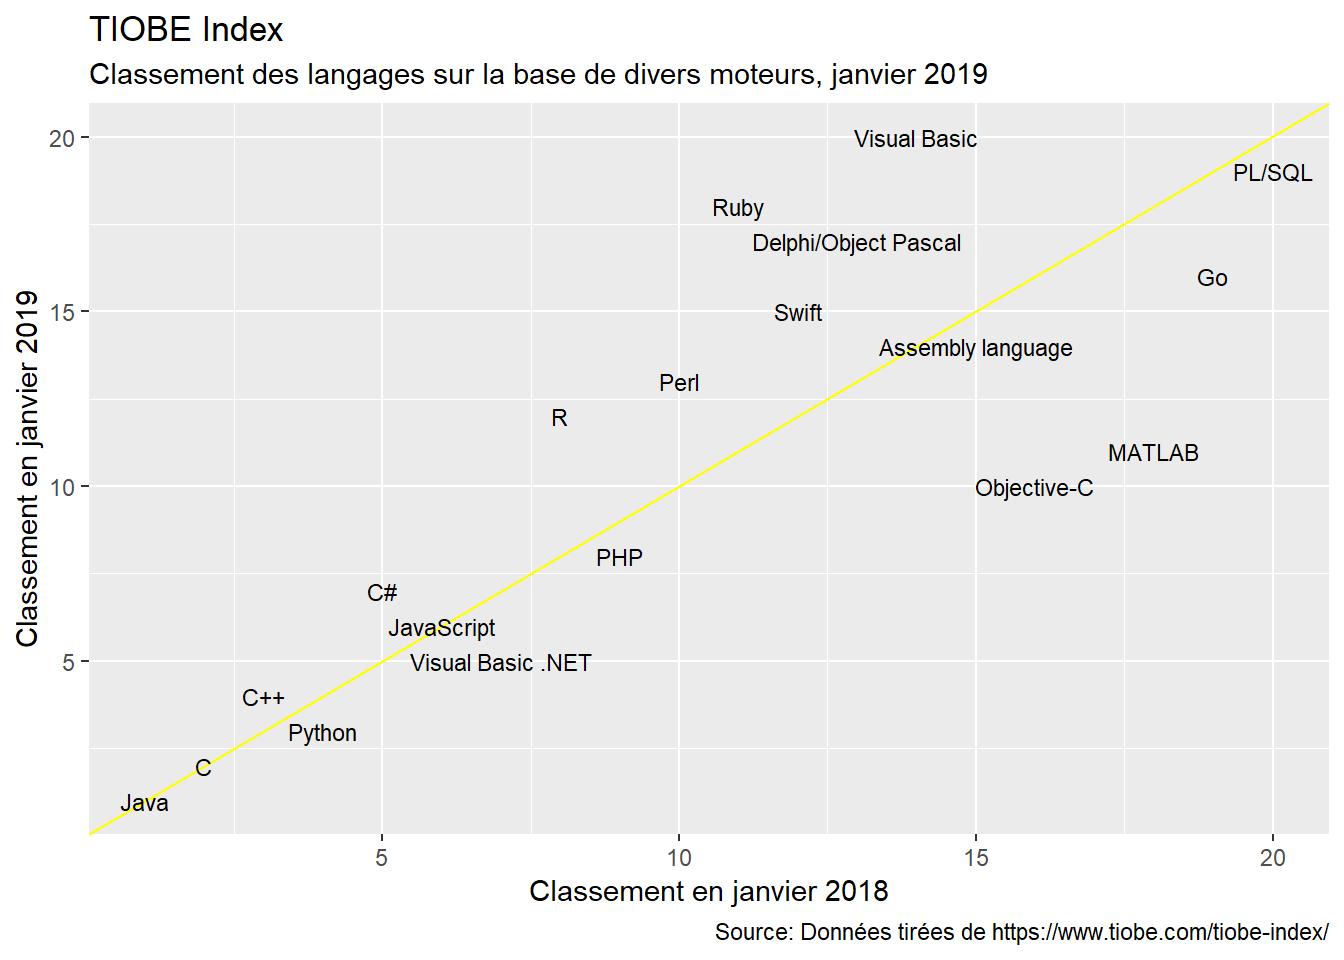
\includegraphics[width=1\linewidth,height=1\textheight]{dswr_book_files/figure-latex/unnamed-chunk-3-1}

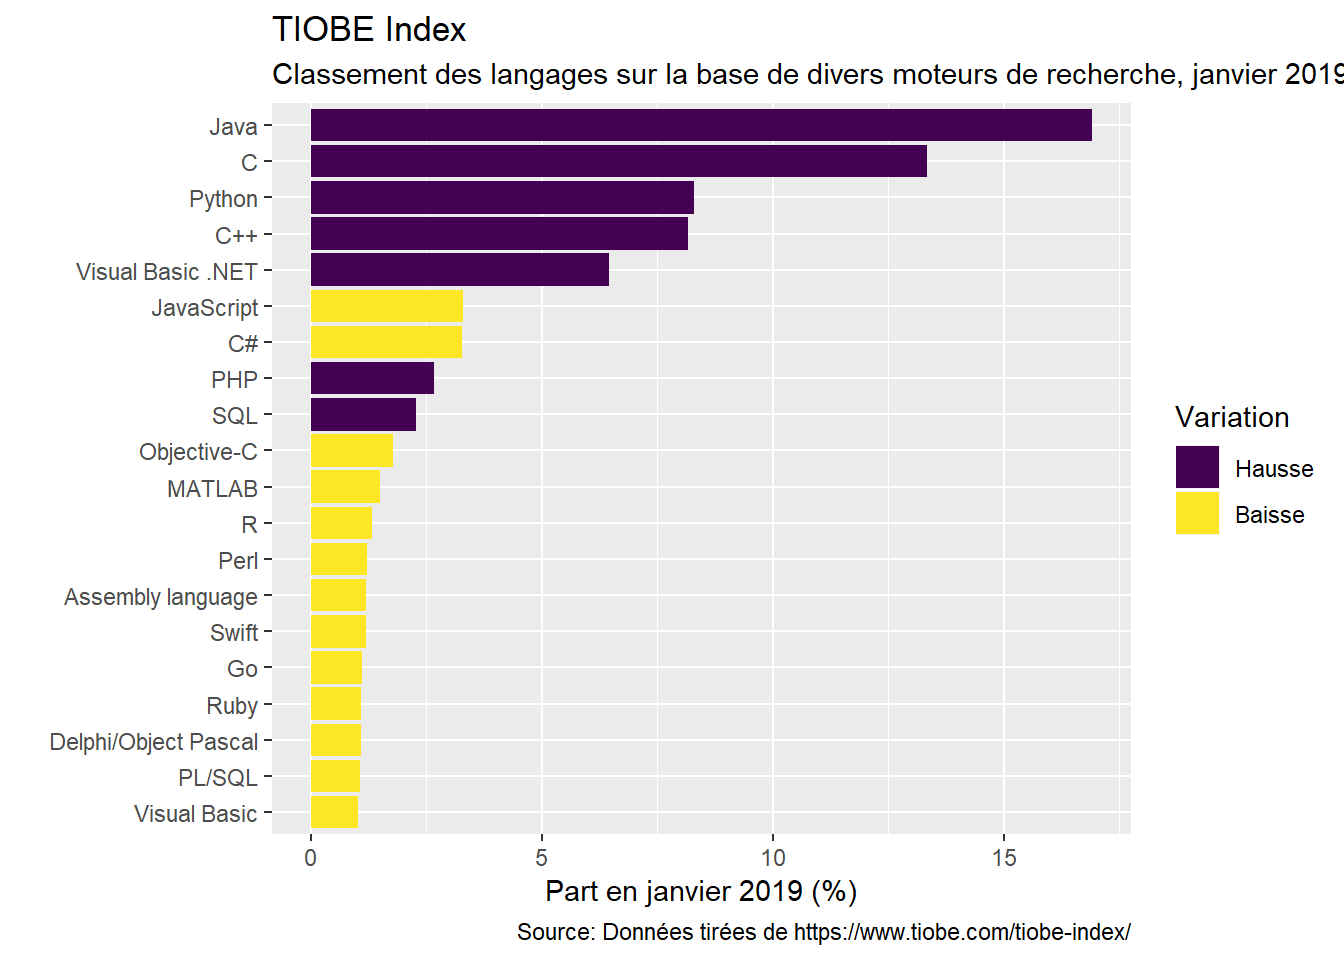
\includegraphics[width=1\linewidth,height=1\textheight]{dswr_book_files/figure-latex/unnamed-chunk-4-1}

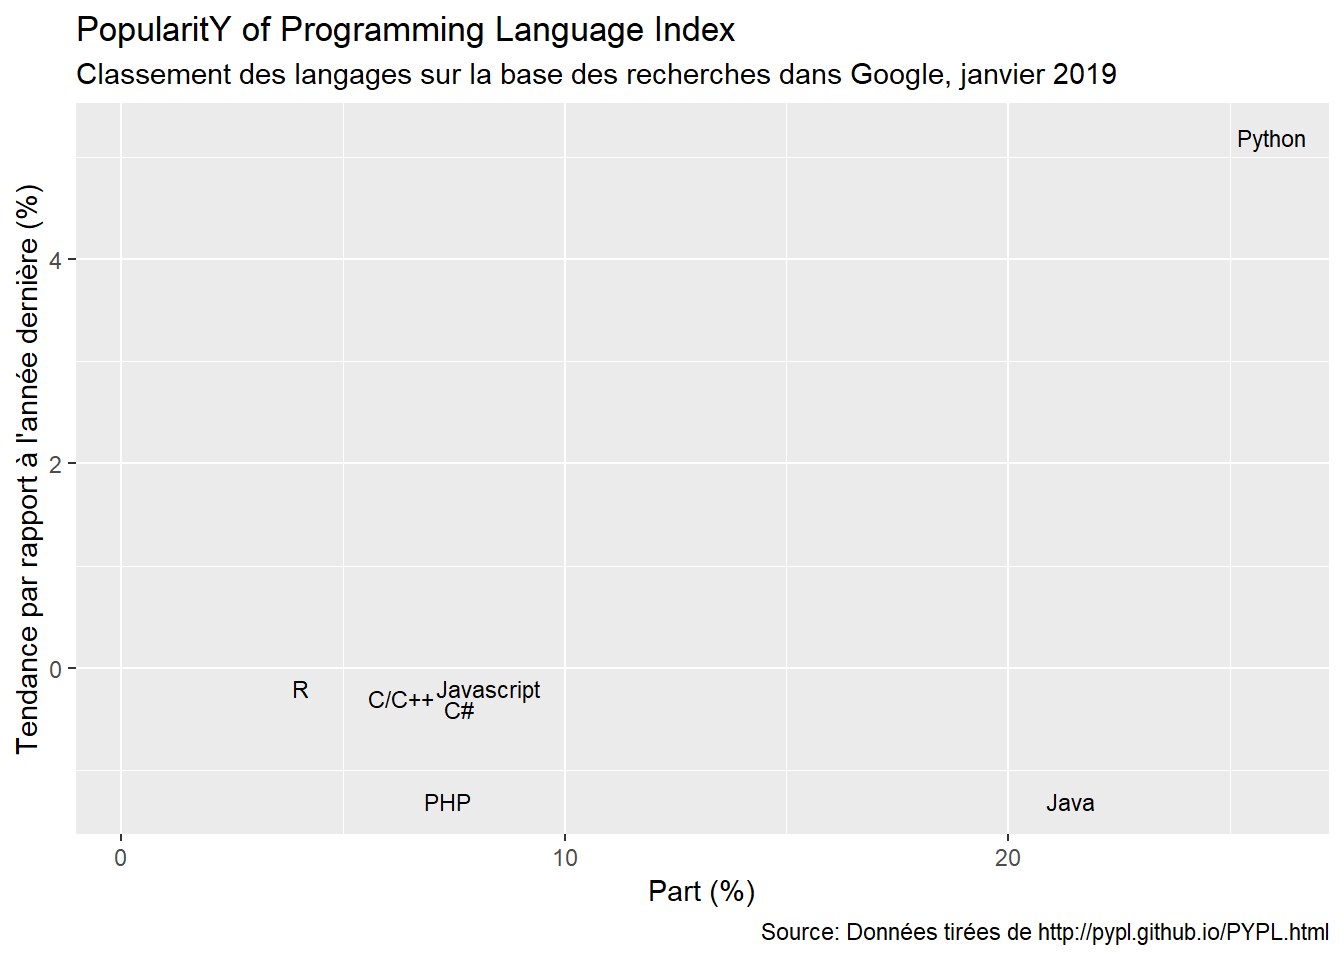
\includegraphics[width=1\linewidth,height=1\textheight]{dswr_book_files/figure-latex/unnamed-chunk-5-1}

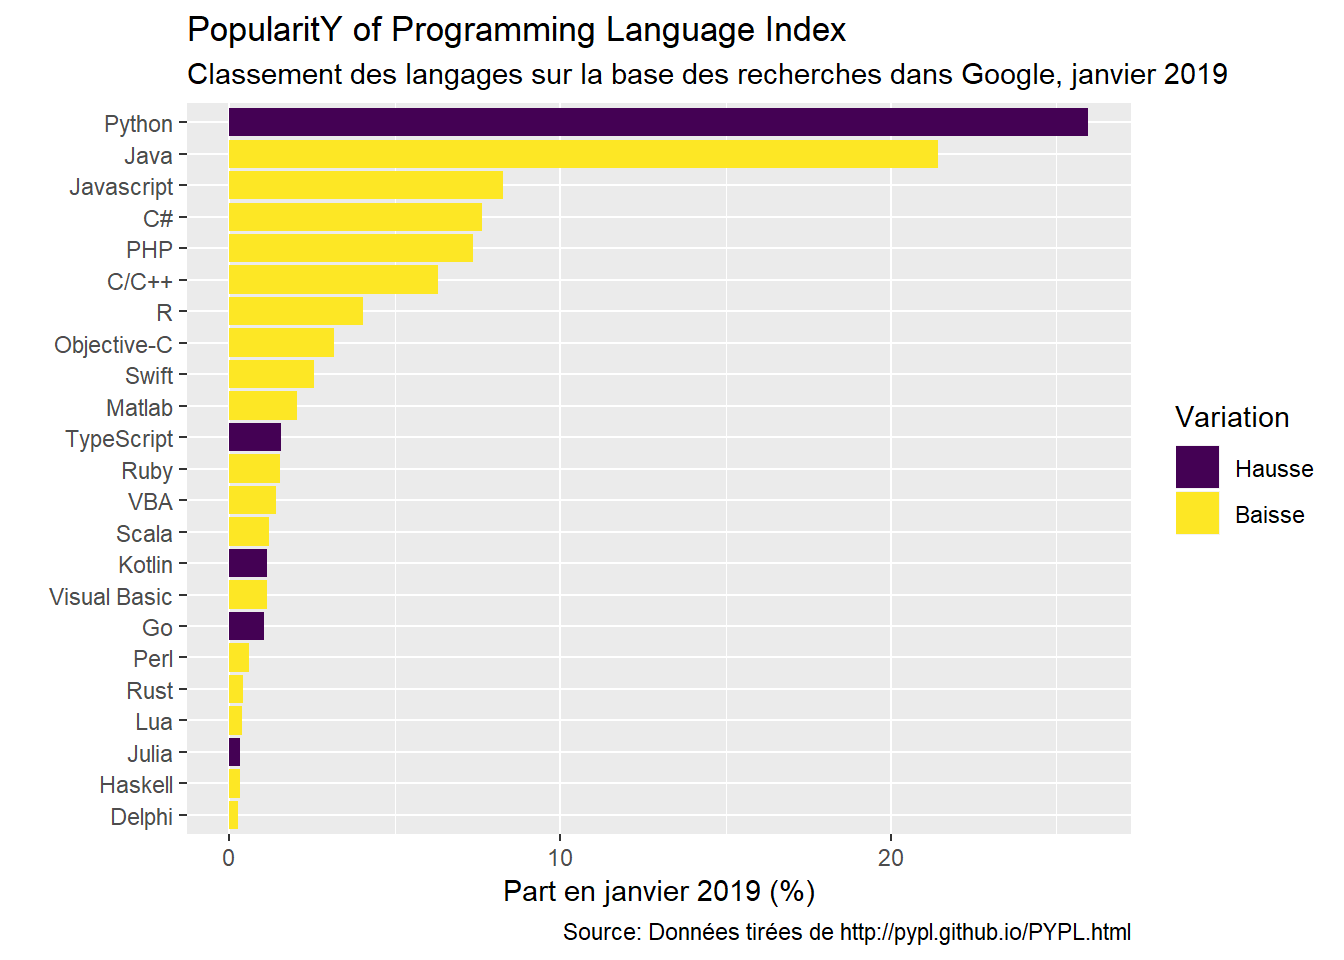
\includegraphics[width=1\linewidth,height=1\textheight]{dswr_book_files/figure-latex/unnamed-chunk-6-1}

Ce qui apparait des différentes figures, c'est que R parvient à se
tailler une place parmi les langages les plus populaires au monde. Et
celà, malgré le fait que c'est une langage spécialisée. Si sur les dix
dernières années, le langage s'est enrichi avec la diversification de
ses contributeurs, il reste à la base un langage élaboré par des
statisticiens pour des statisticiens. De ce fait, il est excéllent pour
l'analyse de données, mais fort peu utile pour certaines
tâches\ldots{}comme le développement d'un site web.

\section{RStudio}\label{rstudio}

\subsection{Qu'est-ce que c'est que
RStudio}\label{quest-ce-que-cest-que-rstudio}

\begin{itemize}
\item
  C'est une IDE (\emph{Integrated Development Environment}) ou
  Environnement Intégré de Développement
\item
  Il sert d'interface entre R et l'utilisateur, offre à celui diverses
  commodités d'utilisation
\end{itemize}

Maintenant, vous avez les outils nécéssaires pour commencer la
formidable aventuRe!

\chapter{Objets dans R}\label{objets-dans-r}

\section{Introduction}\label{introduction-1}

Dans ce chapitre, nous allons :

\begin{itemize}
\item
  introduire la notion d'objet dans R;
\item
  présenter un certain nombre d'entre eux;
\item
  et illustrer avec quelques exemples.
\end{itemize}

Que nous faudra-t-il?

\begin{itemize}
\item
  R (évidemment)
\item
  RStudio (de préférence)
\end{itemize}

\section{La notion d'objet dans R}\label{la-notion-dobjet-dans-r}

\subsection{Qu'est-ce qu'un objet?}\label{quest-ce-quun-objet}

Dans R, un objet représente un concept, une idée. Il se matérialise par
une entité qui possède sa propre identité. Dans celle-ci, l'on compte
deux aspects majeurs:

\begin{itemize}
\item
  la structure interne;
\item
  le comportement.
\end{itemize}

Illustrons pour comprendre. Commençons par créer des objets.

Imaginez que vous voulez créer et conserver des bouts d'information dans
R sur les présidents qui se sont succédés à la tête de la République du
Mali. Commençons par le premier président,
\href{https://fr.wikipedia.org/wiki/Modibo_Ke\%C3\%AFta_(1915-1977)}{Mobido
Keïta}. Créeons des objects relatifs à son nom et son prénom.

\begin{Shaded}
\begin{Highlighting}[]
\NormalTok{nom <-}\StringTok{ "Keïta"}
\NormalTok{prenom <-}\StringTok{ "Mobido"}
\end{Highlighting}
\end{Shaded}

L'acte d'assignation d'une valeur à un objet se fait par le signe
\texttt{\textless{}-} qui est équivalent à \texttt{=}. Chez beaucoup
d'utilisateurs, la préférence est donnée à la première. Ceci peut se
comprendre par le fait qu'avec \texttt{\textless{}-}, l'acte
d'assignation se différencie plus facilement d'autres utilisations du
signe \texttt{=} (dont notamment à l'intérieur de fonctions). Désormais,
ces informations sont stockées dans notre environnement. Pour vérifier
appellons-les! Ceci revient à les saisir dans notre console et à taper
``Entrée''!

\begin{Shaded}
\begin{Highlighting}[]
\NormalTok{nom}
\end{Highlighting}
\end{Shaded}

\begin{verbatim}
## [1] "Keïta"
\end{verbatim}

\begin{Shaded}
\begin{Highlighting}[]
\NormalTok{prenom}
\end{Highlighting}
\end{Shaded}

\begin{verbatim}
## [1] "Mobido"
\end{verbatim}

\subsection{Oranges et bananes}\label{oranges-et-bananes}

Enrichissons notre environnement des objets additionnels. Ajoutons
l'année d'accession au pouvoir. Appelons cet objet
\texttt{annee\_arrivee\_pouvoir}.

\begin{Shaded}
\begin{Highlighting}[]
\NormalTok{annee_arrivee_pouvoir <-}\StringTok{ }\DecValTok{1960}
\end{Highlighting}
\end{Shaded}

Comme pour les objets précédent, celui-ci aussi peut être invoqué:

\begin{Shaded}
\begin{Highlighting}[]
\NormalTok{annee_arrivee_pouvoir}
\end{Highlighting}
\end{Shaded}

\begin{verbatim}
## [1] 1960
\end{verbatim}

A l'instar de l'orange et de la banane, fort différentes bien que toutes
les deux des fruits, ici aussi nos objets diffèrent. Peut-on les
additionner?

\begin{Shaded}
\begin{Highlighting}[]
\NormalTok{nom }\OperatorTok{+}\StringTok{ }\NormalTok{annee_arrivee_pouvoir}
\end{Highlighting}
\end{Shaded}

\begin{verbatim}
## Error in nom + annee_arrivee_pouvoir: non-numeric argument to binary operator
\end{verbatim}

Non, en l'occurence! On a un message d'erreur. R, c'est comme la vraie
vie! Les oranges et les bananes ne se mélangent.

\subsection{Ce qui se ressemblent
s'assemblent}\label{ce-qui-se-ressemblent-sassemblent}

Les choses qui diffèrent ne s'assemblent pas Illustration d'une
propriété des objets: le comportement. Regardons les choses qui
marchent.

\begin{verbatim}
## [1] 2
\end{verbatim}

Maintenant stockons ce résultat dans un objet.

\begin{Shaded}
\begin{Highlighting}[]
\NormalTok{objet1 <-}\StringTok{ }\DecValTok{1} \OperatorTok{+}\StringTok{ }\DecValTok{1}
\end{Highlighting}
\end{Shaded}

Créons-en un autre.

\begin{Shaded}
\begin{Highlighting}[]
\NormalTok{objet2 <-}\StringTok{ }\DecValTok{2} \OperatorTok{+}\StringTok{ }\DecValTok{2}
\end{Highlighting}
\end{Shaded}

Amusons à faire diverses opérations avec ces deux objets

\begin{Shaded}
\begin{Highlighting}[]
\NormalTok{objet1 }\OperatorTok{+}\StringTok{ }\NormalTok{objet2}
\end{Highlighting}
\end{Shaded}

\begin{verbatim}
## [1] 6
\end{verbatim}

\begin{Shaded}
\begin{Highlighting}[]
\NormalTok{objet1 }\OperatorTok{-}\StringTok{ }\NormalTok{objet2}
\end{Highlighting}
\end{Shaded}

\begin{verbatim}
## [1] -2
\end{verbatim}

\begin{Shaded}
\begin{Highlighting}[]
\NormalTok{objet1 }\OperatorTok{*}\StringTok{ }\NormalTok{objet2}
\end{Highlighting}
\end{Shaded}

\begin{verbatim}
## [1] 8
\end{verbatim}

\begin{Shaded}
\begin{Highlighting}[]
\NormalTok{objet1 }\OperatorTok{/}\StringTok{ }\NormalTok{objet2}
\end{Highlighting}
\end{Shaded}

\begin{verbatim}
## [1] 0.5
\end{verbatim}

Bref, vous voyez l'idée! Les propriétés des objets déterminent les
intéractions auxquelles elles se prêtent. Et ce sont justement ces
intéractions qui constituent le coeur de l'analyse de données. D'où
l'importance de la notion d'objet.

\subsection{Quelques objets dans R}\label{quelques-objets-dans-r}

Dans R, l'on distingue plusieurs types d'objets. Nous en retiendrons ici
5, qui nous serons utiles tout le long de l'ouvrage. Il s'agit des:

\begin{itemize}
\item
  caractères (\emph{strings} en anglais);
\item
  nombres (entiers ou réels);
\item
  dates;
\item
  valeurs logiques qui ne prennent que deux valeurs: \texttt{TRUE}
  (vrai) ou \texttt{FALSE} (faux);
\item
  facteurs qui sont un format spécial dans R prévu pour les variables
  catégorielles.
\end{itemize}

Revenons à notre exemple \emph{présidentiel}! Nous avons déjà le nom et
le prénom\ldots{}

\begin{Shaded}
\begin{Highlighting}[]
\CommentTok{# Caractères}
\NormalTok{nom <-}\StringTok{ "Keïta"}
\NormalTok{prenom <-}\StringTok{ "Mobido"}
\end{Highlighting}
\end{Shaded}

\ldots{}ainsi que l'année d'arrivée au pouvoir.

\begin{Shaded}
\begin{Highlighting}[]
\CommentTok{# Nombre}
\NormalTok{annee_arrivee_pouvoir <-}\StringTok{ }\DecValTok{1960}
\end{Highlighting}
\end{Shaded}

Ajoutons la date de naissance,

\begin{Shaded}
\begin{Highlighting}[]
\CommentTok{# Date}
\NormalTok{date_naissance <-}\StringTok{ }\KeywordTok{as.Date}\NormalTok{(}\StringTok{"1915-06-04"}\NormalTok{)}
\end{Highlighting}
\end{Shaded}

une valeur logique indiquant s'il a eu un parcours militaire ou pas,

\begin{Shaded}
\begin{Highlighting}[]
\CommentTok{# Valeur logique}
\NormalTok{parcours_militaire <-}\StringTok{ }\OtherTok{FALSE}
\end{Highlighting}
\end{Shaded}

et enfin la région de naissance.

\begin{Shaded}
\begin{Highlighting}[]
\CommentTok{# Facteur}
\NormalTok{region_naissance <-}\StringTok{ }\KeywordTok{as.factor}\NormalTok{(}\StringTok{"Bamako"}\NormalTok{)}
\end{Highlighting}
\end{Shaded}

\subsection{La notion de classe et de
type}\label{la-notion-de-classe-et-de-type}

Quand on a faire à des objets dont on ignore l'identité, l'on peut
s'appuyer la fonction \texttt{class}. Celle-ci permet de connaître la
classe de l'objet. La classe est un attribut qui contribue à la
formation de l'idée d'un objet. ``Avec quoi se mélange-t-il?'' ``A
quelles règles de transformation se soumet-il?'' Basiquement, la classe
dicte les principes régissant la manipulation de cet objet. Testons la
fonction sur les objets que nous venons de créer pour bien confirmer les
identités qu'on leur a attribuées.

\begin{Shaded}
\begin{Highlighting}[]
\KeywordTok{class}\NormalTok{(nom)}
\end{Highlighting}
\end{Shaded}

\begin{verbatim}
## [1] "character"
\end{verbatim}

\begin{Shaded}
\begin{Highlighting}[]
\KeywordTok{class}\NormalTok{(prenom)}
\end{Highlighting}
\end{Shaded}

\begin{verbatim}
## [1] "character"
\end{verbatim}

\begin{Shaded}
\begin{Highlighting}[]
\KeywordTok{class}\NormalTok{(annee_arrivee_pouvoir)}
\end{Highlighting}
\end{Shaded}

\begin{verbatim}
## [1] "numeric"
\end{verbatim}

\begin{Shaded}
\begin{Highlighting}[]
\KeywordTok{class}\NormalTok{(date_naissance)}
\end{Highlighting}
\end{Shaded}

\begin{verbatim}
## [1] "Date"
\end{verbatim}

\begin{Shaded}
\begin{Highlighting}[]
\KeywordTok{class}\NormalTok{(parcours_militaire)}
\end{Highlighting}
\end{Shaded}

\begin{verbatim}
## [1] "logical"
\end{verbatim}

\begin{Shaded}
\begin{Highlighting}[]
\KeywordTok{class}\NormalTok{(region_naissance)}
\end{Highlighting}
\end{Shaded}

\begin{verbatim}
## [1] "factor"
\end{verbatim}

Nous voyons que les résultats sont bien conformes aux dénominations que
nous leur avons données plus haut.

Dans R, il y a aussi la fonction \texttt{typeof} (ou \texttt{mode}, mais
nous resterons avec la première) qui permet de connaître le mode de
stockage d'un objet. Testons!

\begin{Shaded}
\begin{Highlighting}[]
\KeywordTok{typeof}\NormalTok{(nom)}
\end{Highlighting}
\end{Shaded}

\begin{verbatim}
## [1] "character"
\end{verbatim}

\begin{Shaded}
\begin{Highlighting}[]
\KeywordTok{typeof}\NormalTok{(prenom)}
\end{Highlighting}
\end{Shaded}

\begin{verbatim}
## [1] "character"
\end{verbatim}

\begin{Shaded}
\begin{Highlighting}[]
\KeywordTok{typeof}\NormalTok{(annee_arrivee_pouvoir)}
\end{Highlighting}
\end{Shaded}

\begin{verbatim}
## [1] "double"
\end{verbatim}

\begin{Shaded}
\begin{Highlighting}[]
\KeywordTok{typeof}\NormalTok{(date_naissance)}
\end{Highlighting}
\end{Shaded}

\begin{verbatim}
## [1] "double"
\end{verbatim}

\begin{Shaded}
\begin{Highlighting}[]
\KeywordTok{typeof}\NormalTok{(parcours_militaire)}
\end{Highlighting}
\end{Shaded}

\begin{verbatim}
## [1] "logical"
\end{verbatim}

\begin{Shaded}
\begin{Highlighting}[]
\KeywordTok{typeof}\NormalTok{(region_naissance)}
\end{Highlighting}
\end{Shaded}

\begin{verbatim}
## [1] "integer"
\end{verbatim}

Si pour les objets \texttt{nom} et \texttt{prenom} qui sont des lettres,
la classe et le type se confondent, la question est tout autre pour
d'autres objets. Regardons \texttt{region\_naissance}, par exemple. En
termes de classe, c'est un facteur. Par contre, en terme de type, R l'a
coercé en entier (\emph{integer}).

Les types sont assez génériques car présentant pratiquement les mêmes
nomenclatures d'un langage à un autre. Dans R, nous allons plus nous
intéressér aux types suivants:

\begin{itemize}
\item
  logique (\emph{logical});
\item
  entier (\emph{integer});
\item
  réel (\emph{double});
\item
  caractère (\emph{character});
\item
  liste (\emph{list});
\item
  valeur nulle (\emph{NULL}).
\end{itemize}

Les objets que nous avons vus là peuvent être pensés comme des briques.
Ils entrent à leur tour dans la formation d'autres objets qui varient
les uns des autres. Tout comme les constructions peuvent différer entre
elles.

\subsection{Vers d'autres types
d'objets}\label{vers-dautres-types-dobjets}

Les objets que nous allons voir ici peuvent être pensés comme des objets
composites. Nous en verrons quatre types:

\begin{itemize}
\item
  le vecteur;
\item
  la matrice;
\item
  le \emph{data frame} (cadre de données ou données rectangulaires);
\item
  la liste.
\end{itemize}

\section{Vecteurs}\label{vecteurs}

\subsection{Qu'est-ce qu'un vecteur?}\label{quest-ce-quun-vecteur}

De façon très simple, un vecteur est un ensemble d'éléments de même
nature. Revenons à notre exemple pour mieux comprendre. Nous avons
défini l'objet \texttt{nom}, n'est-ce pas? Est-ce un vecteur? A quoi
peut-on voir si c'est un vecteur ou pas? La réponse:

\begin{Shaded}
\begin{Highlighting}[]
\KeywordTok{is.vector}\NormalTok{(nom)}
\end{Highlighting}
\end{Shaded}

\begin{verbatim}
## [1] TRUE
\end{verbatim}

Donc nous avons crééé des vecteurs depuis longtemps et on voit qu'un
objet d'un seul élément peut être un vecteur. Maintenant, comptons le
nombre d'éléments que compte ce vecteur.

\begin{Shaded}
\begin{Highlighting}[]
\KeywordTok{length}\NormalTok{(nom)}
\end{Highlighting}
\end{Shaded}

\begin{verbatim}
## [1] 1
\end{verbatim}

C'est vraiment un singleton qu'on a là\ldots{}pour le moment!

\subsection{Créons-en, des vecteurs!}\label{creons-en-des-vecteurs}

Décidons d'étendre nos observations à tous les présidents de la
République du Mali. En voici de quoi nous faire revisiter nos livres
d'histoire\ldots{}ou juste consulter Wikipedia!

\begin{Shaded}
\begin{Highlighting}[]
\CommentTok{# Omettons les périodes de transition (la valeur pédagogique est ce qui est recherché ici!)}
\NormalTok{nom <-}\StringTok{ }\KeywordTok{c}\NormalTok{(}\StringTok{"Keïta"}\NormalTok{, }\StringTok{"Traoré"}\NormalTok{, }\StringTok{"Konaré"}\NormalTok{, }\StringTok{"Touré"}\NormalTok{, }\StringTok{"Keïta"}\NormalTok{)}
\NormalTok{prenom <-}\StringTok{ }\KeywordTok{c}\NormalTok{(}\StringTok{"Modibo"}\NormalTok{, }\StringTok{"Moussa"}\NormalTok{, }\StringTok{"Alpha Oumar"}\NormalTok{, }\StringTok{"Amadou Toumani"}\NormalTok{, }\StringTok{"Ibrahim Boubacar"}\NormalTok{)}
\NormalTok{date_naissance <-}\StringTok{ }\KeywordTok{as.Date}\NormalTok{(}\KeywordTok{c}\NormalTok{(}\StringTok{"1915-06-04"}\NormalTok{, }\StringTok{"1936-09-25"}\NormalTok{, }\StringTok{"1946-02-02"}\NormalTok{, }\StringTok{"1948-11-04"}\NormalTok{, }\StringTok{"1945-01-29"}\NormalTok{))}
\NormalTok{region_naissance <-}\StringTok{ }\KeywordTok{as.factor}\NormalTok{(}\KeywordTok{c}\NormalTok{(}\StringTok{"Bamako"}\NormalTok{, }\StringTok{"Kayes"}\NormalTok{, }\StringTok{"Kayes"}\NormalTok{, }\StringTok{"Mopti"}\NormalTok{, }\StringTok{"Koutiala"}\NormalTok{))}
\NormalTok{annee_arrivee_pouvoir <-}\StringTok{ }\KeywordTok{c}\NormalTok{(}\DecValTok{1960}\NormalTok{, }\DecValTok{1968}\NormalTok{, }\DecValTok{1992}\NormalTok{, }\DecValTok{2002}\NormalTok{, }\DecValTok{2013}\NormalTok{)}
\NormalTok{parcours_militaire <-}\StringTok{ }\KeywordTok{c}\NormalTok{(}\OtherTok{FALSE}\NormalTok{, }\OtherTok{TRUE}\NormalTok{, }\OtherTok{FALSE}\NormalTok{, }\OtherTok{TRUE}\NormalTok{, }\OtherTok{FALSE}\NormalTok{)}
\end{Highlighting}
\end{Shaded}

Maintenant, expérimentons! Commençons avec \texttt{nom} que nous avons
écrasé avec de nouvelles valeurs.

\begin{Shaded}
\begin{Highlighting}[]
\KeywordTok{is.vector}\NormalTok{(nom)}
\end{Highlighting}
\end{Shaded}

\begin{verbatim}
## [1] TRUE
\end{verbatim}

\begin{Shaded}
\begin{Highlighting}[]
\KeywordTok{length}\NormalTok{(nom)}
\end{Highlighting}
\end{Shaded}

\begin{verbatim}
## [1] 5
\end{verbatim}

\begin{Shaded}
\begin{Highlighting}[]
\KeywordTok{class}\NormalTok{(nom)}
\end{Highlighting}
\end{Shaded}

\begin{verbatim}
## [1] "character"
\end{verbatim}

\begin{Shaded}
\begin{Highlighting}[]
\KeywordTok{typeof}\NormalTok{(nom)}
\end{Highlighting}
\end{Shaded}

\begin{verbatim}
## [1] "character"
\end{verbatim}

``nom'' est un \textbf{vecteur}, un ensemble de \textbf{5} éléments en
\textbf{charactères}. Amusez-vous à expérimenter avec les autres
vecteurs.

\subsection{Vrai pour un, vrai pour
plusieurs}\label{vrai-pour-un-vrai-pour-plusieurs}

Vous vous rappelez que plus haut, nous voyions que les opérations
n'étaient pas possibles entre de différentes natures. Et bien, cette
règle, valable à l'échelle des objets élémentaires, l'est aussi aux
échelles supérieures.

Prenons nos données et cherchons à déterminer l'âge des présidents à
leur arrivée au pouvoir. On a les éléments nécéssaires pour ce faire, la
date de naissance et l'année d'arrivée au pouvoir. Toutefois, ces deux
vecteurs ne sont pas de même nature.

\begin{Shaded}
\begin{Highlighting}[]
\NormalTok{age_arrivee_pouvoir <-}\StringTok{ }\NormalTok{annee_arrivee_pouvoir }\OperatorTok{-}\StringTok{ }\NormalTok{date_naissance}
\end{Highlighting}
\end{Shaded}

\begin{verbatim}
## Error in `-.Date`(annee_arrivee_pouvoir, date_naissance): can only subtract from "Date" objects
\end{verbatim}

On a un message d'erreur. Apparemment l'opération n'est pas possible. Il
faudrait procéder à une transformation: déduire de la date de naissance
l'année pour conduire l'opération avec celle-ci.

\begin{Shaded}
\begin{Highlighting}[]
\NormalTok{annee_naissance <-}\StringTok{ }\KeywordTok{as.numeric}\NormalTok{(}\KeywordTok{format}\NormalTok{(date_naissance,}\StringTok{'%Y'}\NormalTok{))}
\end{Highlighting}
\end{Shaded}

Testons si le nouveau vecteur est de même nature de celui de
\texttt{annee\_arrivee\_pouvoir}.

\begin{Shaded}
\begin{Highlighting}[]
\KeywordTok{class}\NormalTok{(annee_naissance)}
\end{Highlighting}
\end{Shaded}

\begin{verbatim}
## [1] "numeric"
\end{verbatim}

Maintenant, nous pouvons procéder à l'opération

\begin{Shaded}
\begin{Highlighting}[]
\NormalTok{age_arrivee_pouvoir <-}\StringTok{ }\NormalTok{annee_arrivee_pouvoir }\OperatorTok{-}\StringTok{ }\NormalTok{annee_naissance}
\NormalTok{age_arrivee_pouvoir}
\end{Highlighting}
\end{Shaded}

\begin{verbatim}
## [1] 45 32 46 54 68
\end{verbatim}

On le confirme: les oranges et les bananes ne se mélangent pas.
Toutefois, R nous fait souvent des cocktails de fruits en coerçant
certains éléments. Imaginons que l'on veuille rassembler le prénom et le
nom dans un seul vecteur. Collons ces éléments à l'aide d'une fonction
de base dans R, \texttt{paste}, (ne vous en faites pas, vous ferez
progressivement connaissance avec les fonctions!)

\begin{Shaded}
\begin{Highlighting}[]
\NormalTok{prenom_nom <-}\StringTok{ }\KeywordTok{paste}\NormalTok{(prenom, nom)}
\NormalTok{prenom_nom}
\end{Highlighting}
\end{Shaded}

\begin{verbatim}
## [1] "Modibo Keïta"           "Moussa Traoré"         
## [3] "Alpha Oumar Konaré"     "Amadou Toumani Touré"  
## [5] "Ibrahim Boubacar Keïta"
\end{verbatim}

On peut être enclin à dire que ceci est passé sans souci parce que
\texttt{nom} et \texttt{prenom} sont tous les deux des vecteurs en
caractères. Maintenant, et si l'on ajoutait l'année d'arrivée au
pouvoir?

\begin{Shaded}
\begin{Highlighting}[]
\NormalTok{prenom_nom_age <-}\StringTok{ }\KeywordTok{paste}\NormalTok{(prenom, nom, }\StringTok{","}\NormalTok{, age_arrivee_pouvoir)}
\NormalTok{prenom_nom_age}
\end{Highlighting}
\end{Shaded}

\begin{verbatim}
## [1] "Modibo Keïta , 45"           "Moussa Traoré , 32"         
## [3] "Alpha Oumar Konaré , 46"     "Amadou Toumani Touré , 54"  
## [5] "Ibrahim Boubacar Keïta , 68"
\end{verbatim}

C'est passé comme une lettre à la poste (pour la génération email, voici
ce qu'est \href{https://fr.wikipedia.org/wiki/Poste}{la poste}). Car R a
une hiérarchie entre les objets. Avant de déclarer forfait avec un
message d'erreur, il tente tant bien que mal d'exécuter l'opération. Sur
la base de cette hiérarchie, il coerce certains éléments à se conformer
à d'autres, partant du plus flexible au moins flexible: \texttt{logique}
\textless{} \texttt{entier} \textless{} \texttt{réel} \textless{}
\texttt{caractère}. Pour comprendre ça, créons un vecteur de valeurs
logiques.

\begin{Shaded}
\begin{Highlighting}[]
\NormalTok{vecteur_logique <-}\StringTok{ }\KeywordTok{c}\NormalTok{(}\OtherTok{TRUE}\NormalTok{, }\OtherTok{FALSE}\NormalTok{)}
\end{Highlighting}
\end{Shaded}

Confirmons sa classe.

\begin{Shaded}
\begin{Highlighting}[]
\KeywordTok{class}\NormalTok{(vecteur_logique)}
\end{Highlighting}
\end{Shaded}

\begin{verbatim}
## [1] "logical"
\end{verbatim}

Ajoutons un troisième élément qui sera un entier. Disons 1.

\begin{Shaded}
\begin{Highlighting}[]
\NormalTok{vecteur_entier <-}\StringTok{ }\KeywordTok{c}\NormalTok{(vecteur_logique, }\DecValTok{1}\NormalTok{)}
\end{Highlighting}
\end{Shaded}

Qu'obtenons-nous?

\begin{Shaded}
\begin{Highlighting}[]
\NormalTok{vecteur_entier}
\end{Highlighting}
\end{Shaded}

\begin{verbatim}
## [1] 1 0 1
\end{verbatim}

Des entiers! R a coercé \texttt{TRUE} en 1 et \texttt{FALSE} en 0.

\begin{Shaded}
\begin{Highlighting}[]
\KeywordTok{class}\NormalTok{(vecteur_entier)}
\end{Highlighting}
\end{Shaded}

\begin{verbatim}
## [1] "numeric"
\end{verbatim}

Ajoutons un quatrième élément, cette fois-ci une réel: 2.5 (dans R,
comme en anglais, les décimales viennent après un \texttt{.}, pas une
\texttt{,}, qui sert plutôt de séparateur de milliers).

\begin{Shaded}
\begin{Highlighting}[]
\NormalTok{vecteur_reel <-}\StringTok{ }\KeywordTok{c}\NormalTok{(vecteur_entier, }\FloatTok{2.5}\NormalTok{)}
\NormalTok{vecteur_reel}
\end{Highlighting}
\end{Shaded}

\begin{verbatim}
## [1] 1.0 0.0 1.0 2.5
\end{verbatim}

\begin{Shaded}
\begin{Highlighting}[]
\KeywordTok{class}\NormalTok{(vecteur_reel)}
\end{Highlighting}
\end{Shaded}

\begin{verbatim}
## [1] "numeric"
\end{verbatim}

La mutation se voit au fait que R a affecté aux trois premiers éléments
des décimales, bien qu'initialement c'étaient des entiers. Maintenant,
ajoutons un cinquième élément: un prénom.

\begin{Shaded}
\begin{Highlighting}[]
\NormalTok{vecteur_caractere <-}\StringTok{ }\KeywordTok{c}\NormalTok{(vecteur_reel, }\StringTok{"Mariam"}\NormalTok{)}
\NormalTok{vecteur_caractere}
\end{Highlighting}
\end{Shaded}

\begin{verbatim}
## [1] "1"      "0"      "1"      "2.5"    "Mariam"
\end{verbatim}

\begin{Shaded}
\begin{Highlighting}[]
\KeywordTok{class}\NormalTok{(vecteur_caractere)}
\end{Highlighting}
\end{Shaded}

\begin{verbatim}
## [1] "character"
\end{verbatim}

Là aussi, la coercion se voit.

\subsection{Nommer les éléments d'un
vecteur}\label{nommer-les-elements-dun-vecteur}

Jusque là, ce sont des objets à part intégrale que nous avons nommés. On
les a assignés des noms pour les garder dans notre environnement de
travail. Maintenant, nous allons donner un nom aux éléments de vecteur.
Dressons l'analogie suivante. Notre environnement dans R est comme une
rue. Dans celle-ci, nous avons des concessions dont les portes sont
toutes numérotées: ce sont les noms des objets. A l'intérieur des
concessions, nous avons des individus: ce sont les éléments à
l'intérieur de nos objets. Tout comme ces individus portent des prénoms,
nous pouvons donner des appélations aux éléments contenus dans nos
objets.

Considerons que nous voulons associer à chaque date de naissance le nom
du président en question.

\begin{Shaded}
\begin{Highlighting}[]
\KeywordTok{names}\NormalTok{(date_naissance) <-}\StringTok{ }\NormalTok{prenom_nom}
\end{Highlighting}
\end{Shaded}

Voyons ce que ça donne

\begin{Shaded}
\begin{Highlighting}[]
\NormalTok{date_naissance}
\end{Highlighting}
\end{Shaded}

\begin{verbatim}
##           Modibo Keïta          Moussa Traoré     Alpha Oumar Konaré 
##           "1915-06-04"           "1936-09-25"           "1946-02-02" 
##   Amadou Toumani Touré Ibrahim Boubacar Keïta 
##           "1948-11-04"           "1945-01-29"
\end{verbatim}

C'est beau non! Il est intéréssant de noter que quand on conduit des
opérations sur des vecteurs aux éléments nommés, le résultat peut
hériter de ces propriétés. Reprenons l'opération de déduction de l'âge à
l'arrivée au pouvoir. Rappelons les deux vecteurs.

\begin{Shaded}
\begin{Highlighting}[]
\NormalTok{annee_naissance}
\end{Highlighting}
\end{Shaded}

\begin{verbatim}
## [1] 1915 1936 1946 1948 1945
\end{verbatim}

\begin{Shaded}
\begin{Highlighting}[]
\NormalTok{annee_arrivee_pouvoir}
\end{Highlighting}
\end{Shaded}

\begin{verbatim}
## [1] 1960 1968 1992 2002 2013
\end{verbatim}

Nommons juste un des deux vecteurs.

\begin{Shaded}
\begin{Highlighting}[]
\KeywordTok{names}\NormalTok{(annee_naissance) <-}\StringTok{ }\NormalTok{prenom_nom}
\NormalTok{annee_naissance}
\end{Highlighting}
\end{Shaded}

\begin{verbatim}
##           Modibo Keïta          Moussa Traoré     Alpha Oumar Konaré 
##                   1915                   1936                   1946 
##   Amadou Toumani Touré Ibrahim Boubacar Keïta 
##                   1948                   1945
\end{verbatim}

Procédons à l'opération.

\begin{Shaded}
\begin{Highlighting}[]
\NormalTok{age_arrivee_pouvoir <-}\StringTok{ }\NormalTok{annee_arrivee_pouvoir }\OperatorTok{-}\StringTok{ }\NormalTok{annee_naissance}
\NormalTok{age_arrivee_pouvoir}
\end{Highlighting}
\end{Shaded}

\begin{verbatim}
##           Modibo Keïta          Moussa Traoré     Alpha Oumar Konaré 
##                     45                     32                     46 
##   Amadou Toumani Touré Ibrahim Boubacar Keïta 
##                     54                     68
\end{verbatim}

Le vecteur \texttt{age\_arrivee\_pouvoir} a hérité des noms d'éléments.

Cette règle n'est pas toutefois immuable. Quand les éléments sont
coercés à prendre une autre classe que leur classe de départ, ils
peuvent perdre leur nom, qui n'est qu'un de leurs attributs (qui sont
subordonnés à leur classe). Reprenons la déduction de l'année de
naissance à partir de la date de naissance.

\begin{Shaded}
\begin{Highlighting}[]
\NormalTok{annee_naissance <-}\StringTok{ }\KeywordTok{format}\NormalTok{(date_naissance,}\StringTok{'%Y'}\NormalTok{)}
\NormalTok{annee_naissance}
\end{Highlighting}
\end{Shaded}

\begin{verbatim}
##           Modibo Keïta          Moussa Traoré     Alpha Oumar Konaré 
##                 "1915"                 "1936"                 "1946" 
##   Amadou Toumani Touré Ibrahim Boubacar Keïta 
##                 "1948"                 "1945"
\end{verbatim}

\begin{Shaded}
\begin{Highlighting}[]
\KeywordTok{class}\NormalTok{(annee_naissance)}
\end{Highlighting}
\end{Shaded}

\begin{verbatim}
## [1] "character"
\end{verbatim}

Ici, l'année n'a pas été coercé. Elle a été extraite par la fonction
sous format de caractères. En voulant conformer le vecteur à la classe
de nombre (on descend dans la hiérarchie), on coerce les éléments.

\begin{Shaded}
\begin{Highlighting}[]
\NormalTok{annee_naissance <-}\StringTok{ }\KeywordTok{as.numeric}\NormalTok{(}\KeywordTok{format}\NormalTok{(date_naissance,}\StringTok{'%Y'}\NormalTok{))}
\NormalTok{annee_naissance}
\end{Highlighting}
\end{Shaded}

\begin{verbatim}
## [1] 1915 1936 1946 1948 1945
\end{verbatim}

\begin{Shaded}
\begin{Highlighting}[]
\KeywordTok{class}\NormalTok{(annee_naissance)}
\end{Highlighting}
\end{Shaded}

\begin{verbatim}
## [1] "numeric"
\end{verbatim}

Avec la coercion, les noms se perdent. Il est donc utile de se rappeler
que les noms d'éléments ne sont pas immunes à la coercion. Toutefois,
quand les opérations se passent entre des éléments de même nature, les
noms sont bien saufs!

\subsection{Opérations sur vecteurs}\label{operations-sur-vecteurs}

\subsubsection{Sélection explicite}\label{selection-explicite}

Il arrive souvent qu'on ne soit intéréssée que par un élément précis
d'un vecteur. Peut-être l'on souhaite connaître seulement l'âge du
premier président lors de son accès au pouvoir. C'est le premier élément
du vecteur \texttt{age\_arrivee\_pouvoir}.

\begin{Shaded}
\begin{Highlighting}[]
\NormalTok{age_arrivee_pouvoir[}\DecValTok{1}\NormalTok{]}
\end{Highlighting}
\end{Shaded}

\begin{verbatim}
## Modibo Keïta 
##           45
\end{verbatim}

Peut-être nous voulons l'information pour le 1er et le 3ème présidents.
Ce sont les 1er et 3ème éléments du vecteur.

\begin{Shaded}
\begin{Highlighting}[]
\NormalTok{age_arrivee_pouvoir[}\KeywordTok{c}\NormalTok{(}\DecValTok{1}\NormalTok{, }\DecValTok{3}\NormalTok{)]}
\end{Highlighting}
\end{Shaded}

\begin{verbatim}
##       Modibo Keïta Alpha Oumar Konaré 
##                 45                 46
\end{verbatim}

Peut-être que nous voulons l'information du 1er au 3ème président.

\begin{Shaded}
\begin{Highlighting}[]
\NormalTok{age_arrivee_pouvoir[}\KeywordTok{c}\NormalTok{(}\DecValTok{1}\OperatorTok{:}\DecValTok{3}\NormalTok{)]}
\end{Highlighting}
\end{Shaded}

\begin{verbatim}
##       Modibo Keïta      Moussa Traoré Alpha Oumar Konaré 
##                 45                 32                 46
\end{verbatim}

On peut aussi souhaiter exclure certains éléments. Imaginons que l'on
veuille seulement regarder les informations sans les deux derniers
éléments du vecteur.

\begin{Shaded}
\begin{Highlighting}[]
\NormalTok{age_arrivee_pouvoir[}\OperatorTok{-}\KeywordTok{c}\NormalTok{(}\DecValTok{4}\NormalTok{, }\DecValTok{5}\NormalTok{)]}
\end{Highlighting}
\end{Shaded}

\begin{verbatim}
##       Modibo Keïta      Moussa Traoré Alpha Oumar Konaré 
##                 45                 32                 46
\end{verbatim}

Le signe \texttt{{[}{]}} agit comme une porte d'entrée à l'intérieur du
vecteur tandis que les chiffres indiqués sont des index qui indiquent la
position des éléments intérêt. L'opération peut consister en une
sélection ou une exclusion selon que l'opérateur \texttt{c} est précédé
du signe \texttt{-} (exclusion) ou pas (sélection).

\subsubsection{Sélection à partir de
logiques}\label{selection-a-partir-de-logiques}

La sélection à l'intérieur d'un vecteur peut aussi se faire à partir de
valeurs logiques. L'on peut poser des critères auxquels certains
éléments répondraient. Et sur la base de leur confirmité au(x)
critère(s) posé(s), l'on pourra effectuer la sélection (ou l'exclusion).
Cette fonctionnalité est très utile car elle permet au data scientist
d'utiliser les questions qu'il se pose pour avoir un aperçu des données
qui sont à sa disposition.

Explorons la question suivante: quels sont les présidents arrivés au
pouvoir avant l'âge de 50 ans?

\begin{Shaded}
\begin{Highlighting}[]
\NormalTok{president_avant_50ans <-}\StringTok{ }\NormalTok{age_arrivee_pouvoir }\OperatorTok{<}\StringTok{ }\DecValTok{50}
\NormalTok{president_avant_50ans}
\end{Highlighting}
\end{Shaded}

\begin{verbatim}
##           Modibo Keïta          Moussa Traoré     Alpha Oumar Konaré 
##                   TRUE                   TRUE                   TRUE 
##   Amadou Toumani Touré Ibrahim Boubacar Keïta 
##                  FALSE                  FALSE
\end{verbatim}

On transforme maintenant ce vecteur de valeurs logiques en outil de
sélection. On peut soir regarder le nom de ces présidents:

\begin{Shaded}
\begin{Highlighting}[]
\NormalTok{prenom_nom[president_avant_50ans]}
\end{Highlighting}
\end{Shaded}

\begin{verbatim}
## [1] "Modibo Keïta"       "Moussa Traoré"      "Alpha Oumar Konaré"
\end{verbatim}

Le résultat nous donne le nom des présidents pour lesquels le vecteur de
valeurs logiques affiche \texttt{TRUE}. On peut utiliser le même critère
sur d'autres vecteurs. Voyons le vecteur d'âge d'arrivée au pouvoir:
quel âge avec les présidents qui sont arrivés au pouvoir avant l'âge de
50 ans?

\begin{Shaded}
\begin{Highlighting}[]
\NormalTok{age_arrivee_pouvoir[age_arrivee_pouvoir }\OperatorTok{<}\StringTok{ }\DecValTok{50}\NormalTok{]}
\end{Highlighting}
\end{Shaded}

\begin{verbatim}
##       Modibo Keïta      Moussa Traoré Alpha Oumar Konaré 
##                 45                 32                 46
\end{verbatim}

Pendant qu'on y est, dans quelle région sont-ils nés?

\begin{Shaded}
\begin{Highlighting}[]
\KeywordTok{names}\NormalTok{(region_naissance) <-}\StringTok{ }\NormalTok{prenom_nom }\CommentTok{# nommons d'abord les éléments}
\NormalTok{region_naissance[age_arrivee_pouvoir }\OperatorTok{<}\StringTok{ }\DecValTok{50}\NormalTok{]}
\end{Highlighting}
\end{Shaded}

\begin{verbatim}
##       Modibo Keïta      Moussa Traoré Alpha Oumar Konaré 
##             Bamako              Kayes              Kayes 
## Levels: Bamako Kayes Koutiala Mopti
\end{verbatim}

Vous comprenez la logique\ldots{}

\subsubsection{Statistiques sommaires}\label{statistiques-sommaires}

Une fois le vecteur constitué, il peut en lui-même faire l'objet
d'opérations diverses. Posons diverses questions avec le vecteur
\texttt{age\_arrivee\_pouvoir}. Quelle est la moyenne d'âge d'arrivée au
pouvoir sur la base des éléments disponibles?

\begin{Shaded}
\begin{Highlighting}[]
\KeywordTok{mean}\NormalTok{(age_arrivee_pouvoir)}
\end{Highlighting}
\end{Shaded}

\begin{verbatim}
## [1] 49
\end{verbatim}

\begin{Shaded}
\begin{Highlighting}[]
\CommentTok{# une alternative donnat le même résultat.}
\KeywordTok{sum}\NormalTok{(age_arrivee_pouvoir)}\OperatorTok{/}\KeywordTok{length}\NormalTok{(age_arrivee_pouvoir)}
\end{Highlighting}
\end{Shaded}

\begin{verbatim}
## [1] 49
\end{verbatim}

Quel est l'âge d'arrivée au pouvoir le plus bas ?

\begin{Shaded}
\begin{Highlighting}[]
\KeywordTok{min}\NormalTok{(age_arrivee_pouvoir)}
\end{Highlighting}
\end{Shaded}

\begin{verbatim}
## [1] 32
\end{verbatim}

Quel est l'âge d'arrivée au pouvoir le plus élevé ?

\begin{verbatim}
## [1] 68
\end{verbatim}

\subsubsection{Ajustement et recyclage}\label{ajustement-et-recyclage}

Maintenant, revenons-en un peu aux opérations entre deux vecteurs.
Imaginez maintenant, que l'on veuille connaître l'âge auquel les
présidents ont quitté le pouvoir. Rappellons d'abord le vecteur
\texttt{age\_arrivee\_pouvoir} que nous avions déjà généré.

\begin{Shaded}
\begin{Highlighting}[]
\NormalTok{age_arrivee_pouvoir}
\end{Highlighting}
\end{Shaded}

\begin{verbatim}
##           Modibo Keïta          Moussa Traoré     Alpha Oumar Konaré 
##                     45                     32                     46 
##   Amadou Toumani Touré Ibrahim Boubacar Keïta 
##                     54                     68
\end{verbatim}

Construisons ensuite un vecteur avec le nombre d'années passées au
pouvoir.

\begin{Shaded}
\begin{Highlighting}[]
\NormalTok{duree_au_pouvoir <-}\StringTok{ }\KeywordTok{c}\NormalTok{(}\DecValTok{8}\NormalTok{, }\DecValTok{23}\NormalTok{, }\DecValTok{10}\NormalTok{, }\DecValTok{10}\NormalTok{)}
\end{Highlighting}
\end{Shaded}

Maintenant calculons l'année de départ du pouvoir en ajoutant à l'âge
d'arrivée au pouvoir le nombre d'années qui y ont été passé.

\begin{Shaded}
\begin{Highlighting}[]
\NormalTok{age_depart_pouvoir <-}\StringTok{ }\NormalTok{age_arrivee_pouvoir }\OperatorTok{+}\StringTok{ }\NormalTok{duree_au_pouvoir}
\end{Highlighting}
\end{Shaded}

\begin{verbatim}
## Warning in age_arrivee_pouvoir + duree_au_pouvoir: longer object length is
## not a multiple of shorter object length
\end{verbatim}

\begin{Shaded}
\begin{Highlighting}[]
\NormalTok{age_depart_pouvoir}
\end{Highlighting}
\end{Shaded}

\begin{verbatim}
##           Modibo Keïta          Moussa Traoré     Alpha Oumar Konaré 
##                     53                     55                     56 
##   Amadou Toumani Touré Ibrahim Boubacar Keïta 
##                     64                     76
\end{verbatim}

Parvenez-vous à décéler l'erreur?

Nous avons additionné un vecteur de 5 éléments,
\texttt{age\_arrivee\_pouvoir}, avec un vecteur de 4 éléments,
\texttt{duree\_au\_pouvoir}. R a recyclé le premier élément du vecteur
court (4) pour poursuivre l'opération d'addition entre les deux vecteur
et l'a ajouté au 5ème élément du vecteur long. D'où la valeur de
\texttt{76}.

\begin{Shaded}
\begin{Highlighting}[]
\DecValTok{68} \OperatorTok{+}\StringTok{ }\DecValTok{8}
\end{Highlighting}
\end{Shaded}

\begin{verbatim}
## [1] 76
\end{verbatim}

R avertit, mais conduit l'opération. De ce fait, même si les opérations
entre vecteurs de même nature s'exécute sans problème majeur, il reste
utile de vérifier leur longueur. Pour éviter le recyclage, il faudrait
ne pas laisser de vide dans le vecteur court, s'assurer que les vecteurs
impliqués dans l'opération sont de la même taille. Sur nos 5 présidents,
nous n'avons pas ajouté le nombre d'années passées au pouvoir (car le
mandat est encore en cours pendant la rédaction du présent document).
Une solution serait de remplir la position dans le vecteur avec la
valeur \texttt{NA}, indiquant un valeur manquante. Ajoutons-le.

\begin{Shaded}
\begin{Highlighting}[]
\NormalTok{duree_au_pouvoir <-}\StringTok{ }\KeywordTok{c}\NormalTok{(duree_au_pouvoir, }\OtherTok{NA}\NormalTok{)}
\NormalTok{duree_au_pouvoir}
\end{Highlighting}
\end{Shaded}

\begin{verbatim}
## [1]  8 23 10 10 NA
\end{verbatim}

Reprenons l'opération.

\begin{Shaded}
\begin{Highlighting}[]
\NormalTok{age_depart_pouvoir <-}\StringTok{ }\NormalTok{age_arrivee_pouvoir }\OperatorTok{+}\StringTok{ }\NormalTok{duree_au_pouvoir}
\NormalTok{age_depart_pouvoir}
\end{Highlighting}
\end{Shaded}

\begin{verbatim}
##           Modibo Keïta          Moussa Traoré     Alpha Oumar Konaré 
##                     53                     55                     56 
##   Amadou Toumani Touré Ibrahim Boubacar Keïta 
##                     64                     NA
\end{verbatim}

Ne sachant pas comment faire l'opération pour la dernière entrée du
vecteur car l'un des composante est \texttt{NA}, R reconduit cette
valeur. Ainsi le recyclage est évité.

\section{Matrices}\label{matrices}

\subsection{La matrice, un ensemble de
vecteurs}\label{la-matrice-un-ensemble-de-vecteurs}

De façon basique, une matrice n'est autre qu'une collection de vecteurs.
De ce fait, elle hérite d'une propriété fondamentale du vecteur: ne
peuvent former une matrice que des éléments de même nature.

Retournons à notre exemple. Associons les noms et prénoms en une matrice
car tous deux sont en charactères.

Solution 1: coller horizontalement les deux vecteurs

\begin{Shaded}
\begin{Highlighting}[]
\NormalTok{prenom_nom_hmatrix <-}\StringTok{ }\KeywordTok{rbind}\NormalTok{(prenom, nom)}
\NormalTok{prenom_nom_hmatrix}
\end{Highlighting}
\end{Shaded}

\begin{verbatim}
##        [,1]     [,2]     [,3]          [,4]             [,5]              
## prenom "Modibo" "Moussa" "Alpha Oumar" "Amadou Toumani" "Ibrahim Boubacar"
## nom    "Keïta"  "Traoré" "Konaré"      "Touré"          "Keïta"
\end{verbatim}

Solution 2: coller verticalement les deux vecteurs

\begin{Shaded}
\begin{Highlighting}[]
\NormalTok{prenom_nom_vmatrix <-}\StringTok{ }\KeywordTok{cbind}\NormalTok{(prenom, nom)}
\NormalTok{prenom_nom_vmatrix}
\end{Highlighting}
\end{Shaded}

\begin{verbatim}
##      prenom             nom     
## [1,] "Modibo"           "Keïta" 
## [2,] "Moussa"           "Traoré"
## [3,] "Alpha Oumar"      "Konaré"
## [4,] "Amadou Toumani"   "Touré" 
## [5,] "Ibrahim Boubacar" "Keïta"
\end{verbatim}

On voit que la matrice hérite des noms donnés aux différents vecteurs.

Bien que l'on puisse créer une matrice en combinant différents vecteurs,
horizontalement avec \texttt{rbind} ou verticalement avec
\texttt{cbind}, il existe aussi une fonction qui permet de créer
directement une matrice: \texttt{matrix}. Il est toutefois utile de
connaitre l'ordre de positionnement des éléments. Reprenons la création
avec \texttt{matrix}, horizontalement\ldots{}

\begin{Shaded}
\begin{Highlighting}[]
\NormalTok{prenom_nom_hmatrix}
\end{Highlighting}
\end{Shaded}

\begin{verbatim}
##        [,1]     [,2]     [,3]          [,4]             [,5]              
## prenom "Modibo" "Moussa" "Alpha Oumar" "Amadou Toumani" "Ibrahim Boubacar"
## nom    "Keïta"  "Traoré" "Konaré"      "Touré"          "Keïta"
\end{verbatim}

\ldots{}et verticalement

\begin{Shaded}
\begin{Highlighting}[]
\NormalTok{prenom_nom_vmatrix <-}\StringTok{ }\KeywordTok{matrix}\NormalTok{(}\KeywordTok{c}\NormalTok{(}\StringTok{"Modibo"}\NormalTok{, }\StringTok{"Keïta"}\NormalTok{,}
                               \StringTok{"Moussa"}\NormalTok{, }\StringTok{"Traoré"}\NormalTok{,}
                               \StringTok{"Alpha Oumar"}\NormalTok{, }\StringTok{"Konaré"}\NormalTok{, }
                               \StringTok{"Amadou Toumani"}\NormalTok{, }\StringTok{"Touré"}\NormalTok{, }
                               \StringTok{"Ibrahim Boubacar"}\NormalTok{, }\StringTok{"Keïta"}\NormalTok{),}
                             \DataTypeTok{byrow =} \OtherTok{TRUE}\NormalTok{,}
                             \DataTypeTok{ncol =} \DecValTok{2}\NormalTok{,}
                             \DataTypeTok{dimnames =} \KeywordTok{list}\NormalTok{(}\OtherTok{NULL}\NormalTok{, }\KeywordTok{c}\NormalTok{(}\StringTok{"prenom"}\NormalTok{, }\StringTok{"nom"}\NormalTok{))}
\NormalTok{                             )}
\NormalTok{prenom_nom_vmatrix}
\end{Highlighting}
\end{Shaded}

\begin{verbatim}
##      prenom             nom     
## [1,] "Modibo"           "Keïta" 
## [2,] "Moussa"           "Traoré"
## [3,] "Alpha Oumar"      "Konaré"
## [4,] "Amadou Toumani"   "Touré" 
## [5,] "Ibrahim Boubacar" "Keïta"
\end{verbatim}

Dans la fonction \texttt{matrix}, les arguments \texttt{nrow},
\texttt{ncol}, \texttt{byrow} et \texttt{bycol} servent à celà.
Fonction, arguments\ldots{}ne vous en faites pas! On y viendra.

\subsection{La matrice, un objet
bidimensionnel}\label{la-matrice-un-objet-bidimensionnel}

La matrice n'est pas seulement un ensemble de vecteurs. Elle se
distingue aussi de par sa bidimensionnalité. Pendant que le vecteur est
soit une ligne de plusieurs éléments (\emph{1 x n}) soit une colonne de
plusieurs éléments éléments (\emph{n x 1}), la matrice, elle, est faite
de plusieurs lignes (\emph{n rows}) et de plusieurs colonnes (\emph{n
columns}). Ici \emph{n} étant bien sûr supérieur à 1. Nous avions noté
que pour connaître le nombre d'éléments dans un vecteur on utilisait la
fonction \texttt{length}.

\begin{Shaded}
\begin{Highlighting}[]
\KeywordTok{length}\NormalTok{(prenom_nom)}
\end{Highlighting}
\end{Shaded}

\begin{verbatim}
## [1] 5
\end{verbatim}

La même chose marche-t-elle pour le vecteur?

\begin{Shaded}
\begin{Highlighting}[]
\KeywordTok{length}\NormalTok{(prenom_nom_vmatrix)}
\end{Highlighting}
\end{Shaded}

\begin{verbatim}
## [1] 10
\end{verbatim}

En l'occurence, non! \texttt{length} ne rend pas compte de la
bidimensionnalité. Il y a une autre fonction pour ça: \texttt{dim}.

\begin{Shaded}
\begin{Highlighting}[]
\KeywordTok{dim}\NormalTok{(prenom_nom_vmatrix)}
\end{Highlighting}
\end{Shaded}

\begin{verbatim}
## [1] 5 2
\end{verbatim}

La bidimensionnalité se lit aussi dans le nom des rangées.

\begin{Shaded}
\begin{Highlighting}[]
\KeywordTok{dimnames}\NormalTok{(prenom_nom_vmatrix)}
\end{Highlighting}
\end{Shaded}

\begin{verbatim}
## [[1]]
## NULL
## 
## [[2]]
## [1] "prenom" "nom"
\end{verbatim}

Comme nous avons vu plus haut, l'on peut nommer les rangées depuis la
création de la matrice. Reprenons la création de
\texttt{prenom\_nom\_vmatrix} en nommant toutes les rangées, aussi bien
horizontales que verticales.

\begin{Shaded}
\begin{Highlighting}[]
\NormalTok{prenom_nom_vmatrix <-}\StringTok{ }\KeywordTok{matrix}\NormalTok{(}\KeywordTok{c}\NormalTok{(}\StringTok{"Modibo"}\NormalTok{, }\StringTok{"Keïta"}\NormalTok{,}
                               \StringTok{"Moussa"}\NormalTok{, }\StringTok{"Traoré"}\NormalTok{,}
                               \StringTok{"Alpha Oumar"}\NormalTok{, }\StringTok{"Konaré"}\NormalTok{, }
                               \StringTok{"Amadou Toumani"}\NormalTok{, }\StringTok{"Touré"}\NormalTok{, }
                               \StringTok{"Ibrahim Boubacar"}\NormalTok{, }\StringTok{"Keïta"}\NormalTok{),}
                             \DataTypeTok{byrow =} \OtherTok{TRUE}\NormalTok{,}
                             \DataTypeTok{ncol =} \DecValTok{2}\NormalTok{,}
                             \DataTypeTok{dimnames =} \KeywordTok{list}\NormalTok{(}\KeywordTok{c}\NormalTok{(}\StringTok{"1er"}\NormalTok{, }\StringTok{"2ème"}\NormalTok{, }\StringTok{"3ème"}\NormalTok{, }\StringTok{"4ème"}\NormalTok{, }\StringTok{"5ème"}\NormalTok{), }
                                             \KeywordTok{c}\NormalTok{(}\StringTok{"prenom"}\NormalTok{, }\StringTok{"nom"}\NormalTok{))}
\NormalTok{                             )}
\end{Highlighting}
\end{Shaded}

Imprimons la matrice.

\begin{Shaded}
\begin{Highlighting}[]
\KeywordTok{print}\NormalTok{(prenom_nom_vmatrix)}
\end{Highlighting}
\end{Shaded}

\begin{verbatim}
##      prenom             nom     
## 1er  "Modibo"           "Keïta" 
## 2ème "Moussa"           "Traoré"
## 3ème "Alpha Oumar"      "Konaré"
## 4ème "Amadou Toumani"   "Touré" 
## 5ème "Ibrahim Boubacar" "Keïta"
\end{verbatim}

Examinons la matrice à travers différentes fonctions que nous avons vues
en haut:

\begin{itemize}
\tightlist
\item
  la dimension, c'est-à-dire le nombre de lignes et le nombre de
  colonnes;
\end{itemize}

\begin{Shaded}
\begin{Highlighting}[]
\KeywordTok{dim}\NormalTok{(prenom_nom_vmatrix)}
\end{Highlighting}
\end{Shaded}

\begin{verbatim}
## [1] 5 2
\end{verbatim}

\begin{itemize}
\tightlist
\item
  les noms des lignes et des colonnes;
\end{itemize}

\begin{Shaded}
\begin{Highlighting}[]
\KeywordTok{dimnames}\NormalTok{(prenom_nom_vmatrix)}
\end{Highlighting}
\end{Shaded}

\begin{verbatim}
## [[1]]
## [1] "1er"  "2ème" "3ème" "4ème" "5ème"
## 
## [[2]]
## [1] "prenom" "nom"
\end{verbatim}

\begin{itemize}
\tightlist
\item
  le nombre de lignes uniquement;
\end{itemize}

\begin{Shaded}
\begin{Highlighting}[]
\KeywordTok{nrow}\NormalTok{(prenom_nom_vmatrix)}
\end{Highlighting}
\end{Shaded}

\begin{verbatim}
## [1] 5
\end{verbatim}

\begin{itemize}
\tightlist
\item
  le nom des lignes uniquement;
\end{itemize}

\begin{Shaded}
\begin{Highlighting}[]
\KeywordTok{rownames}\NormalTok{(prenom_nom_vmatrix)}
\end{Highlighting}
\end{Shaded}

\begin{verbatim}
## [1] "1er"  "2ème" "3ème" "4ème" "5ème"
\end{verbatim}

\begin{itemize}
\tightlist
\item
  le nombre de colonnes uniquement;
\end{itemize}

\begin{Shaded}
\begin{Highlighting}[]
\KeywordTok{ncol}\NormalTok{(prenom_nom_vmatrix)}
\end{Highlighting}
\end{Shaded}

\begin{verbatim}
## [1] 2
\end{verbatim}

\begin{itemize}
\tightlist
\item
  le nom des colonnes uniquements.
\end{itemize}

\begin{Shaded}
\begin{Highlighting}[]
\KeywordTok{colnames}\NormalTok{(prenom_nom_vmatrix)}
\end{Highlighting}
\end{Shaded}

\begin{verbatim}
## [1] "prenom" "nom"
\end{verbatim}

\subsection{Opérations sur matrices}\label{operations-sur-matrices}

\subsubsection{Une autre matrice}\label{une-autre-matrice}

A l'instar des vecteurs, les matrices se prêtent elles aussi à une
variété d'opérations. Explorons-en quelques unes.

Reprenons notre exemple sur les présidents maliens et considérons les
années d'évènements majeurs: naissance, arrivée au pouvoir et départ du
pouvoir.

\begin{Shaded}
\begin{Highlighting}[]
\NormalTok{annee_evenement_matrix <-}\StringTok{ }\KeywordTok{matrix}\NormalTok{(}\KeywordTok{c}\NormalTok{(}\DecValTok{1915}\NormalTok{, }\DecValTok{1936}\NormalTok{, }\DecValTok{1946}\NormalTok{, }\DecValTok{1948}\NormalTok{, }\DecValTok{1945}\NormalTok{,}
                                   \DecValTok{1960}\NormalTok{, }\DecValTok{1968}\NormalTok{, }\DecValTok{1992}\NormalTok{, }\DecValTok{2002}\NormalTok{, }\DecValTok{2013}\NormalTok{,}
                                   \DecValTok{1968}\NormalTok{, }\DecValTok{1991}\NormalTok{, }\DecValTok{2002}\NormalTok{, }\DecValTok{2012}\NormalTok{, }\OtherTok{NA}\NormalTok{),}
                                 \DataTypeTok{byrow =} \OtherTok{TRUE}\NormalTok{,}
                                 \DataTypeTok{ncol =} \DecValTok{5}\NormalTok{,}
                                 \DataTypeTok{dimnames =} \KeywordTok{list}\NormalTok{(}\KeywordTok{c}\NormalTok{(}\StringTok{"Naissance"}\NormalTok{, }\StringTok{"Arrivée"}\NormalTok{, }\StringTok{"Départ"}\NormalTok{),}
                                                 \KeywordTok{c}\NormalTok{(}\StringTok{"M. Keïta"}\NormalTok{, }\StringTok{"M. Traoré"}\NormalTok{, }\StringTok{"A.O. Konaré"}\NormalTok{, }\StringTok{"A.T. Touré"}\NormalTok{, }\StringTok{"I.B. Keïta"}\NormalTok{)))}
\NormalTok{annee_evenement_matrix}
\end{Highlighting}
\end{Shaded}

\begin{verbatim}
##           M. Keïta M. Traoré A.O. Konaré A.T. Touré I.B. Keïta
## Naissance     1915      1936        1946       1948       1945
## Arrivée       1960      1968        1992       2002       2013
## Départ        1968      1991        2002       2012         NA
\end{verbatim}

\subsubsection{Questions logiques}\label{questions-logiques}

Maintenant que nous avons notre matrice, amusons-nous avec. Prenons un
grand-père née vers 1949 (oui, il fait partie des \emph{né vers}), marié
à l'âge de 22 ans, père 1 an plus tard, grand-père 18 ans plus tard et
décédé à l'âge de 61 ans. Quels sont les évènements qui se sont passés
de son vivant?

\begin{Shaded}
\begin{Highlighting}[]
\NormalTok{ce_que_grandpa_a_vu <-}\StringTok{ }\NormalTok{annee_evenement_matrix }\OperatorTok{>}\StringTok{ }\DecValTok{1949} \OperatorTok{&}\StringTok{ }\NormalTok{annee_evenement_matrix }\OperatorTok{<}\StringTok{ }\NormalTok{(}\DecValTok{1949} \OperatorTok{+}\StringTok{ }\DecValTok{61}\NormalTok{)}
\NormalTok{ce_que_grandpa_a_vu}
\end{Highlighting}
\end{Shaded}

\begin{verbatim}
##           M. Keïta M. Traoré A.O. Konaré A.T. Touré I.B. Keïta
## Naissance    FALSE     FALSE       FALSE      FALSE      FALSE
## Arrivée       TRUE      TRUE        TRUE       TRUE      FALSE
## Départ        TRUE      TRUE        TRUE      FALSE         NA
\end{verbatim}

Apparemment, il en a vu beaucoup, mais tous les présidents le dépassent
en âge. On vient d'introduire ici la notion d'addition dans les critères
(dans le prochain chapitre, la question sera plus développée).

\subsubsection{Extraction par position}\label{extraction-par-position}

Comme pour les vecteurs, des éléments peuvent être explicitement
sélectionnés à l'intérieur des matrices. Comme pour ceux-ci également,
le signe \texttt{{[}{]}} peut être utilisé. Revenons à notre matrice
\texttt{annee\_evenement\_matrix}.

\begin{Shaded}
\begin{Highlighting}[]
\NormalTok{annee_evenement_matrix}
\end{Highlighting}
\end{Shaded}

\begin{verbatim}
##           M. Keïta M. Traoré A.O. Konaré A.T. Touré I.B. Keïta
## Naissance     1915      1936        1946       1948       1945
## Arrivée       1960      1968        1992       2002       2013
## Départ        1968      1991        2002       2012         NA
\end{verbatim}

Supposons que l'on veuille connaître l'élément qui est dans la cellule
de la 3ème ligne et le 2ème colonne.

\begin{Shaded}
\begin{Highlighting}[]
\NormalTok{annee_evenement_matrix[}\DecValTok{3}\NormalTok{, }\DecValTok{2}\NormalTok{]}
\end{Highlighting}
\end{Shaded}

\begin{verbatim}
## [1] 1991
\end{verbatim}

Ou la 3ème ligne toute entière.

\begin{Shaded}
\begin{Highlighting}[]
\NormalTok{annee_evenement_matrix[}\DecValTok{3}\NormalTok{, ]}
\end{Highlighting}
\end{Shaded}

\begin{verbatim}
##    M. Keïta   M. Traoré A.O. Konaré  A.T. Touré  I.B. Keïta 
##        1968        1991        2002        2012          NA
\end{verbatim}

Ou la 2ème colonne toute entière.

\begin{Shaded}
\begin{Highlighting}[]
\NormalTok{annee_evenement_matrix[ , }\DecValTok{2}\NormalTok{]}
\end{Highlighting}
\end{Shaded}

\begin{verbatim}
## Naissance   Arrivée    Départ 
##      1936      1968      1991
\end{verbatim}

Avec les matrices, l'on spécifie deux éléments à l'intérieur des
crochets. Le premier désigne la ligne à sélectionner et le deuxième la
colonne.

\subsubsection{Extraction par nom}\label{extraction-par-nom}

Si les rangées sont nommés, alors il est aussi possible de passer par
ces noms pour les sélectionner. Vous vous rappelez \texttt{rownames} ou
\texttt{colnames}? Si la réponse est non, je saurai que vous n'avez pas
tout suivi! Passons par ces fonctions pour sélectionner des lignes et
colonnes d'intérêt dans notre matrice.

\begin{Shaded}
\begin{Highlighting}[]
\KeywordTok{rownames}\NormalTok{(annee_evenement_matrix)}
\end{Highlighting}
\end{Shaded}

\begin{verbatim}
## [1] "Naissance" "Arrivée"   "Départ"
\end{verbatim}

\begin{Shaded}
\begin{Highlighting}[]
\KeywordTok{colnames}\NormalTok{(annee_evenement_matrix)}
\end{Highlighting}
\end{Shaded}

\begin{verbatim}
## [1] "M. Keïta"    "M. Traoré"   "A.O. Konaré" "A.T. Touré"  "I.B. Keïta"
\end{verbatim}

Séléctionnons la ligne relative aux années de naissance.

\begin{Shaded}
\begin{Highlighting}[]
\NormalTok{annee_evenement_matrix[}\KeywordTok{rownames}\NormalTok{(annee_evenement_matrix) }\OperatorTok{==}\StringTok{ "Naissance"}\NormalTok{, ]}
\end{Highlighting}
\end{Shaded}

\begin{verbatim}
##    M. Keïta   M. Traoré A.O. Konaré  A.T. Touré  I.B. Keïta 
##        1915        1936        1946        1948        1945
\end{verbatim}

Et cherchons les éléments concernant le président Modibo Keïta.

\begin{Shaded}
\begin{Highlighting}[]
\NormalTok{annee_evenement_matrix[, }\KeywordTok{colnames}\NormalTok{(annee_evenement_matrix) }\OperatorTok{==}\StringTok{ "M. Keïta"}\NormalTok{]}
\end{Highlighting}
\end{Shaded}

\begin{verbatim}
## Naissance   Arrivée    Départ 
##      1915      1960      1968
\end{verbatim}

\subsubsection{Consolidation}\label{consolidation}

Il arrive souvent que l'on souhaite consolider une matrice en y ajoutant
de nouvelles informations. Ces nouvelles informations peuvent même être
dérivées d'éléments déjà existants à l'intérieur de la matrice.
Considérons ici que nous voulions ajouter à notre matrice l'âge à
l'arrivée au pouvoir et l'âge au départ du pouvoir. Nous passons tout
simplement par les techniques que nous avons déjà vues pour générer ces
nouveaux éléments.

\begin{Shaded}
\begin{Highlighting}[]
\CommentTok{# Un vecteur pour l'âge d'arrivée au pouvoir}
\NormalTok{age_arrivee_pouvoir <-}\StringTok{ }
\StringTok{  }\NormalTok{annee_evenement_matrix[}\KeywordTok{rownames}\NormalTok{(annee_evenement_matrix) }\OperatorTok{==}\StringTok{ "Arrivée"}\NormalTok{, ] }\OperatorTok{-}\StringTok{ }
\StringTok{  }\NormalTok{annee_evenement_matrix[}\KeywordTok{rownames}\NormalTok{(annee_evenement_matrix) }\OperatorTok{==}\StringTok{ "Naissance"}\NormalTok{, ]}
\CommentTok{# Un vecteur pour l'age de départ du pouvoir}
\NormalTok{age_depart_pouvoir <-}\StringTok{ }
\StringTok{  }\NormalTok{annee_evenement_matrix[}\KeywordTok{rownames}\NormalTok{(annee_evenement_matrix) }\OperatorTok{==}\StringTok{ "Départ"}\NormalTok{, ] }\OperatorTok{-}\StringTok{ }
\StringTok{  }\NormalTok{annee_evenement_matrix[}\KeywordTok{rownames}\NormalTok{(annee_evenement_matrix) }\OperatorTok{==}\StringTok{ "Naissance"}\NormalTok{, ]}
\CommentTok{# Un vecteur pour la durée au poivoir}
\NormalTok{duree_au_pouvoir <-}\StringTok{ }
\StringTok{  }\NormalTok{annee_evenement_matrix[}\KeywordTok{rownames}\NormalTok{(annee_evenement_matrix) }\OperatorTok{==}\StringTok{ "Départ"}\NormalTok{, ] }\OperatorTok{-}\StringTok{ }
\StringTok{  }\NormalTok{annee_evenement_matrix[}\KeywordTok{rownames}\NormalTok{(annee_evenement_matrix) }\OperatorTok{==}\StringTok{ "Arrivée"}\NormalTok{, ]}
\CommentTok{# Ajoutons maintenant ces trois nouveaux vecteurs à notre matrice}
\NormalTok{annee_evenement_matrix_cons <-}\StringTok{ }\KeywordTok{rbind}\NormalTok{(annee_evenement_matrix, }
                                     \StringTok{"Âge d'arrivée au pouvoir"}\NormalTok{ =}\StringTok{  }\NormalTok{age_arrivee_pouvoir, }
                                     \StringTok{"Âge de départ du pouvoir"}\NormalTok{ =}\StringTok{ }\NormalTok{age_depart_pouvoir,}
                                     \StringTok{"Durée au pouvoir"}\NormalTok{ =}\StringTok{ }\NormalTok{duree_au_pouvoir)}
\CommentTok{# Voyons la matrice}
\NormalTok{annee_evenement_matrix_cons}
\end{Highlighting}
\end{Shaded}

\begin{verbatim}
##                          M. Keïta M. Traoré A.O. Konaré A.T. Touré
## Naissance                    1915      1936        1946       1948
## Arrivée                      1960      1968        1992       2002
## Départ                       1968      1991        2002       2012
## Âge d'arrivée au pouvoir       45        32          46         54
## Âge de départ du pouvoir       53        55          56         64
## Durée au pouvoir                8        23          10         10
##                          I.B. Keïta
## Naissance                      1945
## Arrivée                        2013
## Départ                           NA
## Âge d'arrivée au pouvoir         68
## Âge de départ du pouvoir         NA
## Durée au pouvoir                 NA
\end{verbatim}

\begin{Shaded}
\begin{Highlighting}[]
\CommentTok{# Nous sommes passés par la fonction "rbind()". Sachez qu'il y a plusieurs solutions!}
\CommentTok{# Remarquez-vous "NA" dans une nouvelle cellule? Vous rappelez-vous pourquoi?}
\end{Highlighting}
\end{Shaded}

\subsubsection{Calculs}\label{calculs}

Comme pour les vecteurs, des calculs sont possibles sur les matrices.
Pour ce faire, limitons-nous à deux informations de la matrice: les âges
et les durées. Calculons les moyennes. D'abord l'âge moyen d'arrivée au
pouvoir.

\begin{Shaded}
\begin{Highlighting}[]
\KeywordTok{mean}\NormalTok{(annee_evenement_matrix_cons[}\StringTok{"Âge d'arrivée au pouvoir"}\NormalTok{, ])}
\end{Highlighting}
\end{Shaded}

\begin{verbatim}
## [1] 49
\end{verbatim}

Ensuite, l'age moyen de départ du pouvoir.

\begin{Shaded}
\begin{Highlighting}[]
\KeywordTok{mean}\NormalTok{(annee_evenement_matrix_cons[}\StringTok{"Âge de départ du pouvoir"}\NormalTok{, ])}
\end{Highlighting}
\end{Shaded}

\begin{verbatim}
## [1] NA
\end{verbatim}

Nous voyons que R nous donne une valeur \texttt{NA}. Ne sachant quoi
faire en présence de cette valeur dans la matrice sélectionnée, R s'est
résigné à ne rien faire. D'où la sortie de \texttt{NA} comme résultat.
Heureusement, les fonctions comportent aussi des moyens pour contourner
ce problème, l'exclusion des valeurs \texttt{NA}.

\begin{Shaded}
\begin{Highlighting}[]
\KeywordTok{mean}\NormalTok{(annee_evenement_matrix_cons[}\StringTok{"Âge de départ du pouvoir"}\NormalTok{, ], }\DataTypeTok{na.rm =} \OtherTok{TRUE}\NormalTok{)}
\end{Highlighting}
\end{Shaded}

\begin{verbatim}
## [1] 57
\end{verbatim}

La même technique nous permet de contourner la présence de \texttt{NA}
dans le vecteur \texttt{Durée\ au\ pouvoir}.

\begin{Shaded}
\begin{Highlighting}[]
\KeywordTok{mean}\NormalTok{(annee_evenement_matrix_cons[}\StringTok{"Durée au pouvoir"}\NormalTok{, ], }\DataTypeTok{na.rm =} \OtherTok{TRUE}\NormalTok{)}
\end{Highlighting}
\end{Shaded}

\begin{verbatim}
## [1] 12.75
\end{verbatim}

Il existe nombreuses fonctions qui permettent de faire des calculs sur
les matrices: \texttt{colSums}, \texttt{rowSums}, \texttt{colMeans} et
\texttt{rowMeans}.

\section{\texorpdfstring{\emph{Data
frames}}{Data frames}}\label{data-frames}

\subsection{\texorpdfstring{Le \emph{data frame}, au-délà de la
matrice}{Le data frame, au-délà de la matrice}}\label{le-data-frame-au-dela-de-la-matrice}

Jusque là, nous avons travaillé avec des éléments de même nature. Et
pourtant le \emph{data scientist} ne peut pleinement mener ses
investigations avec une telle contrainte. Il a besoin d'explorer en même
temps des informations de diverses natures. D'où le data frame.
Qu'est-ce que c'est au juste? Un format d'organisation de données en
forme rectangulaire, tout comme la matrice. Toutefois, contrairement à
la matrice, elle respecte la nature des données qu'elle contient.
Explorons l'idée. Rassemblons verticalement les différents vecteurs que
nous avons crééés. Re-créons d'abord les vecteurs.

\begin{Shaded}
\begin{Highlighting}[]
\NormalTok{nom <-}\StringTok{ }\KeywordTok{c}\NormalTok{(}\StringTok{"Keïta"}\NormalTok{, }\StringTok{"Traoré"}\NormalTok{, }\StringTok{"Konaré"}\NormalTok{, }\StringTok{"Touré"}\NormalTok{, }\StringTok{"Keïta"}\NormalTok{)}
\NormalTok{prenom <-}\StringTok{ }\KeywordTok{c}\NormalTok{(}\StringTok{"Modibo"}\NormalTok{, }\StringTok{"Moussa"}\NormalTok{, }\StringTok{"Alpha Oumar"}\NormalTok{, }\StringTok{"Amadou Toumani"}\NormalTok{, }\StringTok{"Ibrahim Boubacar"}\NormalTok{)}
\NormalTok{date_naissance <-}\StringTok{ }\KeywordTok{as.Date}\NormalTok{(}\KeywordTok{c}\NormalTok{(}\StringTok{"1915-06-04"}\NormalTok{, }\StringTok{"1936-09-25"}\NormalTok{, }\StringTok{"1946-02-02"}\NormalTok{, }\StringTok{"1948-11-04"}\NormalTok{, }\StringTok{"1945-01-29"}\NormalTok{))}
\NormalTok{region_naissance <-}\StringTok{ }\KeywordTok{as.factor}\NormalTok{(}\KeywordTok{c}\NormalTok{(}\StringTok{"Bamako"}\NormalTok{, }\StringTok{"Kayes"}\NormalTok{, }\StringTok{"Kayes"}\NormalTok{, }\StringTok{"Mopti"}\NormalTok{, }\StringTok{"Koutiala"}\NormalTok{))}
\NormalTok{annee_arrivee_pouvoir <-}\StringTok{ }\KeywordTok{c}\NormalTok{(}\DecValTok{1960}\NormalTok{, }\DecValTok{1968}\NormalTok{, }\DecValTok{1992}\NormalTok{, }\DecValTok{2002}\NormalTok{, }\DecValTok{2013}\NormalTok{)}
\NormalTok{duree_au_pouvoir <-}\StringTok{ }\KeywordTok{c}\NormalTok{(}\DecValTok{8}\NormalTok{, }\DecValTok{23}\NormalTok{, }\DecValTok{10}\NormalTok{, }\DecValTok{10}\NormalTok{, }\OtherTok{NA}\NormalTok{)}
\NormalTok{parcours_militaire <-}\StringTok{ }\KeywordTok{c}\NormalTok{(}\OtherTok{FALSE}\NormalTok{, }\OtherTok{TRUE}\NormalTok{, }\OtherTok{FALSE}\NormalTok{, }\OtherTok{TRUE}\NormalTok{, }\OtherTok{FALSE}\NormalTok{)}
\end{Highlighting}
\end{Shaded}

Puis, rassemblons-les.

\begin{Shaded}
\begin{Highlighting}[]
\NormalTok{presidents_df <-}\StringTok{ }\KeywordTok{cbind}\NormalTok{(nom,}
\NormalTok{                       prenom,}
\NormalTok{                       date_naissance,}
\NormalTok{                       region_naissance,}
\NormalTok{                       parcours_militaire,}
\NormalTok{                       annee_arrivee_pouvoir,}
\NormalTok{                       duree_au_pouvoir)}
\end{Highlighting}
\end{Shaded}

Qu'est-ce que ça donne?

\begin{Shaded}
\begin{Highlighting}[]
\NormalTok{presidents_df}
\end{Highlighting}
\end{Shaded}

\begin{verbatim}
##      nom      prenom             date_naissance region_naissance
## [1,] "Keïta"  "Modibo"           "-19935"       "1"             
## [2,] "Traoré" "Moussa"           "-12151"       "2"             
## [3,] "Konaré" "Alpha Oumar"      "-8734"        "2"             
## [4,] "Touré"  "Amadou Toumani"   "-7728"        "4"             
## [5,] "Keïta"  "Ibrahim Boubacar" "-9103"        "3"             
##      parcours_militaire annee_arrivee_pouvoir duree_au_pouvoir
## [1,] "FALSE"            "1960"                "8"             
## [2,] "TRUE"             "1968"                "23"            
## [3,] "FALSE"            "1992"                "10"            
## [4,] "TRUE"             "2002"                "10"            
## [5,] "FALSE"            "2013"                NA
\end{verbatim}

Nous remarquons que certaines informations ont été dénaturées. Certaines
données ont été coercées à se transformer en autre chose. Regardons la
classe de l'objet \texttt{presidents\_df}.

\begin{Shaded}
\begin{Highlighting}[]
\KeywordTok{class}\NormalTok{(presidents_df)}
\end{Highlighting}
\end{Shaded}

\begin{verbatim}
## [1] "matrix"
\end{verbatim}

\begin{Shaded}
\begin{Highlighting}[]
\KeywordTok{typeof}\NormalTok{(presidents_df)}
\end{Highlighting}
\end{Shaded}

\begin{verbatim}
## [1] "character"
\end{verbatim}

Les vecteurs ont été rassemblés en matrice (\texttt{class}). Les
éléments ont toutefois été coercés en charactères (\texttt{typeof}).
Ceci signifie que nous ne pouvons pas manipuler les éléments qui sont
des entières ou des dates. C'est en celà que le \emph{data frame} révèle
son premier avantage: l'unité dans la diversité.

Reprenons l'opération. Cette fois-ci, toutefois, indiquons qu'il s'agit
d'un \emph{data frame} avec la fonction \texttt{data.frame}.

\begin{Shaded}
\begin{Highlighting}[]
\NormalTok{presidents_df <-}\StringTok{ }\KeywordTok{data.frame}\NormalTok{(nom,}
\NormalTok{                            prenom, }
\NormalTok{                            date_naissance, }
\NormalTok{                            region_naissance, }
\NormalTok{                            parcours_militaire, }
\NormalTok{                            annee_arrivee_pouvoir, }
\NormalTok{                            duree_au_pouvoir,}
                            \DataTypeTok{stringsAsFactors =} \OtherTok{FALSE}\NormalTok{)}
\end{Highlighting}
\end{Shaded}

Regardons à nouveau

\begin{Shaded}
\begin{Highlighting}[]
\NormalTok{presidents_df}
\end{Highlighting}
\end{Shaded}

\begin{verbatim}
##      nom           prenom date_naissance region_naissance
## 1  Keïta           Modibo     1915-06-04           Bamako
## 2 Traoré           Moussa     1936-09-25            Kayes
## 3 Konaré      Alpha Oumar     1946-02-02            Kayes
## 4  Touré   Amadou Toumani     1948-11-04            Mopti
## 5  Keïta Ibrahim Boubacar     1945-01-29         Koutiala
##   parcours_militaire annee_arrivee_pouvoir duree_au_pouvoir
## 1              FALSE                  1960                8
## 2               TRUE                  1968               23
## 3              FALSE                  1992               10
## 4               TRUE                  2002               10
## 5              FALSE                  2013               NA
\end{verbatim}

Qu'en est-il de la classe et du type?

\begin{Shaded}
\begin{Highlighting}[]
\KeywordTok{class}\NormalTok{(presidents_df)}
\end{Highlighting}
\end{Shaded}

\begin{verbatim}
## [1] "data.frame"
\end{verbatim}

Maintenant que nous savons à quoi ressemble un \emph{data frame},
essayons de le définir. Un data frame est une forme d'organisation de
données en format rectangulaire où les lignes sont des observations et
les colonnes des attributs de ceux-ci. Ici par exemple, nous organisons
diverses informations sur les individus qui ont assumé le poste de
Président de la République du Mali. Chaque ligne sera dédiée à un
président et rassemblera tous les informations sur lui (attributs).
Chaque colonne sera dédiée à un seul attribut et couvrira tous les
présidents (observations).

A l'instar de la matrice, le \emph{data frame} se prête lui aussi aux
fonctions qui renseignent sur ses dimensions.

\begin{Shaded}
\begin{Highlighting}[]
\KeywordTok{dim}\NormalTok{(presidents_df)}
\end{Highlighting}
\end{Shaded}

\begin{verbatim}
## [1] 5 7
\end{verbatim}

\begin{Shaded}
\begin{Highlighting}[]
\KeywordTok{dimnames}\NormalTok{(presidents_df)}
\end{Highlighting}
\end{Shaded}

\begin{verbatim}
## [[1]]
## [1] "1" "2" "3" "4" "5"
## 
## [[2]]
## [1] "nom"                   "prenom"                "date_naissance"       
## [4] "region_naissance"      "parcours_militaire"    "annee_arrivee_pouvoir"
## [7] "duree_au_pouvoir"
\end{verbatim}

\begin{Shaded}
\begin{Highlighting}[]
\KeywordTok{colnames}\NormalTok{(presidents_df)}
\end{Highlighting}
\end{Shaded}

\begin{verbatim}
## [1] "nom"                   "prenom"                "date_naissance"       
## [4] "region_naissance"      "parcours_militaire"    "annee_arrivee_pouvoir"
## [7] "duree_au_pouvoir"
\end{verbatim}

\begin{Shaded}
\begin{Highlighting}[]
\KeywordTok{rownames}\NormalTok{(presidents_df)}
\end{Highlighting}
\end{Shaded}

\begin{verbatim}
## [1] "1" "2" "3" "4" "5"
\end{verbatim}

Quand les lignes n'ont pas de nom, R affiche tout simplement les index.
Généralement, on s'intéresse à deux éléments avec les \emph{data frame}:
les dimensions et les noms des colonnes (variables ou attributs). En ce
qui concerne les lignes, il est rare qu'on les nomme vu que les
observations peuvent être de nombre très élevé (milliers voire
millions). De ce fait, l'on peut s'en tenir à deux fonctions.

\begin{Shaded}
\begin{Highlighting}[]
\KeywordTok{dim}\NormalTok{(presidents_df)}
\end{Highlighting}
\end{Shaded}

\begin{verbatim}
## [1] 5 7
\end{verbatim}

\begin{Shaded}
\begin{Highlighting}[]
\KeywordTok{names}\NormalTok{(presidents_df)}
\end{Highlighting}
\end{Shaded}

\begin{verbatim}
## [1] "nom"                   "prenom"                "date_naissance"       
## [4] "region_naissance"      "parcours_militaire"    "annee_arrivee_pouvoir"
## [7] "duree_au_pouvoir"
\end{verbatim}

La particularité du \emph{data frame} se lit à travers la fonction
\texttt{str} qui montre sa structure. Cette fonction montre le classe
des colonnes qui le constituent.

\begin{Shaded}
\begin{Highlighting}[]
\KeywordTok{str}\NormalTok{(presidents_df)}
\end{Highlighting}
\end{Shaded}

\begin{verbatim}
## 'data.frame':    5 obs. of  7 variables:
##  $ nom                  : chr  "Keïta" "Traoré" "Konaré" "Touré" ...
##  $ prenom               : chr  "Modibo" "Moussa" "Alpha Oumar" "Amadou Toumani" ...
##  $ date_naissance       : Date, format: "1915-06-04" "1936-09-25" ...
##  $ region_naissance     : Factor w/ 4 levels "Bamako","Kayes",..: 1 2 2 4 3
##  $ parcours_militaire   : logi  FALSE TRUE FALSE TRUE FALSE
##  $ annee_arrivee_pouvoir: num  1960 1968 1992 2002 2013
##  $ duree_au_pouvoir     : num  8 23 10 10 NA
\end{verbatim}

On a là une synthèse montrant nombre d'observations et nombre de
variables comme avec la fonction \texttt{dim}; On voit aussi que pour
chaque variable, on a le nom, la classe et quelques observations.

\subsection{\texorpdfstring{Opérations sur \emph{data
frame}}{Opérations sur data frame}}\label{operations-sur-data-frame}

\subsubsection{Sélection de cellules}\label{selection-de-cellules}

En matière de sélection, le \emph{data frame} hérite beaucoup de la
matrice. Les principes demeurent les mêmes. Si l'on veut la ligne 2 de
la colonne 4, on fait:

\begin{Shaded}
\begin{Highlighting}[]
\NormalTok{presidents_df[}\DecValTok{2}\NormalTok{, }\DecValTok{4}\NormalTok{]}
\end{Highlighting}
\end{Shaded}

\begin{verbatim}
## [1] Kayes
## Levels: Bamako Kayes Koutiala Mopti
\end{verbatim}

Si l'on veut la ligne 5 (un président, une observation):

\begin{Shaded}
\begin{Highlighting}[]
\NormalTok{presidents_df[}\DecValTok{2}\NormalTok{, ]}
\end{Highlighting}
\end{Shaded}

\begin{verbatim}
##      nom prenom date_naissance region_naissance parcours_militaire
## 2 Traoré Moussa     1936-09-25            Kayes               TRUE
##   annee_arrivee_pouvoir duree_au_pouvoir
## 2                  1968               23
\end{verbatim}

Ou encore, la colonne 4 (une variable, un attribut)

\begin{Shaded}
\begin{Highlighting}[]
\NormalTok{presidents_df[, }\DecValTok{4}\NormalTok{]}
\end{Highlighting}
\end{Shaded}

\begin{verbatim}
## [1] Bamako   Kayes    Kayes    Mopti    Koutiala
## Levels: Bamako Kayes Koutiala Mopti
\end{verbatim}

\subsubsection{Sélection de variables}\label{selection-de-variables}

Les techniques de sélections de colonnes sur la matrice sont valables
pour le \emph{data frame} aussi. Regardons, à titre d'exemple, la
variable \texttt{date\_naissance}. On peut y acceder à partir de sa
position dans l'ordre des variables.

\begin{Shaded}
\begin{Highlighting}[]
\NormalTok{presidents_df[, }\KeywordTok{c}\NormalTok{(}\DecValTok{3}\NormalTok{)]}
\end{Highlighting}
\end{Shaded}

\begin{verbatim}
## [1] "1915-06-04" "1936-09-25" "1946-02-02" "1948-11-04" "1945-01-29"
\end{verbatim}

Ou la désigner par son nom directement.

\begin{Shaded}
\begin{Highlighting}[]
\NormalTok{presidents_df[, }\StringTok{"date_naissance"}\NormalTok{]}
\end{Highlighting}
\end{Shaded}

\begin{verbatim}
## [1] "1915-06-04" "1936-09-25" "1946-02-02" "1948-11-04" "1945-01-29"
\end{verbatim}

Le \emph{data frame} offre en plus une alternative: les variables y sont
accessibles avec le signe \texttt{\$}.

\begin{Shaded}
\begin{Highlighting}[]
\NormalTok{presidents_df}\OperatorTok{$}\NormalTok{date_naissance}
\end{Highlighting}
\end{Shaded}

\begin{verbatim}
## [1] "1915-06-04" "1936-09-25" "1946-02-02" "1948-11-04" "1945-01-29"
\end{verbatim}

\subsubsection{Création de variables}\label{creation-de-variables}

Comme avec les matrices, souvent, l'analyste de données peut souhaiter
ajouter une nouvelle variable à son \emph{data frame}. Procédons comme
avec les matrices à la génération de deux nouvelles variables: l'âge
d'arrivée au pouvoir et l'âge de départ du pouvoir. Pour commencer,
générons l'année de naissance.

\begin{Shaded}
\begin{Highlighting}[]
\NormalTok{presidents_df}\OperatorTok{$}\NormalTok{annee_naissance <-}\StringTok{ }\KeywordTok{as.numeric}\NormalTok{(}\KeywordTok{format}\NormalTok{(presidents_df}\OperatorTok{$}\NormalTok{date_naissance,}\StringTok{'%Y'}\NormalTok{))}
\end{Highlighting}
\end{Shaded}

Ensuite on génère l'âge d'arrivée au pouvoir.

\begin{Shaded}
\begin{Highlighting}[]
\NormalTok{presidents_df}\OperatorTok{$}\NormalTok{age_arrivee_pouvoir <-}\StringTok{ }\NormalTok{presidents_df}\OperatorTok{$}\NormalTok{annee_arrivee_pouvoir }\OperatorTok{-}\StringTok{ }\NormalTok{presidents_df}\OperatorTok{$}\NormalTok{annee_naissance}
\end{Highlighting}
\end{Shaded}

Ensuite l'âge de départ du pouvoir.

\begin{Shaded}
\begin{Highlighting}[]
\NormalTok{presidents_df}\OperatorTok{$}\NormalTok{age_depart_pouvoir <-}\StringTok{ }\NormalTok{presidents_df}\OperatorTok{$}\NormalTok{age_arrivee_pouvoir }\OperatorTok{+}\StringTok{ }\NormalTok{presidents_df}\OperatorTok{$}\NormalTok{duree_au_pouvoir}
\end{Highlighting}
\end{Shaded}

Regardons notre nouveau data frame.

\begin{Shaded}
\begin{Highlighting}[]
\KeywordTok{str}\NormalTok{(presidents_df)}
\end{Highlighting}
\end{Shaded}

\begin{verbatim}
## 'data.frame':    5 obs. of  10 variables:
##  $ nom                  : chr  "Keïta" "Traoré" "Konaré" "Touré" ...
##  $ prenom               : chr  "Modibo" "Moussa" "Alpha Oumar" "Amadou Toumani" ...
##  $ date_naissance       : Date, format: "1915-06-04" "1936-09-25" ...
##  $ region_naissance     : Factor w/ 4 levels "Bamako","Kayes",..: 1 2 2 4 3
##  $ parcours_militaire   : logi  FALSE TRUE FALSE TRUE FALSE
##  $ annee_arrivee_pouvoir: num  1960 1968 1992 2002 2013
##  $ duree_au_pouvoir     : num  8 23 10 10 NA
##  $ annee_naissance      : num  1915 1936 1946 1948 1945
##  $ age_arrivee_pouvoir  : num  45 32 46 54 68
##  $ age_depart_pouvoir   : num  53 55 56 64 NA
\end{verbatim}

A travers cette création, on voit comment on peut mener des opérations
entre des colonnes d'un \emph{data frame}.

\subsubsection{Suppression de variables}\label{suppression-de-variables}

Dans notre exemple, nous avons crééé l'année de naissance comme étape
transitoire vers une autre variable. Sachant que nous avons la même
information dans la date de naissance, l'on peut éviter la redondance,
donc la supprimer. Comment s'y prend-on dans R?

\begin{Shaded}
\begin{Highlighting}[]
\NormalTok{presidents_df}\OperatorTok{$}\NormalTok{annee_naissance <-}\StringTok{ }\OtherTok{NULL}
\end{Highlighting}
\end{Shaded}

Vérifions si cette colonne est partie.

\begin{Shaded}
\begin{Highlighting}[]
\KeywordTok{str}\NormalTok{(presidents_df)}
\end{Highlighting}
\end{Shaded}

\begin{verbatim}
## 'data.frame':    5 obs. of  9 variables:
##  $ nom                  : chr  "Keïta" "Traoré" "Konaré" "Touré" ...
##  $ prenom               : chr  "Modibo" "Moussa" "Alpha Oumar" "Amadou Toumani" ...
##  $ date_naissance       : Date, format: "1915-06-04" "1936-09-25" ...
##  $ region_naissance     : Factor w/ 4 levels "Bamako","Kayes",..: 1 2 2 4 3
##  $ parcours_militaire   : logi  FALSE TRUE FALSE TRUE FALSE
##  $ annee_arrivee_pouvoir: num  1960 1968 1992 2002 2013
##  $ duree_au_pouvoir     : num  8 23 10 10 NA
##  $ age_arrivee_pouvoir  : num  45 32 46 54 68
##  $ age_depart_pouvoir   : num  53 55 56 64 NA
\end{verbatim}

Mission accomplie!

\subsubsection{Sélection d'observations}\label{selection-dobservations}

Nous avons vu que comme la matrice, les éléments du \emph{data frame}
sont accessibles grâce aux numéros de lignes. Ici, nous allons voir
qu'il est aussi possible de passer par des critères spécifiques aux
variables pour sélectionner des observations. Cherchons seulement les
noms et prénoms des présidents nés dans la région de ``Kayes''.

\begin{Shaded}
\begin{Highlighting}[]
\NormalTok{presidents_df[presidents_df}\OperatorTok{$}\NormalTok{region_naissance }\OperatorTok{==}\StringTok{ "Kayes"}\NormalTok{, }\KeywordTok{c}\NormalTok{(}\StringTok{"nom"}\NormalTok{, }\StringTok{"prenom"}\NormalTok{)]}
\end{Highlighting}
\end{Shaded}

\begin{verbatim}
##      nom      prenom
## 2 Traoré      Moussa
## 3 Konaré Alpha Oumar
\end{verbatim}

Il est possible d'aboutir au même résultat avec une fonction intégrée à
R: \texttt{subset}. Cette fonction offre la commodité de sélectionner à
la fois des observations à partir de critères et des variables.

\begin{Shaded}
\begin{Highlighting}[]
\KeywordTok{subset}\NormalTok{(}\DataTypeTok{x =}\NormalTok{ presidents_df, }\DataTypeTok{subset =}\NormalTok{ region_naissance }\OperatorTok{==}\StringTok{ "Kayes"}\NormalTok{, }\DataTypeTok{select =} \KeywordTok{c}\NormalTok{(nom, prenom))}
\end{Highlighting}
\end{Shaded}

\begin{verbatim}
##      nom      prenom
## 2 Traoré      Moussa
## 3 Konaré Alpha Oumar
\end{verbatim}

Un autre exemple! Voyons le nom, le prénom et la date de naissance pour
les présidents arrivés au pouvoir avant l'âge de 50 ans.

\begin{Shaded}
\begin{Highlighting}[]
\KeywordTok{subset}\NormalTok{(}\DataTypeTok{x =}\NormalTok{ presidents_df, }\DataTypeTok{subset =}\NormalTok{ age_arrivee_pouvoir }\OperatorTok{<}\StringTok{ }\DecValTok{50}\NormalTok{, }\DataTypeTok{select =} \KeywordTok{c}\NormalTok{(nom, prenom, date_naissance))}
\end{Highlighting}
\end{Shaded}

\begin{verbatim}
##      nom      prenom date_naissance
## 1  Keïta      Modibo     1915-06-04
## 2 Traoré      Moussa     1936-09-25
## 3 Konaré Alpha Oumar     1946-02-02
\end{verbatim}

Un autre exemple! Voyons le nom, le prénom et la durée au pouvoir pour
les présidents ayant fait moins de 10 ans au poste.

\begin{Shaded}
\begin{Highlighting}[]
\KeywordTok{subset}\NormalTok{(}\DataTypeTok{x =}\NormalTok{ presidents_df, }\DataTypeTok{subset =}\NormalTok{ duree_au_pouvoir }\OperatorTok{<}\StringTok{ }\DecValTok{10}\NormalTok{, }\DataTypeTok{select =} \KeywordTok{c}\NormalTok{(nom, prenom, duree_au_pouvoir))}
\end{Highlighting}
\end{Shaded}

\begin{verbatim}
##     nom prenom duree_au_pouvoir
## 1 Keïta Modibo                8
\end{verbatim}

Vous voyez? Avec R, tous les chemins mènent\ldots{}à Roundé. (Rome est
trop loin pour moi! Même s'il comment par R).

\subsubsection{Ordonner les
observations}\label{ordonner-les-observations}

On peut souvent souhaiter ordonner son \emph{data frame} selon une
variable donnée. Rearrangeons nos données selon l'année de naissance des
présidents

\begin{Shaded}
\begin{Highlighting}[]
\NormalTok{ordre_age <-}\StringTok{ }\KeywordTok{order}\NormalTok{(presidents_df}\OperatorTok{$}\NormalTok{date_naissance)}
\NormalTok{ordre_age}
\end{Highlighting}
\end{Shaded}

\begin{verbatim}
## [1] 1 2 5 3 4
\end{verbatim}

Nous pouvons voir que si les premier et second présidents se succèdent
en ainesse, le troisième lui il est devancé par le cinquième. Pour mieux
comprendre, utilons cet ordre pour afficher le \emph{data frame}.

\begin{Shaded}
\begin{Highlighting}[]
\NormalTok{presidents_df[ordre_age, ]}
\end{Highlighting}
\end{Shaded}

\begin{verbatim}
##      nom           prenom date_naissance region_naissance
## 1  Keïta           Modibo     1915-06-04           Bamako
## 2 Traoré           Moussa     1936-09-25            Kayes
## 5  Keïta Ibrahim Boubacar     1945-01-29         Koutiala
## 3 Konaré      Alpha Oumar     1946-02-02            Kayes
## 4  Touré   Amadou Toumani     1948-11-04            Mopti
##   parcours_militaire annee_arrivee_pouvoir duree_au_pouvoir
## 1              FALSE                  1960                8
## 2               TRUE                  1968               23
## 5              FALSE                  2013               NA
## 3              FALSE                  1992               10
## 4               TRUE                  2002               10
##   age_arrivee_pouvoir age_depart_pouvoir
## 1                  45                 53
## 2                  32                 55
## 5                  68                 NA
## 3                  46                 56
## 4                  54                 64
\end{verbatim}

Pour plus de commodité, regardons seulement les nom, prénom et date de
naissance.

\begin{Shaded}
\begin{Highlighting}[]
\NormalTok{presidents_df[ordre_age, }\KeywordTok{c}\NormalTok{(}\StringTok{"nom"}\NormalTok{, }\StringTok{"prenom"}\NormalTok{, }\StringTok{"date_naissance"}\NormalTok{)]}
\end{Highlighting}
\end{Shaded}

\begin{verbatim}
##      nom           prenom date_naissance
## 1  Keïta           Modibo     1915-06-04
## 2 Traoré           Moussa     1936-09-25
## 5  Keïta Ibrahim Boubacar     1945-01-29
## 3 Konaré      Alpha Oumar     1946-02-02
## 4  Touré   Amadou Toumani     1948-11-04
\end{verbatim}

\subsection{Le meilleur reste à venir}\label{le-meilleur-reste-a-venir}

Le \emph{data frame} est la pièce maîtresse de l'analyse dans
\href{http://r-project.org}{\textcolor{blue}{R}}, comme dans beaucoup
d'autres langages. D'ailleurs, d'autres langages ont développé des
concepts similaires. En prenant
\href{https://www.python.org/}{\textcolor{blue}{Python}} par exemple, on
trouve la notion de \emph{DataFrame}, une adaption du concept de
\emph{data frame} tel que défini dans R. Pour dire combien l'idée
englobée dans le \emph{data frame} est puissante. D'où son rôle capital
dans le reste de ce cours et de l'ouvrage.

C'est avec le \emph{data frame} que nous:

\begin{itemize}
\item
  procéderons à des manipulations de données: du nettoyage à la
  transformation ;
\item
  explorerons des données par la visualisation ;
\item
  introduirons l'application de modèles à des données.
\end{itemize}

\section{Listes}\label{listes}

\subsection{Oublier l'ordre et la
structure}\label{oublier-lordre-et-la-structure}

La liste (\emph{list} en anglais et dans R) apporte elle aussi sa
particularité. Elle permet de créer un espace pour les données non
structurées dans R. Créons de nouveaux éléments. Commençons par les pays
voisins du Mali: un vecteur en caractères.

\begin{Shaded}
\begin{Highlighting}[]
\NormalTok{voisins_vec_char <-}\StringTok{ }\KeywordTok{c}\NormalTok{( }\StringTok{"Algérie"}\NormalTok{, }\StringTok{"Burkina-Faso"}\NormalTok{, }\StringTok{"Côte d'Ivoire"}\NormalTok{, }\StringTok{"Guinée"}\NormalTok{, }\StringTok{"Mauritanie"}\NormalTok{, }\StringTok{"Niger"}\NormalTok{, }\StringTok{"Sénégal"}\NormalTok{)}
\end{Highlighting}
\end{Shaded}

Ajoutons des données sur la population à partir des données de
recensement de 1976, 1987, 1998 et 2009. C'est une matrice d'entiers.

\begin{Shaded}
\begin{Highlighting}[]
\NormalTok{population_matrix_int <-}\StringTok{ }\KeywordTok{matrix}\NormalTok{(}\DataTypeTok{data =} \KeywordTok{c}\NormalTok{(}\DecValTok{3123733}\NormalTok{, }\DecValTok{3269185}\NormalTok{, }\DecValTok{6392918}\NormalTok{, }
                                         \DecValTok{3760711}\NormalTok{, }\DecValTok{3935638}\NormalTok{, }\DecValTok{7696349}\NormalTok{,}
                                         \DecValTok{4856023}\NormalTok{, }\DecValTok{4954889}\NormalTok{, }\DecValTok{9810912}\NormalTok{,}
                                         \DecValTok{7204990}\NormalTok{, }\DecValTok{7323672}\NormalTok{, }\DecValTok{14528662}\NormalTok{),}
                                \DataTypeTok{byrow =} \OtherTok{TRUE}\NormalTok{,}
                                \DataTypeTok{nrow =} \DecValTok{4}\NormalTok{,}
                                \DataTypeTok{dimnames =} \KeywordTok{list}\NormalTok{(}\KeywordTok{c}\NormalTok{(}\DecValTok{1976}\NormalTok{, }\DecValTok{1987}\NormalTok{, }\DecValTok{1998}\NormalTok{, }\DecValTok{2009}\NormalTok{), }
                                                \KeywordTok{c}\NormalTok{(}\StringTok{"Hommes"}\NormalTok{, }\StringTok{"Femmes"}\NormalTok{, }\StringTok{"Total"}\NormalTok{)))}
\end{Highlighting}
\end{Shaded}

Ajoutons un dernier élément: lesquels de nos présidents sont encore
vivants? Mettons ça sous forme boléén.

\begin{Shaded}
\begin{Highlighting}[]
\NormalTok{presidents_en_vie_vec_logi <-}\StringTok{ }\KeywordTok{c}\NormalTok{(}\OtherTok{FALSE}\NormalTok{, }\OtherTok{TRUE}\NormalTok{, }\OtherTok{TRUE}\NormalTok{, }\OtherTok{TRUE}\NormalTok{, }\OtherTok{TRUE}\NormalTok{)}
\end{Highlighting}
\end{Shaded}

Nous avons là un beau monde. Rassemblons tout ça dans une liste!

\begin{Shaded}
\begin{Highlighting}[]
\NormalTok{mali_list <-}\StringTok{ }\KeywordTok{list}\NormalTok{(}\DataTypeTok{presidents =}\NormalTok{ presidents_df,}
                  \DataTypeTok{voisins =}\NormalTok{ voisins_vec_char,}
                  \DataTypeTok{population =}\NormalTok{ population_matrix_int,}
                  \DataTypeTok{presidents_en_vie =}\NormalTok{ presidents_en_vie_vec_logi)}
\end{Highlighting}
\end{Shaded}

De par leurs différences en nature, forme et taille, rien ne prédispose
ses objets à être contenus dans le même objet! Et pourtant ça tient dans
notre liste. Explorons celle-ci!

\subsection{Un contenant de
contenants}\label{un-contenant-de-contenants}

Commençons par la structure de la liste. Que voit-on?

\begin{Shaded}
\begin{Highlighting}[]
\KeywordTok{str}\NormalTok{(mali_list)}
\end{Highlighting}
\end{Shaded}

\begin{verbatim}
## List of 4
##  $ presidents       :'data.frame':   5 obs. of  9 variables:
##   ..$ nom                  : chr [1:5] "Keïta" "Traoré" "Konaré" "Touré" ...
##   ..$ prenom               : chr [1:5] "Modibo" "Moussa" "Alpha Oumar" "Amadou Toumani" ...
##   ..$ date_naissance       : Date[1:5], format: "1915-06-04" ...
##   ..$ region_naissance     : Factor w/ 4 levels "Bamako","Kayes",..: 1 2 2 4 3
##   ..$ parcours_militaire   : logi [1:5] FALSE TRUE FALSE TRUE FALSE
##   ..$ annee_arrivee_pouvoir: num [1:5] 1960 1968 1992 2002 2013
##   ..$ duree_au_pouvoir     : num [1:5] 8 23 10 10 NA
##   ..$ age_arrivee_pouvoir  : num [1:5] 45 32 46 54 68
##   ..$ age_depart_pouvoir   : num [1:5] 53 55 56 64 NA
##  $ voisins          : chr [1:7] "Algérie" "Burkina-Faso" "Côte d'Ivoire" "Guinée" ...
##  $ population       : num [1:4, 1:3] 3123733 3760711 4856023 7204990 3269185 ...
##   ..- attr(*, "dimnames")=List of 2
##   .. ..$ : chr [1:4] "1976" "1987" "1998" "2009"
##   .. ..$ : chr [1:3] "Hommes" "Femmes" "Total"
##  $ presidents_en_vie: logi [1:5] FALSE TRUE TRUE TRUE TRUE
\end{verbatim}

Qu'en est-il des noms

\begin{Shaded}
\begin{Highlighting}[]
\KeywordTok{names}\NormalTok{(mali_list)}
\end{Highlighting}
\end{Shaded}

\begin{verbatim}
## [1] "presidents"        "voisins"           "population"       
## [4] "presidents_en_vie"
\end{verbatim}

Les noms assignés aux objets sont bien reconduits. Voyons voir si à
l'instar des matrices et des data frames, ces noms peuvent être utilisés
pour accéder aux éléments qui y sont stockés. Prenons le vecteur sur les
pays voisins.

\begin{Shaded}
\begin{Highlighting}[]
\NormalTok{mali_list[[}\StringTok{"voisins"}\NormalTok{]]}
\end{Highlighting}
\end{Shaded}

\begin{verbatim}
## [1] "Algérie"       "Burkina-Faso"  "Côte d'Ivoire" "Guinée"       
## [5] "Mauritanie"    "Niger"         "Sénégal"
\end{verbatim}

Le même résultat doit être possible par l'ordre de l'objet dans la
liste, le 2ème.

\begin{Shaded}
\begin{Highlighting}[]
\NormalTok{mali_list[[}\DecValTok{2}\NormalTok{]]}
\end{Highlighting}
\end{Shaded}

\begin{verbatim}
## [1] "Algérie"       "Burkina-Faso"  "Côte d'Ivoire" "Guinée"       
## [5] "Mauritanie"    "Niger"         "Sénégal"
\end{verbatim}

Peut-on utiliser le signe \texttt{\$} comme avec les \emph{data frame}.

\begin{Shaded}
\begin{Highlighting}[]
\NormalTok{mali_list}\OperatorTok{$}\NormalTok{voisins}
\end{Highlighting}
\end{Shaded}

\begin{verbatim}
## [1] "Algérie"       "Burkina-Faso"  "Côte d'Ivoire" "Guinée"       
## [5] "Mauritanie"    "Niger"         "Sénégal"
\end{verbatim}

Donc, on a l'embarra du choix.

Maitenant qu'on peut accéder aux objets à l'intérieur d'une liste, qu'en
est-il des éléments stockés à l'intérieur de cette liste elle-même.
Cherchons le 2ème élément du vecteur des pays voisins.

\begin{Shaded}
\begin{Highlighting}[]
\NormalTok{mali_list[[}\StringTok{"voisins"}\NormalTok{]][}\DecValTok{2}\NormalTok{]}
\end{Highlighting}
\end{Shaded}

\begin{verbatim}
## [1] "Burkina-Faso"
\end{verbatim}

On peut y accéder avec d'autres voies dont les suivantes.

\begin{Shaded}
\begin{Highlighting}[]
\NormalTok{mali_list}\OperatorTok{$}\NormalTok{voisins[}\DecValTok{2}\NormalTok{]}
\end{Highlighting}
\end{Shaded}

\begin{verbatim}
## [1] "Burkina-Faso"
\end{verbatim}

\begin{Shaded}
\begin{Highlighting}[]
\NormalTok{mali_list[[}\DecValTok{2}\NormalTok{]][}\DecValTok{2}\NormalTok{]}
\end{Highlighting}
\end{Shaded}

\begin{verbatim}
## [1] "Burkina-Faso"
\end{verbatim}

Un autre exemple: la 3ème colonne de la matrice sur la population

\begin{Shaded}
\begin{Highlighting}[]
\NormalTok{mali_list[[}\StringTok{"population"}\NormalTok{]][, }\DecValTok{3}\NormalTok{]}
\end{Highlighting}
\end{Shaded}

\begin{verbatim}
##     1976     1987     1998     2009 
##  6392918  7696349  9810912 14528662
\end{verbatim}

Pour le même résultat, le code suivant aussi marche.

\begin{Shaded}
\begin{Highlighting}[]
\NormalTok{mali_list[[}\StringTok{"population"}\NormalTok{]][, }\StringTok{"Total"}\NormalTok{]}
\end{Highlighting}
\end{Shaded}

\begin{verbatim}
##     1976     1987     1998     2009 
##  6392918  7696349  9810912 14528662
\end{verbatim}

\section{Conclusion}\label{conclusion}

\subsection{Et ce n'est que le début}\label{et-ce-nest-que-le-debut}

Avec une introduction à ces objets, on pose les bases de l'analyse de
données dans R. Bien que, pour des raisons pédagogiques, chaque objet
ait été présenté par rapport aux limites du précédent, ils demeurent
tous utiles, chacun avec ses avantages (compétitifs). Il revient au
\emph{data scientist} de connaître quand, où et comment faire intervenir
un au lieu des autres. Contribuer à vous outiller pour faire ces choix -
parmi tant d'autres - est l'un des objectifs de ce cours / cet ouvrage.

\chapter{S'exprimer dans R}\label{sexprimer-dans-r}

\section{Introduction}\label{introduction-2}

\subsection{Objectif}\label{objectif}

Dans le chapitre précédent, il a été question d'objets dans R. Certains
types ont été présentés. Il a surtout été fait état de la différence qui
les sépare, de ce en quoi ils se démarquent les uns des autres. Ici,
nous allons continuer en explorant l'expression dans R.

Les objets permettent de stocker des données. Celles-ci ne deviennent
vivantes et parlantes qu'à travers le dialogue que le \emph{data
scientist} entretient avec elles. Et en quels termes ce dialogue se
pose-t-il? Là est le début de notre démarche ici.

Nous allons:

\begin{itemize}
\item
  revenir sur les questions logiques;
\item
  introduire déclarations conditionnelles;
\item
  introduire la notion de boucle et de fonction.
\end{itemize}

\subsection{Outils}\label{outils}

Que nous faut-il?

\begin{itemize}
\item
  R (évidemment);
\item
  RStudio (de préférence);
\item
  Les données utilisées dans le cadre du présent chapitre.
\end{itemize}

\subsection{Données}\label{donnees}

Dans le présent chapitre, nous allons utiliser des données tirées des
Recensements Généraux de la Population et de l'Habitat au Mali en 1976,
1987, 1998 et 2009. Des rapports sont disponibles cette
\href{http://www.instat-mali.org/index.php/publications/conditions-vie-societe/demographie}{adresse}.

Quant aux données extraites et formatées pour le présent cours, elles
sont disponibles à cette
\href{https://github.com/fousseynoubah/dswr_slides/blob/master/3_Sexprimer_dans_R/data/data.RData?raw=true}{adresse}.

Nous

Balayons du regard les objets qui meublent notre environnement.

\begin{Shaded}
\begin{Highlighting}[]
\KeywordTok{ls}\NormalTok{()}
\end{Highlighting}
\end{Shaded}

\begin{verbatim}
## [1] "pop_groupage_list"
\end{verbatim}

Regardons la structure de cet objet.

\begin{Shaded}
\begin{Highlighting}[]
\KeywordTok{str}\NormalTok{(pop_groupage_list)}
\end{Highlighting}
\end{Shaded}

\begin{verbatim}
## List of 4
##  $ 1976:'data.frame':    18 obs. of  5 variables:
##   ..$ annee   : num [1:18] 1976 1976 1976 1976 1976 ...
##   ..$ groupage: Ord.factor w/ 18 levels "0-4"<"5-9"<"10-14"<..: 1 2 3 4 5 6 7 8 9 10 ...
##   ..$ femme   : num [1:18] 589394 482851 321959 333508 265842 ...
##   ..$ homme   : num [1:18] 587015 492272 342807 308607 218391 ...
##   ..$ total   : num [1:18] 1176409 975123 664766 642115 484233 ...
##  $ 1987:'data.frame':    18 obs. of  5 variables:
##   ..$ annee   : num [1:18] 1987 1987 1987 1987 1987 ...
##   ..$ groupage: Ord.factor w/ 18 levels "0-4"<"5-9"<"10-14"<..: 1 2 3 4 5 6 7 8 9 10 ...
##   ..$ femme   : num [1:18] 713507 611562 414302 379522 315753 ...
##   ..$ homme   : num [1:18] 719804 633206 452166 348200 260215 ...
##   ..$ total   : num [1:18] 1433311 1244768 866468 727722 575968 ...
##  $ 1998:'data.frame':    18 obs. of  5 variables:
##   ..$ annee   : num [1:18] 1998 1998 1998 1998 1998 ...
##   ..$ groupage: Ord.factor w/ 18 levels "0-4"<"5-9"<"10-14"<..: 1 2 3 4 5 6 7 8 9 10 ...
##   ..$ femme   : num [1:18] 824505 797057 589603 529270 409584 ...
##   ..$ homme   : num [1:18] 839795 830211 637495 492480 364333 ...
##   ..$ total   : num [1:18] 1664300 1627268 1227098 1021750 773917 ...
##  $ 2009:'data.frame':    18 obs. of  5 variables:
##   ..$ annee   : num [1:18] 2009 2009 2009 2009 2009 ...
##   ..$ groupage: Ord.factor w/ 18 levels "0-4"<"5-9"<"10-14"<..: 1 2 3 4 5 6 7 8 9 10 ...
##   ..$ femme   : num [1:18] 1321275 1178850 882725 799081 624565 ...
##   ..$ homme   : num [1:18] 1353418 1225145 935796 745757 538927 ...
##   ..$ total   : num [1:18] 2674693 2403995 1818521 1544838 1163492 ...
\end{verbatim}

Il s'agit d'une liste. Les données portent sur la population par groupe
d'âge.

\section{Les déclarations}\label{les-declarations}

Nous allons présenter ici la notion de déclaration et l'illustrer à
partir de nos données. Qu'est-ce qu'une déclaration? Tout simplement une
affirmation que l'on formule et que l'on soumet à la machine\ldots{}
Pour être plus exact, nous soumettons la déclaration aux données et
regardons leur réaction!

\subsection{Formulations simples}\label{formulations-simples}

Affirmons qu'au Mali, pour les groupes d'âge identifiés, il y a plus de
femmes que d'hommes. Est-ce vrai ou faux? Qu'en disent nos données? Pour
faire simple, prenons le recensement le plus récent, celui de 2009, pour
vérifier la véracité de notre déclaration.

Pour commencer, tirons de la liste les données relative à l'année
d'intérêt.

\begin{Shaded}
\begin{Highlighting}[]
\NormalTok{pop_groupage_}\DecValTok{2009}\NormalTok{ <-}\StringTok{ }\NormalTok{pop_groupage_list[[}\StringTok{"2009"}\NormalTok{]]}
\end{Highlighting}
\end{Shaded}

Maintenant, regardons la structure de ce \emph{data frame}.

\begin{Shaded}
\begin{Highlighting}[]
\KeywordTok{str}\NormalTok{(pop_groupage_}\DecValTok{2009}\NormalTok{)}
\end{Highlighting}
\end{Shaded}

\begin{verbatim}
## 'data.frame':    18 obs. of  5 variables:
##  $ annee   : num  2009 2009 2009 2009 2009 ...
##  $ groupage: Ord.factor w/ 18 levels "0-4"<"5-9"<"10-14"<..: 1 2 3 4 5 6 7 8 9 10 ...
##  $ femme   : num  1321275 1178850 882725 799081 624565 ...
##  $ homme   : num  1353418 1225145 935796 745757 538927 ...
##  $ total   : num  2674693 2403995 1818521 1544838 1163492 ...
\end{verbatim}

Regardons la tête, les 3 premières observations par exemple.

\begin{Shaded}
\begin{Highlighting}[]
\KeywordTok{head}\NormalTok{(}\DataTypeTok{x =}\NormalTok{ pop_groupage_}\DecValTok{2009}\NormalTok{, }\DataTypeTok{n =} \DecValTok{3}\NormalTok{)}
\end{Highlighting}
\end{Shaded}

\begin{verbatim}
##    annee groupage   femme   homme   total
## 55  2009      0-4 1321275 1353418 2674693
## 56  2009      5-9 1178850 1225145 2403995
## 57  2009    10-14  882725  935796 1818521
\end{verbatim}

Regardons la queue, les 3 dernières observations par exemple.

\begin{Shaded}
\begin{Highlighting}[]
\KeywordTok{tail}\NormalTok{(}\DataTypeTok{x =}\NormalTok{ pop_groupage_}\DecValTok{2009}\NormalTok{, }\DataTypeTok{n =} \DecValTok{3}\NormalTok{)}
\end{Highlighting}
\end{Shaded}

\begin{verbatim}
##    annee groupage femme homme total
## 70  2009    75-79 36949 41667 78616
## 71  2009      80+ 44504 42779 87283
## 72  2009       ND     0     0     0
\end{verbatim}

Nous voyons qu'il y a une colonne pour les hommes \texttt{homme} et une
autre pour les femmes, \texttt{femme}. Tirons du \emph{data frame} les
vecteurs relatifs à ces deux groupes.

\begin{Shaded}
\begin{Highlighting}[]
\NormalTok{pop_femme_}\DecValTok{2009}\NormalTok{ <-}\StringTok{ }\NormalTok{pop_groupage_}\DecValTok{2009}\OperatorTok{$}\NormalTok{femme}
\NormalTok{pop_homme_}\DecValTok{2009}\NormalTok{ <-}\StringTok{ }\NormalTok{pop_groupage_}\DecValTok{2009}\OperatorTok{$}\NormalTok{homme}
\end{Highlighting}
\end{Shaded}

Maintenant posons la condition suivante:
\texttt{pop\_femme\_2009\ \textgreater{}\ pop\_homme\_2009}.

\begin{Shaded}
\begin{Highlighting}[]
\NormalTok{pop_femme_}\DecValTok{2009} \OperatorTok{>}\StringTok{ }\NormalTok{pop_homme_}\DecValTok{2009}
\end{Highlighting}
\end{Shaded}

\begin{verbatim}
##  [1] FALSE FALSE FALSE  TRUE  TRUE  TRUE  TRUE  TRUE  TRUE FALSE  TRUE
## [12] FALSE FALSE FALSE FALSE FALSE  TRUE FALSE
\end{verbatim}

Pour une meilleur lisibilité, insérons ce résultat dans le data frame

\begin{Shaded}
\begin{Highlighting}[]
\NormalTok{pop_groupage_}\DecValTok{2009}\OperatorTok{$}\NormalTok{femme_sup_homme <-}\StringTok{ }\NormalTok{pop_groupage_}\DecValTok{2009}\OperatorTok{$}\NormalTok{femme }\OperatorTok{>}\StringTok{ }\NormalTok{pop_groupage_}\DecValTok{2009}\OperatorTok{$}\NormalTok{homme}
\end{Highlighting}
\end{Shaded}

En assignant le résultat de l'opération à une nouvelle variable du
\emph{data frame}, R crée lui-même une variable boléenne
(\texttt{TRUE}/\texttt{FALSE}). Regardons les groupes d'âge qui
répondent au critère posé.

\begin{Shaded}
\begin{Highlighting}[]
\NormalTok{pop_groupage_}\DecValTok{2009}\NormalTok{[pop_groupage_}\DecValTok{2009}\OperatorTok{$}\NormalTok{femme_sup_homme, ]}
\end{Highlighting}
\end{Shaded}

\begin{verbatim}
##    annee groupage  femme  homme   total femme_sup_homme
## 58  2009    15-19 799081 745757 1544838            TRUE
## 59  2009    20-24 624565 538927 1163492            TRUE
## 60  2009    25-29 557627 457139 1014766            TRUE
## 61  2009    30-34 436501 391919  828420            TRUE
## 62  2009    35-39 333542 330907  664449            TRUE
## 63  2009    40-44 281004 276149  557153            TRUE
## 65  2009    50-54 196356 192875  389231            TRUE
## 71  2009      80+  44504  42779   87283            TRUE
\end{verbatim}

Le même résultat s'obtient avec la fonction \texttt{subset}.

\begin{Shaded}
\begin{Highlighting}[]
\KeywordTok{subset}\NormalTok{(}\DataTypeTok{x =}\NormalTok{ pop_groupage_}\DecValTok{2009}\NormalTok{, }\DataTypeTok{subset =}\NormalTok{ femme_sup_homme }\OperatorTok{==}\StringTok{ }\OtherTok{TRUE}\NormalTok{)}
\end{Highlighting}
\end{Shaded}

\begin{verbatim}
##    annee groupage  femme  homme   total femme_sup_homme
## 58  2009    15-19 799081 745757 1544838            TRUE
## 59  2009    20-24 624565 538927 1163492            TRUE
## 60  2009    25-29 557627 457139 1014766            TRUE
## 61  2009    30-34 436501 391919  828420            TRUE
## 62  2009    35-39 333542 330907  664449            TRUE
## 63  2009    40-44 281004 276149  557153            TRUE
## 65  2009    50-54 196356 192875  389231            TRUE
## 71  2009      80+  44504  42779   87283            TRUE
\end{verbatim}

L'on peut utiliser directement introduire le critère à l'intérieur du
\emph{data frame}\ldots{}

\begin{Shaded}
\begin{Highlighting}[]
\NormalTok{pop_groupage_}\DecValTok{2009}\NormalTok{[pop_groupage_}\DecValTok{2009}\OperatorTok{$}\NormalTok{femme }\OperatorTok{>}\StringTok{ }\NormalTok{pop_groupage_}\DecValTok{2009}\OperatorTok{$}\NormalTok{homme, ]}
\end{Highlighting}
\end{Shaded}

\begin{verbatim}
##    annee groupage  femme  homme   total femme_sup_homme
## 58  2009    15-19 799081 745757 1544838            TRUE
## 59  2009    20-24 624565 538927 1163492            TRUE
## 60  2009    25-29 557627 457139 1014766            TRUE
## 61  2009    30-34 436501 391919  828420            TRUE
## 62  2009    35-39 333542 330907  664449            TRUE
## 63  2009    40-44 281004 276149  557153            TRUE
## 65  2009    50-54 196356 192875  389231            TRUE
## 71  2009      80+  44504  42779   87283            TRUE
\end{verbatim}

\ldots{}ou à l'intérieur de la fonctio \texttt{subset}.

\begin{Shaded}
\begin{Highlighting}[]
\KeywordTok{subset}\NormalTok{(}\DataTypeTok{x =}\NormalTok{ pop_groupage_}\DecValTok{2009}\NormalTok{, }\DataTypeTok{subset =}\NormalTok{ femme }\OperatorTok{>}\StringTok{ }\NormalTok{homme)}
\end{Highlighting}
\end{Shaded}

\begin{verbatim}
##    annee groupage  femme  homme   total femme_sup_homme
## 58  2009    15-19 799081 745757 1544838            TRUE
## 59  2009    20-24 624565 538927 1163492            TRUE
## 60  2009    25-29 557627 457139 1014766            TRUE
## 61  2009    30-34 436501 391919  828420            TRUE
## 62  2009    35-39 333542 330907  664449            TRUE
## 63  2009    40-44 281004 276149  557153            TRUE
## 65  2009    50-54 196356 192875  389231            TRUE
## 71  2009      80+  44504  42779   87283            TRUE
\end{verbatim}

Cette dernière approche se révèle simple. A partir de maintenant, nous
allons privilégier la fonction \texttt{subset}.

Sur la base de ces résultats, on voit clairement que R sait comparer des
valeurs numériques. Juste pour confirmer, reprenons sur le groupe d'âge
0-4 ans.

\begin{Shaded}
\begin{Highlighting}[]
\DecValTok{1353418} \OperatorTok{<}\StringTok{ }\DecValTok{1321275}
\end{Highlighting}
\end{Shaded}

\begin{verbatim}
## [1] FALSE
\end{verbatim}

Qu'en est-il des rééls?

\begin{Shaded}
\begin{Highlighting}[]
\FloatTok{1.000002} \OperatorTok{>}\StringTok{ }\DecValTok{1} 
\end{Highlighting}
\end{Shaded}

\begin{verbatim}
## [1] TRUE
\end{verbatim}

\begin{Shaded}
\begin{Highlighting}[]
\CommentTok{# (Notez que l'assignation ses fait avec "=", mais le test d'égalité se fait avec "==")}
\end{Highlighting}
\end{Shaded}

De toute évidence, ça marche avec les nombres. Qu'en est-il des
caractères? Testons!

\begin{Shaded}
\begin{Highlighting}[]
\StringTok{"MALI"} \OperatorTok{==}\StringTok{ "Mali"}
\end{Highlighting}
\end{Shaded}

\begin{verbatim}
## [1] FALSE
\end{verbatim}

Cette égalité est rejetée par que R est sensible à la taille des lettres
(majuscule/minuscule). Maintenant regardons la logique.

\begin{Shaded}
\begin{Highlighting}[]
\OtherTok{TRUE} \OperatorTok{==}\StringTok{ }\DecValTok{1}
\end{Highlighting}
\end{Shaded}

\begin{verbatim}
## [1] TRUE
\end{verbatim}

Vous rappelez-vous quand, dans le cours précédent, nous avons coercé une
vecteur de valeurs logiques en y ajoutant un réel comment \texttt{TRUE}
est devenu \texttt{1} et \texttt{FALSE} \texttt{0}? Et bien, c'est la
preuve que pour R, \texttt{TRUE} == \texttt{1}.

\subsection{\texorpdfstring{Critères additifs: \emph{et} =
\texttt{\&}}{Critères additifs: et = \&}}\label{criteres-additifs-et}

Il est souvent possible que l'on souhaite combiner plusieurs critères
dans la même déclaration. Supposons que l'on veuille connaître les
groupes d'âge pour lesquels:

\begin{itemize}
\item
  les femmes sont plus nombreuses que les hommes; et
\item
  la population totale (hommes + femmes) est en dessous de 1 millions de
  personnes.
\end{itemize}

Nous commençons par définir nos critères.

\begin{Shaded}
\begin{Highlighting}[]
\CommentTok{# femme > homme}
\NormalTok{pop_groupage_}\DecValTok{2009}\OperatorTok{$}\NormalTok{femme_sup_homme <-}\StringTok{ }\NormalTok{pop_groupage_}\DecValTok{2009}\OperatorTok{$}\NormalTok{femme }\OperatorTok{>}\StringTok{ }\NormalTok{pop_groupage_}\DecValTok{2009}\OperatorTok{$}\NormalTok{homme}
\CommentTok{# total > 1000000}
\NormalTok{pop_groupage_}\DecValTok{2009}\OperatorTok{$}\NormalTok{moins_de_1_million <-}\StringTok{ }\NormalTok{pop_groupage_}\DecValTok{2009}\OperatorTok{$}\NormalTok{total }\OperatorTok{<}\StringTok{ }\DecValTok{1000000}
\end{Highlighting}
\end{Shaded}

Maintenant, combinons les!

\begin{Shaded}
\begin{Highlighting}[]
\NormalTok{## subset(x = pop_groupage_2009, subset = femme_sup_homme & moins_de_1_million)}
\end{Highlighting}
\end{Shaded}

Avec l'insertion directe des résultats, l'on obtient la même chose.

\begin{Shaded}
\begin{Highlighting}[]
\KeywordTok{subset}\NormalTok{(}\DataTypeTok{x =}\NormalTok{ pop_groupage_}\DecValTok{2009}\NormalTok{, }\DataTypeTok{subset =}\NormalTok{ femme }\OperatorTok{>}\StringTok{ }\NormalTok{homme }\OperatorTok{&}\StringTok{ }\NormalTok{total }\OperatorTok{<}\StringTok{ }\DecValTok{1000000}\NormalTok{)}
\end{Highlighting}
\end{Shaded}

\begin{verbatim}
##    annee groupage  femme  homme  total femme_sup_homme moins_de_1_million
## 61  2009    30-34 436501 391919 828420            TRUE               TRUE
## 62  2009    35-39 333542 330907 664449            TRUE               TRUE
## 63  2009    40-44 281004 276149 557153            TRUE               TRUE
## 65  2009    50-54 196356 192875 389231            TRUE               TRUE
## 71  2009      80+  44504  42779  87283            TRUE               TRUE
\end{verbatim}

L'addition de critères se fait avec l'opérateur \texttt{\&}. Le résultat
donne les observations qui répondent à toutes les conditions posées.

\subsection{\texorpdfstring{Critères alternatifs: \emph{ou} =
\texttt{\textbar{}}}{Critères alternatifs: ou = \textbar{}}}\label{criteres-alternatifs-ou}

La combinaison de critères dans une déclaration ne se pose pas toujours
sous la forme additive. Il arrive qu'on veuille procéder sur la base de:
soit\ldots{}soit\ldots{} Dans ce cas, il faut une autre expression.

Cherchons par exemple, à connaître les groupe pour lequels:

\begin{itemize}
\item
  soit les femmes sont plus nombreuses que les hommes;
\item
  soit la population totale (hommes + femmes) est en dessous de 1
  millions de personnes.
\end{itemize}

Au lieu du signe \texttt{\&}, nous utilisons le signe
\texttt{\textbar{}}

\begin{Shaded}
\begin{Highlighting}[]
\KeywordTok{subset}\NormalTok{(}\DataTypeTok{x =}\NormalTok{ pop_groupage_}\DecValTok{2009}\NormalTok{, }\DataTypeTok{subset =}\NormalTok{ femme }\OperatorTok{>}\StringTok{ }\NormalTok{homme }\OperatorTok{|}\StringTok{ }\NormalTok{total }\OperatorTok{<}\StringTok{ }\DecValTok{1000000}\NormalTok{)}
\end{Highlighting}
\end{Shaded}

\begin{verbatim}
##    annee groupage  femme  homme   total femme_sup_homme moins_de_1_million
## 58  2009    15-19 799081 745757 1544838            TRUE              FALSE
## 59  2009    20-24 624565 538927 1163492            TRUE              FALSE
## 60  2009    25-29 557627 457139 1014766            TRUE              FALSE
## 61  2009    30-34 436501 391919  828420            TRUE               TRUE
## 62  2009    35-39 333542 330907  664449            TRUE               TRUE
## 63  2009    40-44 281004 276149  557153            TRUE               TRUE
## 64  2009    45-49 221709 232779  454488           FALSE               TRUE
## 65  2009    50-54 196356 192875  389231            TRUE               TRUE
## 66  2009    55-59 136852 151319  288171           FALSE               TRUE
## 67  2009    60-64 126022 129916  255938           FALSE               TRUE
## 68  2009    65-69  78677  89929  168606           FALSE               TRUE
## 69  2009    70-74  67433  68569  136002           FALSE               TRUE
## 70  2009    75-79  36949  41667   78616           FALSE               TRUE
## 71  2009      80+  44504  42779   87283            TRUE               TRUE
## 72  2009       ND      0      0       0           FALSE               TRUE
\end{verbatim}

Ici, la validation de l'une des conditions suffit. On voit des groupes
au dessus de 1 million de personnes (violation du critère n°2).
Toutefois, les femmes y sont plus nombreuses (validation du critère
n°1). A l'inverse, certains groupes ont moins de femmes (violation du
critère n°1), mais comptent moins d'1 millions de personnes (validation
du critère n°2).

Souvent, il arrive qu'on veuille accumuler des critères à l'intérieur
d'une seule variable. Supposons que l'on souhaite voir les informations
concernant juste les moins de 15 ans. On sait que, dans ce cas, on aura
à sélectionner trois groupes d'âge: 0-4, 5-9, et 10-14. La variable
\texttt{groupage} doit être égale à l'une de ses valeurs. Reprenons la
logique des critères alternatifs (soit\ldots{}soit\ldots{}).

\begin{Shaded}
\begin{Highlighting}[]
\KeywordTok{subset}\NormalTok{(}\DataTypeTok{x =}\NormalTok{ pop_groupage_}\DecValTok{2009}\NormalTok{, }\DataTypeTok{subset =}\NormalTok{ groupage }\OperatorTok{==}\StringTok{ "0-4"} \OperatorTok{|}\StringTok{ }\NormalTok{groupage }\OperatorTok{==}\StringTok{ "5-9"} \OperatorTok{|}\StringTok{ }\NormalTok{groupage }\OperatorTok{==}\StringTok{ "10-14"}\NormalTok{)}
\end{Highlighting}
\end{Shaded}

\begin{verbatim}
##    annee groupage   femme   homme   total femme_sup_homme
## 55  2009      0-4 1321275 1353418 2674693           FALSE
## 56  2009      5-9 1178850 1225145 2403995           FALSE
## 57  2009    10-14  882725  935796 1818521           FALSE
##    moins_de_1_million
## 55              FALSE
## 56              FALSE
## 57              FALSE
\end{verbatim}

Maintenant, ajoutons au critère de \emph{moins de 15 ans} un autre,
celui d'un total de moins de 2 millions, donc
\texttt{total\ \textless{}\ 2000000}.

\begin{Shaded}
\begin{Highlighting}[]
\KeywordTok{subset}\NormalTok{(}\DataTypeTok{x =}\NormalTok{ pop_groupage_}\DecValTok{2009}\NormalTok{, }\DataTypeTok{subset =}\NormalTok{ (groupage }\OperatorTok{==}\StringTok{ "0-4"} \OperatorTok{|}\StringTok{ }\NormalTok{groupage }\OperatorTok{==}\StringTok{ "5-9"} \OperatorTok{|}\StringTok{ }\NormalTok{groupage }\OperatorTok{==}\StringTok{ "10-14"}\NormalTok{) }\OperatorTok{&}\StringTok{ }\NormalTok{(total }\OperatorTok{<}\StringTok{ }\DecValTok{2000000}\NormalTok{) )}
\end{Highlighting}
\end{Shaded}

\begin{verbatim}
##    annee groupage  femme  homme   total femme_sup_homme moins_de_1_million
## 57  2009    10-14 882725 935796 1818521           FALSE              FALSE
\end{verbatim}

Il a suffit d'isoler les critères alternatifs entre parenthèses et d'y
le critère additif.

\subsection{\texorpdfstring{Critères opposés: \emph{contraire} =
\texttt{!}}{Critères opposés: contraire = !}}\label{criteres-opposes-contraire}

Souvent, il arrive que l'on souhaite sélectionner sur la base de
l'opposition à un critère. Explorons à travers un exemple.

Plus haut, nous avons défini les groupes où
\texttt{femme\ \textgreater{}\ homme}. Ceci revient à définir les
groupes où la condition \texttt{homme\ \textgreater{}=\ femme} est
violée. Voyons comment on part de la négation pour parvenir à ce même
résultat.

Rappelons

\begin{Shaded}
\begin{Highlighting}[]
\KeywordTok{subset}\NormalTok{(}\DataTypeTok{x =}\NormalTok{ pop_groupage_}\DecValTok{2009}\NormalTok{, }\DataTypeTok{subset =}\NormalTok{ femme }\OperatorTok{>}\StringTok{ }\NormalTok{homme)}
\end{Highlighting}
\end{Shaded}

\begin{verbatim}
##    annee groupage  femme  homme   total femme_sup_homme moins_de_1_million
## 58  2009    15-19 799081 745757 1544838            TRUE              FALSE
## 59  2009    20-24 624565 538927 1163492            TRUE              FALSE
## 60  2009    25-29 557627 457139 1014766            TRUE              FALSE
## 61  2009    30-34 436501 391919  828420            TRUE               TRUE
## 62  2009    35-39 333542 330907  664449            TRUE               TRUE
## 63  2009    40-44 281004 276149  557153            TRUE               TRUE
## 65  2009    50-54 196356 192875  389231            TRUE               TRUE
## 71  2009      80+  44504  42779   87283            TRUE               TRUE
\end{verbatim}

Passons maintenant par l'opposé.

\begin{Shaded}
\begin{Highlighting}[]
\KeywordTok{subset}\NormalTok{(}\DataTypeTok{x =}\NormalTok{ pop_groupage_}\DecValTok{2009}\NormalTok{, }\DataTypeTok{subset =} \OperatorTok{!}\NormalTok{(femme }\OperatorTok{<=}\StringTok{ }\NormalTok{homme))}
\end{Highlighting}
\end{Shaded}

\begin{verbatim}
##    annee groupage  femme  homme   total femme_sup_homme moins_de_1_million
## 58  2009    15-19 799081 745757 1544838            TRUE              FALSE
## 59  2009    20-24 624565 538927 1163492            TRUE              FALSE
## 60  2009    25-29 557627 457139 1014766            TRUE              FALSE
## 61  2009    30-34 436501 391919  828420            TRUE               TRUE
## 62  2009    35-39 333542 330907  664449            TRUE               TRUE
## 63  2009    40-44 281004 276149  557153            TRUE               TRUE
## 65  2009    50-54 196356 192875  389231            TRUE               TRUE
## 71  2009      80+  44504  42779   87283            TRUE               TRUE
\end{verbatim}

En termes d'aperçu, nous avons le même résultat. Pour confirmer,
sauvegardons les deux résultats sous forme de nouvelles variables dans
le \emph{data frame}, puis comparons-les.

\begin{Shaded}
\begin{Highlighting}[]
\NormalTok{pop_groupage_}\DecValTok{2009}\OperatorTok{$}\NormalTok{femme_sup_homme <-}\StringTok{ }\NormalTok{pop_groupage_}\DecValTok{2009}\OperatorTok{$}\NormalTok{femme }\OperatorTok{>}\StringTok{ }\NormalTok{pop_groupage_}\DecValTok{2009}\OperatorTok{$}\NormalTok{homme}
\NormalTok{pop_groupage_}\DecValTok{2009}\OperatorTok{$}\NormalTok{homme_pas_sup_femme <-}\StringTok{ }\OperatorTok{!}\NormalTok{(pop_groupage_}\DecValTok{2009}\OperatorTok{$}\NormalTok{homme }\OperatorTok{>=}\StringTok{ }\NormalTok{pop_groupage_}\DecValTok{2009}\OperatorTok{$}\NormalTok{femme)}
\NormalTok{pop_groupage_}\DecValTok{2009}\OperatorTok{$}\NormalTok{femme_sup_homme }\OperatorTok{==}\StringTok{ }\NormalTok{pop_groupage_}\DecValTok{2009}\OperatorTok{$}\NormalTok{homme_pas_sup_femme}
\end{Highlighting}
\end{Shaded}

\begin{verbatim}
##  [1] TRUE TRUE TRUE TRUE TRUE TRUE TRUE TRUE TRUE TRUE TRUE TRUE TRUE TRUE
## [15] TRUE TRUE TRUE TRUE
\end{verbatim}

Souvent le nombre d'observations est trop grand pour que l'on puisse
inspecter à l'oeil le résultat de la déclaration pour toutes les
observations. Il existe des fonctions qui permettent de conduire
l'examen au niveau global. C'est le cas de la fonction
\texttt{identical}.

\begin{Shaded}
\begin{Highlighting}[]
\KeywordTok{identical}\NormalTok{(pop_groupage_}\DecValTok{2009}\OperatorTok{$}\NormalTok{femme_sup_homme, pop_groupage_}\DecValTok{2009}\OperatorTok{$}\NormalTok{homme_pas_sup_femme)}
\end{Highlighting}
\end{Shaded}

\begin{verbatim}
## [1] TRUE
\end{verbatim}

Les deux vecteurs sont donc identiques. Les deux procédés mènent donc au
même résultat.

La négation revèle toute son utilité quand on cherche à examiner les
données sur la base de l'exclusion plutôt que celle de la sélection.
Prenons un exemple dans notre cas. Supposons que nous souhaitions faire
la somme des populations sans les enfants de moins de 5 ans. Dans ce
cas, plutôt que de sélectionner les groupes qui sont au dessus de 5 ans,
il s'avère plus commode d'exclure les moins de 5 ans.

\begin{Shaded}
\begin{Highlighting}[]
\CommentTok{# Les groupes homme, femme et total, avec l'exclusion de 0-4 ans}
\NormalTok{pop_groupage_2009_plus5ans <-}\StringTok{ }\KeywordTok{subset}\NormalTok{(}\DataTypeTok{x =}\NormalTok{ pop_groupage_}\DecValTok{2009}\NormalTok{, }\DataTypeTok{subset =}\NormalTok{ groupage }\OperatorTok{!=}\StringTok{ "0-4"}\NormalTok{, }\DataTypeTok{select =} \KeywordTok{c}\NormalTok{(homme, femme, total))}
\end{Highlighting}
\end{Shaded}

Le résultat est la même chose que la ligne suivante.

\begin{Shaded}
\begin{Highlighting}[]
\CommentTok{# Les groupes homme, femme et total, avec l'exclusion de 0-4 ans}
\NormalTok{pop_groupage_2009_plus5ans <-}\StringTok{ }\KeywordTok{subset}\NormalTok{(}\DataTypeTok{x =}\NormalTok{ pop_groupage_}\DecValTok{2009}\NormalTok{, }\DataTypeTok{subset =} \OperatorTok{!}\NormalTok{(groupage }\OperatorTok{==}\StringTok{ "0-4"}\NormalTok{), }\DataTypeTok{select =} \KeywordTok{c}\NormalTok{(homme, femme, total))}
\end{Highlighting}
\end{Shaded}

La preuve.

\begin{Shaded}
\begin{Highlighting}[]
\KeywordTok{identical}\NormalTok{(}\KeywordTok{subset}\NormalTok{(}\DataTypeTok{x =}\NormalTok{ pop_groupage_}\DecValTok{2009}\NormalTok{, }\DataTypeTok{subset =}\NormalTok{ groupage }\OperatorTok{!=}\StringTok{ "ND"}\NormalTok{),}
          \KeywordTok{subset}\NormalTok{(}\DataTypeTok{x =}\NormalTok{ pop_groupage_}\DecValTok{2009}\NormalTok{, }\DataTypeTok{subset =} \OperatorTok{!}\NormalTok{(groupage }\OperatorTok{==}\StringTok{ "ND"}\NormalTok{)))}
\end{Highlighting}
\end{Shaded}

\begin{verbatim}
## [1] TRUE
\end{verbatim}

Faisons les sommes pour la population restrainte.

\begin{Shaded}
\begin{Highlighting}[]
\CommentTok{# Vous rappelez-vous la fonction colSums du chapitre précédent?}
\KeywordTok{colSums}\NormalTok{(pop_groupage_2009_plus5ans)}
\end{Highlighting}
\end{Shaded}

\begin{verbatim}
##    homme    femme    total 
##  5851572  6002397 11853969
\end{verbatim}

Et maintenant, juste pour comparer, regardons sur la population globale.

\begin{Shaded}
\begin{Highlighting}[]
\CommentTok{# Les groupes homme, femme et total, sans aucun critère}
\NormalTok{pop_groupage_2009_avec5ans <-}\StringTok{ }\KeywordTok{subset}\NormalTok{(}\DataTypeTok{x =}\NormalTok{ pop_groupage_}\DecValTok{2009}\NormalTok{, }\DataTypeTok{select =} \KeywordTok{c}\NormalTok{(homme, femme, total))}
\CommentTok{# Les sommmes}
\KeywordTok{colSums}\NormalTok{(pop_groupage_2009_avec5ans)}
\end{Highlighting}
\end{Shaded}

\begin{verbatim}
##    homme    femme    total 
##  7204990  7323672 14528662
\end{verbatim}

\subsection{Conditionalités}\label{conditionalites}

Jusque là, nous avons parlé de déclarations dans une formulation simple.
Nous les avons pas inscrites dans le cadre d'un arbre de décision. Il
s'agit du schéma suivant: ``si condition remplie, alors action 1, sinon
action 2''. On délègue à la machine l'exécution de tâches sur la base de
critères définis\ldots{}ce qui est pratiquement le début de
l'intelligence artificielle.

Dans notre example, nous avons vu qu'entre les hommes et les femmes, la
supériorité numérique varie d'un groupe d'âge à un autre. Nous pouvons
souhaiter générer une variable qui indiquera lequel des groupes est plus
nombreux. Pour ce faire, R dispose de la fonction \texttt{ifelse}.

\begin{Shaded}
\begin{Highlighting}[]
\NormalTok{pop_groupage_}\DecValTok{2009}\OperatorTok{$}\NormalTok{sup_num <-}\StringTok{ }\KeywordTok{ifelse}\NormalTok{(}\CommentTok{# condition}
                                    \DataTypeTok{test =}\NormalTok{ pop_groupage_}\DecValTok{2009}\OperatorTok{$}\NormalTok{femme }\OperatorTok{>}\StringTok{ }\NormalTok{pop_groupage_}\DecValTok{2009}\OperatorTok{$}\NormalTok{homme, }
                                    \CommentTok{# action si condition satisfaite}
                                     \DataTypeTok{yes =} \StringTok{"femme > homme"}\NormalTok{, }
                                    \CommentTok{# action si condition non satisfaite}
                                     \DataTypeTok{no =} \StringTok{"femme <= homme"} 
\NormalTok{                                     )}
\end{Highlighting}
\end{Shaded}

Regardons ce que celà donne.

\begin{Shaded}
\begin{Highlighting}[]
\KeywordTok{head}\NormalTok{(pop_groupage_}\DecValTok{2009}\NormalTok{)}
\end{Highlighting}
\end{Shaded}

\begin{verbatim}
##    annee groupage   femme   homme   total        sup_num
## 55  2009      0-4 1321275 1353418 2674693 femme <= homme
## 56  2009      5-9 1178850 1225145 2403995 femme <= homme
## 57  2009    10-14  882725  935796 1818521 femme <= homme
## 58  2009    15-19  799081  745757 1544838  femme > homme
## 59  2009    20-24  624565  538927 1163492  femme > homme
## 60  2009    25-29  557627  457139 1014766  femme > homme
\end{verbatim}

Avec cette nouvelle variable, nous pouvons déterminer, par exemple, le
nombre de groupes pour lesquels il y a plus de femmes que d'hommes et
vice-versa.

\begin{Shaded}
\begin{Highlighting}[]
\KeywordTok{table}\NormalTok{(pop_groupage_}\DecValTok{2009}\OperatorTok{$}\NormalTok{sup_num)}
\end{Highlighting}
\end{Shaded}

\begin{verbatim}
## 
## femme <= homme  femme > homme 
##             10              8
\end{verbatim}

\section{Les boucles}\label{les-boucles}

\subsection{La solution aux tâches
répétititives}\label{la-solution-aux-taches-repetititives}

Un grand avantage de la programmation est la capacité de déléguer à la
machine l'exécution de tâches répétitives. R dispose de diverses
fonctions qui permettent d'effectuer celles-ci en boucle. Ceci est très
commode surtout quand le nombre de répétitions est élevé. Toutefois, la
nécessité des boucles varie d'un objet à un autre. Si pour certains, des
solutions alternatives et plus simples existent, pour d'autres, elles
sont la meilleure option.

Dans ce chapitre, nous allons nous limiter à la fonction \emph{for}.
Vous pouvez regarder la fonction \emph{while}. Entrez dans la console:
\emph{help(``while'')}.

\subsection{\texorpdfstring{La fonction
\emph{for}}{La fonction for}}\label{la-fonction-for}

La fonction \texttt{for} est très pratique pour l'exécution des boucles
dans \texttt{R}. Elle est structurée de la façon suivante:

\begin{Shaded}
\begin{Highlighting}[]
\ControlFlowTok{for}\NormalTok{(var }\ControlFlowTok{in}\NormalTok{ seq)\{}
\NormalTok{  expr}
\NormalTok{\}}
\end{Highlighting}
\end{Shaded}

où \texttt{var} désigner une variable dans la séquence \texttt{seq} et
\texttt{expr} la transformation à laquelle l'on soumet les éléments de
cette dernière. Un exemple.

\begin{Shaded}
\begin{Highlighting}[]
\ControlFlowTok{for}\NormalTok{(i }\ControlFlowTok{in} \KeywordTok{c}\NormalTok{(}\DecValTok{1}\OperatorTok{:}\DecValTok{10}\NormalTok{))\{}
  \KeywordTok{print}\NormalTok{(i}\OperatorTok{^}\DecValTok{2}\NormalTok{)}
\NormalTok{  \}}
\end{Highlighting}
\end{Shaded}

\begin{verbatim}
## [1] 1
## [1] 4
## [1] 9
## [1] 16
## [1] 25
## [1] 36
## [1] 49
## [1] 64
## [1] 81
## [1] 100
\end{verbatim}

Pour chaque \emph{i} élément de la séquence allant de 1 à 10, nous
affichons le carré de \emph{i}.

\subsection{Application sur vecteurs}\label{application-sur-vecteurs}

Prenons un vecteur de chiffres.

\begin{Shaded}
\begin{Highlighting}[]
\NormalTok{x <-}\StringTok{ }\KeywordTok{c}\NormalTok{(}\DecValTok{1}\NormalTok{, }\DecValTok{2}\NormalTok{, }\DecValTok{3}\NormalTok{, }\DecValTok{4}\NormalTok{, }\DecValTok{5}\NormalTok{, }\DecValTok{6}\NormalTok{, }\DecValTok{7}\NormalTok{, }\DecValTok{8}\NormalTok{, }\DecValTok{9}\NormalTok{, }\DecValTok{10}\NormalTok{)}
\end{Highlighting}
\end{Shaded}

Utilisons une boucle avec la fonction \texttt{for} pour élever les
éléments à leur carré et stockons dans un vecteur nommé \texttt{y}.

\begin{Shaded}
\begin{Highlighting}[]
\CommentTok{# Création d'une coquille vide de vecteur.}
\NormalTok{y <-}\StringTok{ }\KeywordTok{c}\NormalTok{() }
  \CommentTok{# Pour chaque élément dans le vecteur x,}
\ControlFlowTok{for}\NormalTok{(i }\ControlFlowTok{in}\NormalTok{ x)\{ }
  \CommentTok{# créer un élément dans le vecteur y qui en serait le carré.}
\NormalTok{  y[[i]] <-}\StringTok{ }\NormalTok{i}\OperatorTok{^}\DecValTok{2} 
\NormalTok{  \}}
\end{Highlighting}
\end{Shaded}

Regardons y

\begin{Shaded}
\begin{Highlighting}[]
\NormalTok{y}
\end{Highlighting}
\end{Shaded}

\begin{verbatim}
##  [1]   1   4   9  16  25  36  49  64  81 100
\end{verbatim}

Ici, la boucle marche parfaitement, mais on peut s'en passer. Reprenons
l'opération, mais avec une approche différente.

\begin{Shaded}
\begin{Highlighting}[]
\CommentTok{# Le vecteur de départ}
\NormalTok{x <-}\StringTok{ }\KeywordTok{c}\NormalTok{(}\DecValTok{1}\NormalTok{, }\DecValTok{2}\NormalTok{, }\DecValTok{3}\NormalTok{, }\DecValTok{4}\NormalTok{, }\DecValTok{5}\NormalTok{, }\DecValTok{6}\NormalTok{, }\DecValTok{7}\NormalTok{, }\DecValTok{8}\NormalTok{, }\DecValTok{9}\NormalTok{, }\DecValTok{10}\NormalTok{)}
\CommentTok{# L'élévation au carré}
\NormalTok{y <-}\StringTok{ }\NormalTok{x}\OperatorTok{^}\DecValTok{2}
\NormalTok{y}
\end{Highlighting}
\end{Shaded}

\begin{verbatim}
##  [1]   1   4   9  16  25  36  49  64  81 100
\end{verbatim}

Même résultat. Moins de codage. Donc solution optimale! La fonction
native (\^{}) s'exécute déjà en boucle sur tous les éléments du vecteur.

Pour nous assurer que cette règle n'est pas limité qu'aux chiffres,
testons avec les lettres. Prenons un vecteur de caractères.

\begin{Shaded}
\begin{Highlighting}[]
\NormalTok{x <-}\StringTok{ }\KeywordTok{c}\NormalTok{(}\StringTok{"Mamadou"}\NormalTok{, }\StringTok{"Amadou"}\NormalTok{, }\StringTok{"Ahmed"}\NormalTok{, }\StringTok{"Ahmad"}\NormalTok{, }\StringTok{"Abdoul"}\NormalTok{, }\StringTok{"Zan"}\NormalTok{, }\StringTok{"Tchiè"}\NormalTok{, }\StringTok{"Mady"}\NormalTok{)}
\end{Highlighting}
\end{Shaded}

Cherchons à détecter les prénoms qui contiennent la lettre ``a'' (en
minuscule). R a des fonctions natives qui peuvent exécuter cette tâche
dont \texttt{grepl}.

\begin{Shaded}
\begin{Highlighting}[]
\CommentTok{# Création d'une coquille vide de vecteur.}
\NormalTok{y <-}\StringTok{ }\KeywordTok{c}\NormalTok{() }
  \CommentTok{# Pour chaque élément dans le vecteur x,}
\ControlFlowTok{for}\NormalTok{(i }\ControlFlowTok{in}\NormalTok{ x)\{ }
  \CommentTok{# identifier les éléments contenant la lettre "a".}
\NormalTok{  y[i] <-}\StringTok{ }\KeywordTok{grepl}\NormalTok{(}\DataTypeTok{pattern =} \StringTok{"(a)"}\NormalTok{, }\DataTypeTok{x =}\NormalTok{ i) }
\NormalTok{\}}
\end{Highlighting}
\end{Shaded}

Regardons y.

\begin{Shaded}
\begin{Highlighting}[]
\NormalTok{y}
\end{Highlighting}
\end{Shaded}

\begin{verbatim}
## Mamadou  Amadou   Ahmed   Ahmad  Abdoul     Zan   Tchiè    Mady 
##    TRUE    TRUE   FALSE    TRUE   FALSE    TRUE   FALSE    TRUE
\end{verbatim}

Encore une fois, on peut remarquer que R est sensible à la taille de la
lettre (minuscule/majuscule). Regardez les résultats pour \texttt{Ahmad}
et \texttt{Ahmed}. Reprenons en appliquant directement la formule au
vecteur directement.

\begin{Shaded}
\begin{Highlighting}[]
\NormalTok{y <-}\StringTok{ }\KeywordTok{grepl}\NormalTok{(}\DataTypeTok{pattern =} \StringTok{"(a)"}\NormalTok{, x)}
\NormalTok{y}
\end{Highlighting}
\end{Shaded}

\begin{verbatim}
## [1]  TRUE  TRUE FALSE  TRUE FALSE  TRUE FALSE  TRUE
\end{verbatim}

Même résultat. Moins de codage. Donc solution optimale! La fonction
native \texttt{grepl} s'exécute déjà en boucle sur tous les éléments du
vecteur. Leçon: chaque fois, qu'une fonction native existe et peut
exécuter une tâche, il est préférable de se passer de la boucle.

\subsection{Application sur matrices}\label{application-sur-matrices}

Maintenant, essayons sur une matrice.

\begin{Shaded}
\begin{Highlighting}[]
\NormalTok{x <-}\StringTok{ }\KeywordTok{matrix}\NormalTok{(}\DataTypeTok{data =} \KeywordTok{c}\NormalTok{(}\DecValTok{1}\OperatorTok{:}\DecValTok{12}\NormalTok{), }\DataTypeTok{nrow =} \DecValTok{3}\NormalTok{, }\DataTypeTok{byrow =} \OtherTok{TRUE}\NormalTok{)}
\NormalTok{x}
\end{Highlighting}
\end{Shaded}

\begin{verbatim}
##      [,1] [,2] [,3] [,4]
## [1,]    1    2    3    4
## [2,]    5    6    7    8
## [3,]    9   10   11   12
\end{verbatim}

Comme avant, élévons les éléments à leur carré et stockons dans une
matrice nommée \texttt{y}.

\begin{Shaded}
\begin{Highlighting}[]
\CommentTok{# Création d'une coquille vide de matrice}
\NormalTok{y <-}\StringTok{ }\KeywordTok{c}\NormalTok{() }
  \CommentTok{# Pour chaque élément dans la matrice x,}
\ControlFlowTok{for}\NormalTok{(i }\ControlFlowTok{in}\NormalTok{ x)\{ }
  \CommentTok{# créer un élément dans la matrice y qui en serait le carré.}
\NormalTok{  y[[i]] <-}\StringTok{ }\NormalTok{i}\OperatorTok{^}\DecValTok{2} 
\NormalTok{\}}
\end{Highlighting}
\end{Shaded}

Regardons y.

\begin{Shaded}
\begin{Highlighting}[]
\NormalTok{y}
\end{Highlighting}
\end{Shaded}

\begin{verbatim}
##  [1]   1   4   9  16  25  36  49  64  81 100 121 144
\end{verbatim}

Ici la boucle donne le bon résultat, mais pas le bon format. Nous
cherchons une matrice, mais c'est un vecteur que nous avons eu.
Apparemment, la boucle doit aussi tenir compte du format. Ajustons-donc
le format de la matrice qui recevra les résultats. Créons une coquille
vide de matrice.

\begin{Shaded}
\begin{Highlighting}[]
\NormalTok{y <-}\StringTok{ }\KeywordTok{matrix}\NormalTok{(}\DataTypeTok{data =} \KeywordTok{rep}\NormalTok{(}\OtherTok{NA}\NormalTok{, }\DataTypeTok{times =} \DecValTok{12}\NormalTok{), }\DataTypeTok{nrow =} \DecValTok{3}\NormalTok{, }\DataTypeTok{byrow =} \OtherTok{TRUE}\NormalTok{) }
\NormalTok{y}
\end{Highlighting}
\end{Shaded}

\begin{verbatim}
##      [,1] [,2] [,3] [,4]
## [1,]   NA   NA   NA   NA
## [2,]   NA   NA   NA   NA
## [3,]   NA   NA   NA   NA
\end{verbatim}

Et reprenons la boucle.

\begin{Shaded}
\begin{Highlighting}[]
  \CommentTok{# Pour chaque ligne (i) de la matrice x, et}
\ControlFlowTok{for}\NormalTok{(i }\ControlFlowTok{in} \DecValTok{1}\OperatorTok{:}\KeywordTok{nrow}\NormalTok{(x))\{ }
    \CommentTok{# pour chaque colonne (j) de la matrice x,}
  \ControlFlowTok{for}\NormalTok{(j }\ControlFlowTok{in} \DecValTok{1}\OperatorTok{:}\KeywordTok{ncol}\NormalTok{(x))\{ }
    \CommentTok{# créer un élément dans la matrice y qui en serait le carré.}
\NormalTok{    y[i, j] <-}\StringTok{ }\NormalTok{x[i, j]}\OperatorTok{^}\DecValTok{2} 
\NormalTok{  \}}
\NormalTok{\}}
\end{Highlighting}
\end{Shaded}

Regardons y.

\begin{Shaded}
\begin{Highlighting}[]
\NormalTok{y}
\end{Highlighting}
\end{Shaded}

\begin{verbatim}
##      [,1] [,2] [,3] [,4]
## [1,]    1    4    9   16
## [2,]   25   36   49   64
## [3,]   81  100  121  144
\end{verbatim}

Nous avons le bon résultat et le bon format. Mais que de lignes de
codes!!!! Il doit y avoir une voie plus simple!

Maintenant, regardons une autre solution: l'implémentation directe du la
formule (\^{}2) sur la matrice de départ.

\begin{Shaded}
\begin{Highlighting}[]
\NormalTok{y <-}\StringTok{ }\NormalTok{x}\OperatorTok{^}\DecValTok{2}
\NormalTok{y}
\end{Highlighting}
\end{Shaded}

\begin{verbatim}
##      [,1] [,2] [,3] [,4]
## [1,]    1    4    9   16
## [2,]   25   36   49   64
## [3,]   81  100  121  144
\end{verbatim}

A l'instar du vecteur, l'on peut appliquer des formules directements aux
matrices. L'objet qui en résulte hérite de la structure et du format de
la matrice de départ.

Ce qui marche pour les chiffres, marche-t-il pour les lettres aussi?
Comme pour les vecteurs, testons avec une matrice de caractères.
Considérons la matrice suivante.

\begin{Shaded}
\begin{Highlighting}[]
\NormalTok{x <-}\StringTok{ }\KeywordTok{matrix}\NormalTok{(}\DataTypeTok{data =} \KeywordTok{c}\NormalTok{(}\StringTok{"Zégoua"}\NormalTok{, }\StringTok{"Hamdallaye"}\NormalTok{, }\StringTok{"Zanbougou"}\NormalTok{,}
                     \StringTok{"Farimaké"}\NormalTok{,}\StringTok{"Cinzani"}\NormalTok{, }\StringTok{"Tinzawatene"}\NormalTok{,}
                     \StringTok{"Nara"}\NormalTok{, }\StringTok{"Hawa Dembaya"}\NormalTok{, }\StringTok{"Bozobougou"}\NormalTok{), }
            \DataTypeTok{nrow =} \DecValTok{3}\NormalTok{, }\DataTypeTok{byrow =} \OtherTok{TRUE}\NormalTok{)}
\NormalTok{x}
\end{Highlighting}
\end{Shaded}

\begin{verbatim}
##      [,1]       [,2]           [,3]         
## [1,] "Zégoua"   "Hamdallaye"   "Zanbougou"  
## [2,] "Farimaké" "Cinzani"      "Tinzawatene"
## [3,] "Nara"     "Hawa Dembaya" "Bozobougou"
\end{verbatim}

Cherchons-y dans les éléments qui contiennent la lettre ``z''
(minuscule!). Appliquons directement la formule à la matrice \texttt{x}.

\begin{Shaded}
\begin{Highlighting}[]
\NormalTok{y <-}\StringTok{ }\KeywordTok{grepl}\NormalTok{(}\DataTypeTok{pattern =} \StringTok{"(z)"}\NormalTok{, x)}
\NormalTok{y}
\end{Highlighting}
\end{Shaded}

\begin{verbatim}
## [1] FALSE FALSE FALSE FALSE  TRUE FALSE FALSE  TRUE  TRUE
\end{verbatim}

Nous avons le bon résultat, mais pas le bon format. R a généré le
résultat sous format de vecteur. Ce qui en érode fortement la
lisibilité. Ajustons! Nous pouvons générer le résultat et le déclarer
sous le format de matrice.

\begin{Shaded}
\begin{Highlighting}[]
\CommentTok{# étape 1}
\NormalTok{y <-}\StringTok{ }\KeywordTok{grepl}\NormalTok{(}\DataTypeTok{pattern =} \StringTok{"(z)"}\NormalTok{, x) }
\CommentTok{# étape 2}
\NormalTok{y <-}\StringTok{ }\KeywordTok{matrix}\NormalTok{(}\DataTypeTok{data =}\NormalTok{ y, }\DataTypeTok{nrow =} \DecValTok{3}\NormalTok{, }\DataTypeTok{byrow =} \OtherTok{TRUE}\NormalTok{) }
\NormalTok{y}
\end{Highlighting}
\end{Shaded}

\begin{verbatim}
##       [,1]  [,2]  [,3]
## [1,] FALSE FALSE FALSE
## [2,] FALSE  TRUE FALSE
## [3,] FALSE  TRUE  TRUE
\end{verbatim}

Ou tout simplement combiner les deux étapes.

\begin{Shaded}
\begin{Highlighting}[]
\CommentTok{# combinaison des 2 étapes}
\NormalTok{y <-}\StringTok{ }\KeywordTok{matrix}\NormalTok{(}\DataTypeTok{data =} \KeywordTok{grepl}\NormalTok{(}\DataTypeTok{pattern =} \StringTok{"(z)"}\NormalTok{, x), }\DataTypeTok{nrow =} \DecValTok{3}\NormalTok{, }\DataTypeTok{byrow =} \OtherTok{TRUE}\NormalTok{) }
\NormalTok{y}
\end{Highlighting}
\end{Shaded}

\begin{verbatim}
##       [,1]  [,2]  [,3]
## [1,] FALSE FALSE FALSE
## [2,] FALSE  TRUE FALSE
## [3,] FALSE  TRUE  TRUE
\end{verbatim}

Malgré cet ajustement, l'application directe de la formule est
préférable à la boucle car une fonction native existe déjà pour
l'exécution de la tâche souhaitée. Sachant que les matrices sont
fortement sollicitées en algèbre, il n'est pas surprenant de trouver que
le format est respecté quand les opérations pour sur des chiffres, mais
défait quand il s'agit de lettres ou caractères.

\subsection{\texorpdfstring{Application sur \emph{data
frame}}{Application sur data frame}}\label{application-sur-data-frame}

Partant de ce qu'on a vu avec les vecteurs et les matrices, on peut se
douter que les boucles ne sont pas toujours le meilleur choix pour les
data frame non plus.

Supposons que l'on veuille calculer pour chaque groupe d'âge de notre
data frame l'écart entre les femmes et les hommes: \texttt{femme} -
\texttt{homme}. On pourrait faire une boucle:

\begin{Shaded}
\begin{Highlighting}[]
\NormalTok{ecart_femme_homme <-}\StringTok{ }\KeywordTok{c}\NormalTok{()}
\ControlFlowTok{for}\NormalTok{(i }\ControlFlowTok{in} \DecValTok{1}\OperatorTok{:}\KeywordTok{nrow}\NormalTok{(pop_groupage_}\DecValTok{2009}\NormalTok{))\{}
\NormalTok{  ecart_femme_homme[i] <-}\StringTok{ }\NormalTok{pop_groupage_}\DecValTok{2009}\NormalTok{[i, }\StringTok{"femme"}\NormalTok{] }\OperatorTok{-}\StringTok{ }\NormalTok{pop_groupage_}\DecValTok{2009}\NormalTok{[i, }\StringTok{"homme"}\NormalTok{]}
\NormalTok{\}}
\NormalTok{ecart_femme_homme}
\end{Highlighting}
\end{Shaded}

\begin{verbatim}
##  [1] -32143 -46295 -53071  53324  85638 100488  44582   2635   4855 -11070
## [11]   3481 -14467  -3894 -11252  -1136  -4718   1725      0
\end{verbatim}

Un détour for peu utile quand on peut faire plus simple.

\begin{Shaded}
\begin{Highlighting}[]
\NormalTok{pop_groupage_}\DecValTok{2009}\OperatorTok{$}\NormalTok{ecart_femme_homme <-}\StringTok{ }\NormalTok{pop_groupage_}\DecValTok{2009}\OperatorTok{$}\NormalTok{femme }\OperatorTok{-}\StringTok{ }\NormalTok{pop_groupage_}\DecValTok{2009}\OperatorTok{$}\NormalTok{homme}
\KeywordTok{head}\NormalTok{(}\DataTypeTok{x =}\NormalTok{ pop_groupage_}\DecValTok{2009}\NormalTok{, }\DataTypeTok{n =} \DecValTok{3}\NormalTok{)}
\end{Highlighting}
\end{Shaded}

\begin{verbatim}
##    annee groupage   femme   homme   total        sup_num ecart_femme_homme
## 55  2009      0-4 1321275 1353418 2674693 femme <= homme            -32143
## 56  2009      5-9 1178850 1225145 2403995 femme <= homme            -46295
## 57  2009    10-14  882725  935796 1818521 femme <= homme            -53071
\end{verbatim}

\subsection{Application sur listes}\label{application-sur-listes}

C'est avec les listes que les boucles prennent tout leur sens. Les
vecteurs, matrices et data frame constituent tous des objets unitaires
eux-mêmes. Ils ont leur propriétés propres à eux-mêmes (structure et
comportements). Ceci veut dire qu'ils prêtent à l'assimilation par les
fonctions. Celles-ci vont systématiquement s'appliquer sur tous les
éléments désignés au sein de l'objet. Qu'il s'agisse d'une opération
mathématiques (élévation au carré) ou de l'examen de texte (détection
d'un caractère), l'objet peut servir d'intrant direct à la fonction
utilisée dans la boucle.

Avec la liste, les choses sont différentes. La liste est un objet
\emph{hôte}. Bien qu'elle ait ses propriétés, elle sert de contenant à
d'autres objets. De ce fait, elle peut abriter plusieurs objets sur
lesquels l'on peut souhaiter exécuter la même opération en boucle. Et
c'est là, qu'on est content que les boucles existent!

Illustrons!

Rappelons d'abord les noms des objets contenus dans notre liste
\texttt{pop\_groupage\_list}.

\begin{Shaded}
\begin{Highlighting}[]
\KeywordTok{names}\NormalTok{(pop_groupage_list)}
\end{Highlighting}
\end{Shaded}

\begin{verbatim}
## [1] "1976" "1987" "1998" "2009"
\end{verbatim}

Maintenant, commençons avec le simple affichage de la première
observation de tous les \emph{data frame} de la liste.

\begin{Shaded}
\begin{Highlighting}[]
  \CommentTok{# Pour chaque élément de la liste}
\ControlFlowTok{for}\NormalTok{(i }\ControlFlowTok{in}\NormalTok{ pop_groupage_list) \{ }
  \CommentTok{# Assigner l'affichage de la 1ère observation à une variable}
\NormalTok{  obs1 <-}\StringTok{ }\KeywordTok{head}\NormalTok{(}\DataTypeTok{x =}\NormalTok{ i, }\DataTypeTok{n =} \DecValTok{1}\NormalTok{) }
  \CommentTok{# Affiche toutes les 1ères variables extraites}
  \KeywordTok{print}\NormalTok{(obs1)}
\NormalTok{\}}
\end{Highlighting}
\end{Shaded}

\begin{verbatim}
##   annee groupage  femme  homme   total
## 1  1976      0-4 589394 587015 1176409
##    annee groupage  femme  homme   total
## 19  1987      0-4 713507 719804 1433311
##    annee groupage  femme  homme   total
## 37  1998      0-4 824505 839795 1664300
##    annee groupage   femme   homme   total
## 55  2009      0-4 1321275 1353418 2674693
\end{verbatim}

Nous avons vu plus haut qu'avec les déclarations conditionnelles, l'on
peut exécuter des tâches sur la base d'un arbre de décision. Maintenant,
imaginez que vous avez à répéter une même tâche sur plusieurs objets.
Nous avons vu que la liste contient 4 data frames, tirés de 4
recensements (1976, 1987, 1998 et 2009). Imaginez que vous souhaitez
déterminer qui des hommes et des femmes sont les plus nombreux et ce
pour tous les années de recensement. Là, vous allez devoir définir une
tâche et l'exécuter en boucle. Pensez-vous comme un agent de vaccination
qui passe dans toutes les concessions (\emph{data frame}) d'une rue
(liste) pour vacciner des enfants (le test \texttt{femme} \textgreater{}
\texttt{homme}). Générons dans chacun des \emph{data frame} une variable
\texttt{femme\_sup\_homme} qui est vrai (\texttt{TRUE}) quand
\texttt{femme} \textgreater{} \texttt{homme} et faux (\texttt{FALSE})
dans le cas contraire.

\begin{Shaded}
\begin{Highlighting}[]
  \CommentTok{# Pour chaque élément "i" de la liste "pop_groupage_list"}
\ControlFlowTok{for}\NormalTok{(i }\ControlFlowTok{in}\NormalTok{ pop_groupage_list)\{}
  \CommentTok{# Exécuter l'opération "femme > homme"}
\NormalTok{  i[, }\StringTok{"femme_sup_homme"}\NormalTok{] <-}\StringTok{ }\NormalTok{i[, }\StringTok{"femme"}\NormalTok{] }\OperatorTok{>}\StringTok{ }\NormalTok{i[, }\StringTok{"homme"}\NormalTok{] }
  \CommentTok{# Assigner l'affichage des 3 premières observations à une variable}
\NormalTok{  obs3 <-}\StringTok{ }\KeywordTok{head}\NormalTok{(}\DataTypeTok{x =}\NormalTok{ i, }\DataTypeTok{n =} \DecValTok{3}\NormalTok{) }
  \CommentTok{# Afficher toutes les 3 premières observations extraites.}
  \KeywordTok{print}\NormalTok{(obs3) }
\NormalTok{\}}
\end{Highlighting}
\end{Shaded}

\begin{verbatim}
##   annee groupage  femme  homme   total femme_sup_homme
## 1  1976      0-4 589394 587015 1176409            TRUE
## 2  1976      5-9 482851 492272  975123           FALSE
## 3  1976    10-14 321959 342807  664766           FALSE
##    annee groupage  femme  homme   total femme_sup_homme
## 19  1987      0-4 713507 719804 1433311           FALSE
## 20  1987      5-9 611562 633206 1244768           FALSE
## 21  1987    10-14 414302 452166  866468           FALSE
##    annee groupage  femme  homme   total femme_sup_homme
## 37  1998      0-4 824505 839795 1664300           FALSE
## 38  1998      5-9 797057 830211 1627268           FALSE
## 39  1998    10-14 589603 637495 1227098           FALSE
##    annee groupage   femme   homme   total femme_sup_homme
## 55  2009      0-4 1321275 1353418 2674693           FALSE
## 56  2009      5-9 1178850 1225145 2403995           FALSE
## 57  2009    10-14  882725  935796 1818521           FALSE
\end{verbatim}

Allons plus loin en enrichissant les conditions. Voici la démarche:

\begin{itemize}
\item
  sélectionnons seulement les moins de 15 ans: groupage est 0-4 ou 5-9
  ou 10-14;
\item
  créons ensuite une colonne \texttt{test\_max} qui indique qui des
  hommes ou des femmes a la supériorité numérique;
\item
  créons ensuite une colonne \texttt{valeur\_max} qui donne la valeur de
  la population.
\end{itemize}

\begin{Shaded}
\begin{Highlighting}[]
  \CommentTok{# Pour chaque élément "i" de la liste "pop_groupage_list"}
\ControlFlowTok{for}\NormalTok{(i }\ControlFlowTok{in}\NormalTok{ pop_groupage_list)\{}
  \CommentTok{# sélection des groupes d'âge dans 0-15 ans.}
\NormalTok{  i <-}\StringTok{ }\NormalTok{i[i[}\StringTok{"groupage"}\NormalTok{]}\OperatorTok{==}\StringTok{"0-4"} \OperatorTok{|}\StringTok{ }\NormalTok{i[}\StringTok{"groupage"}\NormalTok{]}\OperatorTok{==}\StringTok{"5-9"} \OperatorTok{|}\StringTok{ }\NormalTok{i[}\StringTok{"groupage"}\NormalTok{]}\OperatorTok{==}\StringTok{"10-14"}\NormalTok{,]}
  \CommentTok{# déclarations conditionnelles pour les variables "test_max" et "valeur_max".}
\NormalTok{  i[, }\StringTok{"test_max"}\NormalTok{] <-}\StringTok{ }\KeywordTok{ifelse}\NormalTok{(}\CommentTok{# condition}
                            \DataTypeTok{test =}\NormalTok{ i[,}\StringTok{"femme"}\NormalTok{] }\OperatorTok{>}\StringTok{ }\NormalTok{i[,}\StringTok{"homme"}\NormalTok{], }
                            \CommentTok{# action si condition satisfaite }
                            \DataTypeTok{yes =} \StringTok{"femme"}\NormalTok{, }
                            \CommentTok{# action si condition non satisfaite}
                            \DataTypeTok{no =} \StringTok{"homme"}\NormalTok{) }
\NormalTok{  i[, }\StringTok{"valeur_max"}\NormalTok{] <-}\StringTok{ }\KeywordTok{ifelse}\NormalTok{(}\CommentTok{# condition}
                              \DataTypeTok{test =}\NormalTok{ i[,}\StringTok{"femme"}\NormalTok{] }\OperatorTok{>}\StringTok{ }\NormalTok{i[,}\StringTok{"homme"}\NormalTok{], }
                              \CommentTok{# action si condition satisfaite }
                              \DataTypeTok{yes =}\NormalTok{ i[,}\StringTok{"femme"}\NormalTok{], }
                              \CommentTok{# action si condition non satisfaite}
                              \DataTypeTok{no =}\NormalTok{ i[,}\StringTok{"homme"}\NormalTok{]) }
  \CommentTok{# Afficher toutes les 2 premières extraites.}
  \KeywordTok{print}\NormalTok{(}\KeywordTok{head}\NormalTok{(}\DataTypeTok{x =}\NormalTok{ i, }\DataTypeTok{n =} \DecValTok{2}\NormalTok{)) }
\NormalTok{\}}
\end{Highlighting}
\end{Shaded}

\begin{verbatim}
##   annee groupage  femme  homme   total test_max valeur_max
## 1  1976      0-4 589394 587015 1176409    femme     589394
## 2  1976      5-9 482851 492272  975123    homme     492272
##    annee groupage  femme  homme   total test_max valeur_max
## 19  1987      0-4 713507 719804 1433311    homme     719804
## 20  1987      5-9 611562 633206 1244768    homme     633206
##    annee groupage  femme  homme   total test_max valeur_max
## 37  1998      0-4 824505 839795 1664300    homme     839795
## 38  1998      5-9 797057 830211 1627268    homme     830211
##    annee groupage   femme   homme   total test_max valeur_max
## 55  2009      0-4 1321275 1353418 2674693    homme    1353418
## 56  2009      5-9 1178850 1225145 2403995    homme    1225145
\end{verbatim}

\subsection{Arrêtons-nous un instant!}\label{arretons-nous-un-instant}

Qu'avons-nous vu jusque là? Nous avons vu comment:

\begin{itemize}
\item
  poser des critères et les insérer dans des déclarations ;
\item
  poser un raisonnement en arbre de décision avec les déclarations
  conditionnelles ;
\item
  les boucles marchent avec divers objets (vecteurs, matrices, data
  frame et listes).
\end{itemize}

Nous avons vu que c'est avec les listes que les boucles révèlent leur
plus grande utilité. Il se trouve que R contient aussi des fonctions
taillées spécialement pour tourner des fonctions en boucle sur les
éléments d'une liste. Dans R-base seulement, il y a une grande famille
de fonction dont \texttt{lapply}, \texttt{sapply}, \texttt{vapply},
\texttt{tapply}, \texttt{mapply}, \texttt{rapply},
\texttt{eapply}\ldots{} Toutes ces fonctions sont des outils du
paradigme \texttt{split-apply-combine} qui consiste à :

\begin{itemize}
\item
  diviser des données en morceaux ;
\item
  à appliquer sur chaque morceau une fonction donnée ;
\item
  à rassembler les résultats en un nouveau morceau.
\end{itemize}

Nous allons nous limiter à \texttt{lapply} ici. Explorons
\texttt{lapply} avec quelques exemples.

\subsection{\texorpdfstring{Paradigme \emph{split-apply-combine}:
illustration avec
\emph{lapply}}{Paradigme split-apply-combine: illustration avec lapply}}\label{paradigme-split-apply-combine-illustration-avec-lapply}

Considérons la liste suivante avec deux vecteurs et deux matrices:

\begin{Shaded}
\begin{Highlighting}[]
\NormalTok{malist <-}\StringTok{ }\KeywordTok{list}\NormalTok{(}\DataTypeTok{monvect2 =} \KeywordTok{seq}\NormalTok{(}\DataTypeTok{from =} \DecValTok{0}\NormalTok{, }\DataTypeTok{to =} \DecValTok{20}\NormalTok{, }\DataTypeTok{by =} \FloatTok{0.5}\NormalTok{),}
               \DataTypeTok{monvect1 =} \KeywordTok{rnorm}\NormalTok{(}\DecValTok{20}\NormalTok{, }\DataTypeTok{mean =} \FloatTok{9.88}\NormalTok{, }\DataTypeTok{sd =} \FloatTok{1.23}\NormalTok{),}
               \DataTypeTok{mamat1 =} \KeywordTok{matrix}\NormalTok{(}\DataTypeTok{data =} \KeywordTok{c}\NormalTok{(}\DecValTok{1}\OperatorTok{:}\DecValTok{20}\NormalTok{), }\DataTypeTok{nrow =} \DecValTok{4}\NormalTok{, }\DataTypeTok{byrow =} \OtherTok{TRUE}\NormalTok{),}
               \DataTypeTok{mamat2 =} \KeywordTok{matrix}\NormalTok{(}\DataTypeTok{data =} \KeywordTok{rnorm}\NormalTok{(}\DecValTok{20}\NormalTok{, }\DataTypeTok{mean =} \FloatTok{7.43}\NormalTok{, }\DataTypeTok{sd =} \FloatTok{1.80}\NormalTok{), }\DataTypeTok{nrow =} \DecValTok{4}\NormalTok{, }\DataTypeTok{byrow =} \OtherTok{TRUE}\NormalTok{)}
\NormalTok{               )}
\end{Highlighting}
\end{Shaded}

Regardons le contenu.

\begin{Shaded}
\begin{Highlighting}[]
\KeywordTok{str}\NormalTok{(malist)}
\end{Highlighting}
\end{Shaded}

\begin{verbatim}
## List of 4
##  $ monvect2: num [1:41] 0 0.5 1 1.5 2 2.5 3 3.5 4 4.5 ...
##  $ monvect1: num [1:20] 9.75 10.53 9.34 11.43 8.51 ...
##  $ mamat1  : int [1:4, 1:5] 1 6 11 16 2 7 12 17 3 8 ...
##  $ mamat2  : num [1:4, 1:5] 8.65 7.59 9.9 6.88 7.49 ...
\end{verbatim}

Pour chaque objet de la liste, procédons à une agrégation avec la
fonction \texttt{sum}.

\begin{Shaded}
\begin{Highlighting}[]
\ControlFlowTok{for}\NormalTok{(i }\ControlFlowTok{in}\NormalTok{ malist)\{}
  \KeywordTok{print}\NormalTok{(}\KeywordTok{sum}\NormalTok{(i))}
\NormalTok{  \}}
\end{Highlighting}
\end{Shaded}

\begin{verbatim}
## [1] 410
## [1] 200.8776
## [1] 210
## [1] 160.1925
\end{verbatim}

Faisons la même chose avec ``lapply''

\begin{Shaded}
\begin{Highlighting}[]
\KeywordTok{lapply}\NormalTok{(}\DataTypeTok{X =}\NormalTok{ malist, }\DataTypeTok{FUN =}\NormalTok{ sum)}
\end{Highlighting}
\end{Shaded}

\begin{verbatim}
## $monvect2
## [1] 410
## 
## $monvect1
## [1] 200.8776
## 
## $mamat1
## [1] 210
## 
## $mamat2
## [1] 160.1925
\end{verbatim}

Le même résultat est obtenu avec \texttt{lapply}, sous la forme d'une
nouvelle liste.

Testons encore! Au lieu des sommes, générons cette fois-ci les moyennes
de chaque objet de la liste. Avec la boucle\ldots{}

\begin{Shaded}
\begin{Highlighting}[]
\ControlFlowTok{for}\NormalTok{(i }\ControlFlowTok{in}\NormalTok{ malist)\{}
  \KeywordTok{print}\NormalTok{(}\KeywordTok{mean}\NormalTok{(i))}
\NormalTok{  \}}
\end{Highlighting}
\end{Shaded}

\begin{verbatim}
## [1] 10
## [1] 10.04388
## [1] 10.5
## [1] 8.009627
\end{verbatim}

\ldots{}et avec \texttt{lapply}

\begin{Shaded}
\begin{Highlighting}[]
\KeywordTok{lapply}\NormalTok{(}\DataTypeTok{X =}\NormalTok{ malist, }\DataTypeTok{FUN =}\NormalTok{ mean)}
\end{Highlighting}
\end{Shaded}

\begin{verbatim}
## $monvect2
## [1] 10
## 
## $monvect1
## [1] 10.04388
## 
## $mamat1
## [1] 10.5
## 
## $mamat2
## [1] 8.009627
\end{verbatim}

Vous voyez la logique?

Nous avons vu que, pour les matrices et les vecteurs, l'on trouve
souvent des fonctions qui sont déjà capables d'exécuter les tâches
souhaitées (ne paniquez pas, avec la pratique, votre répertoire de
fonctions s'agrandira!) Et quand celà est possible, une boucle n'est pas
nécessaire. Le même principe va pour les listes. Quand il y a des
fonctions natives qui peuvent a) exécuter la tâche souhaitée (générer
une somme ou une moyenne par exemple) et b) insérer cette tâche dans une
boucle (exécuter sur tous les objets d'une liste), alors, il est
préférable d'embrasser cette voie. Les exemples précédents ont
clairement illustré celà.

Contiuons avec d'autres exemples pour illustrer davantage. Cherchons à
connaître les dimensions des objets de la liste (nombre de lignes,
nombres de colonnes).

\begin{Shaded}
\begin{Highlighting}[]
\KeywordTok{lapply}\NormalTok{(}\DataTypeTok{X =}\NormalTok{ pop_groupage_list, }\DataTypeTok{FUN =}\NormalTok{ dim)}
\end{Highlighting}
\end{Shaded}

\begin{verbatim}
## $`1976`
## [1] 18  5
## 
## $`1987`
## [1] 18  5
## 
## $`1998`
## [1] 18  5
## 
## $`2009`
## [1] 18  5
\end{verbatim}

Et le nom des variables?

\begin{Shaded}
\begin{Highlighting}[]
\KeywordTok{lapply}\NormalTok{(}\DataTypeTok{X =}\NormalTok{ pop_groupage_list, }\DataTypeTok{FUN =}\NormalTok{ colnames)}
\end{Highlighting}
\end{Shaded}

\begin{verbatim}
## $`1976`
## [1] "annee"    "groupage" "femme"    "homme"    "total"   
## 
## $`1987`
## [1] "annee"    "groupage" "femme"    "homme"    "total"   
## 
## $`1998`
## [1] "annee"    "groupage" "femme"    "homme"    "total"   
## 
## $`2009`
## [1] "annee"    "groupage" "femme"    "homme"    "total"
\end{verbatim}

C'est simple et efficace. N'est-ce pas?

Maintenant, supposons qu'on veut déterminer la population totale pour
chaque année en faisant la somme de la colonne \texttt{total}. Comment
faire ? Avec une boucle, c'est facile.

\begin{Shaded}
\begin{Highlighting}[]
\ControlFlowTok{for}\NormalTok{(i }\ControlFlowTok{in}\NormalTok{ pop_groupage_list)\{}
  \KeywordTok{print}\NormalTok{(}\KeywordTok{sum}\NormalTok{(i[}\StringTok{"total"}\NormalTok{]))}
\NormalTok{  \}}
\end{Highlighting}
\end{Shaded}

\begin{verbatim}
## [1] 6392918
## [1] 7696349
## [1] 9810912
## [1] 14528662
\end{verbatim}

Avec \texttt{lapply}.

\begin{Shaded}
\begin{Highlighting}[]
\KeywordTok{lapply}\NormalTok{(}\DataTypeTok{X =}\NormalTok{ pop_groupage_list, }\DataTypeTok{FUN =}\NormalTok{ sum)}
\end{Highlighting}
\end{Shaded}

\begin{verbatim}
## Error in FUN(X[[i]], ...): only defined on a data frame with all numeric variables
\end{verbatim}

\texttt{lapply} n'arrive pas à s'exécuter car nous n'avons pas spécifié
qu'à l'intérieur de chaque \emph{data frame}, il fallait prendre la
variable \texttt{total}! Certes, \texttt{lapply} est destinée à exécuter
les tâches en boucle, mais encore faudrait-il que celles-ci soient bien
définies. Et c'est ça que fait une fonction. Elle exécute des tâches! Et
ça, c'est le début d'un autre pan de la Data Science: la programmtion
fonctionnelle. Dans ce terme, on va englober, l'art de faire des
fonctions. Tout y passe: de la conception à la rapidité. Dans la
prochaine, nous allons reprendre les idées déjà présentées, mais cette
fois-ci en raisonnant en termes de fonctions.

\section{Les fonctions}\label{les-fonctions}

\subsection{L'épine dorsale de R}\label{lepine-dorsale-de-r}

Pour un data scientist, les fonctions sont d'une importance capitale car
son flux de travail consiste à faire passer les données d'une fonction à
une autre pour recadrer ses questions ou trouver des réponses à
celles-ci. Depuis le début, nous parlons de fonctions. Qu'est-ce que
c'est? Dans R, la fonction agit comme dans les mathématiques. C'est un
règle ou une procédure qui détermine la transformation d'un intrant en
extrant. Prenons l'exemple suivant:

\[y = f(x) = x^2\]

Dans cet exemple, la fonction élève les intrants au carré pour donner
les extrants. Dans R, c'est la même chose! Nous avons déjà mentionnées
certaines fonctions et avons montré ce qu'elles font. Revenons sur
quelques unes.

\subsection{Retour sur quelques
fonctions}\label{retour-sur-quelques-fonctions}

Prenons le vecteur suivant:

\begin{Shaded}
\begin{Highlighting}[]
\NormalTok{monvect <-}\StringTok{ }\KeywordTok{c}\NormalTok{(}\DecValTok{1}\NormalTok{, }\DecValTok{2}\NormalTok{, }\DecValTok{3}\NormalTok{, }\DecValTok{4}\NormalTok{, }\DecValTok{5}\NormalTok{, }\DecValTok{6}\NormalTok{, }\DecValTok{7}\NormalTok{, }\DecValTok{8}\NormalTok{, }\DecValTok{9}\NormalTok{, }\DecValTok{10}\NormalTok{)}
\end{Highlighting}
\end{Shaded}

Si nous voulons compter le nombre d'éléments composants cet éléments,
une fonction\ldots{}

\begin{Shaded}
\begin{Highlighting}[]
\KeywordTok{length}\NormalTok{(monvect)}
\end{Highlighting}
\end{Shaded}

\begin{verbatim}
## [1] 10
\end{verbatim}

\ldots{}faire la somme de ces éléments, une fonction\ldots{}

\begin{Shaded}
\begin{Highlighting}[]
\KeywordTok{sum}\NormalTok{(monvect)}
\end{Highlighting}
\end{Shaded}

\begin{verbatim}
## [1] 55
\end{verbatim}

\ldots{}faire la moyenne de ces éléments, une fonction\ldots{}

\begin{Shaded}
\begin{Highlighting}[]
\KeywordTok{mean}\NormalTok{(monvect)}
\end{Highlighting}
\end{Shaded}

\begin{verbatim}
## [1] 5.5
\end{verbatim}

Revenons a notre liste. Pour voir sa structure, une fonction\ldots{}

\begin{Shaded}
\begin{Highlighting}[]
\KeywordTok{str}\NormalTok{(pop_groupage_list)}
\end{Highlighting}
\end{Shaded}

\begin{verbatim}
## List of 4
##  $ 1976:'data.frame':    18 obs. of  5 variables:
##   ..$ annee   : num [1:18] 1976 1976 1976 1976 1976 ...
##   ..$ groupage: Ord.factor w/ 18 levels "0-4"<"5-9"<"10-14"<..: 1 2 3 4 5 6 7 8 9 10 ...
##   ..$ femme   : num [1:18] 589394 482851 321959 333508 265842 ...
##   ..$ homme   : num [1:18] 587015 492272 342807 308607 218391 ...
##   ..$ total   : num [1:18] 1176409 975123 664766 642115 484233 ...
##  $ 1987:'data.frame':    18 obs. of  5 variables:
##   ..$ annee   : num [1:18] 1987 1987 1987 1987 1987 ...
##   ..$ groupage: Ord.factor w/ 18 levels "0-4"<"5-9"<"10-14"<..: 1 2 3 4 5 6 7 8 9 10 ...
##   ..$ femme   : num [1:18] 713507 611562 414302 379522 315753 ...
##   ..$ homme   : num [1:18] 719804 633206 452166 348200 260215 ...
##   ..$ total   : num [1:18] 1433311 1244768 866468 727722 575968 ...
##  $ 1998:'data.frame':    18 obs. of  5 variables:
##   ..$ annee   : num [1:18] 1998 1998 1998 1998 1998 ...
##   ..$ groupage: Ord.factor w/ 18 levels "0-4"<"5-9"<"10-14"<..: 1 2 3 4 5 6 7 8 9 10 ...
##   ..$ femme   : num [1:18] 824505 797057 589603 529270 409584 ...
##   ..$ homme   : num [1:18] 839795 830211 637495 492480 364333 ...
##   ..$ total   : num [1:18] 1664300 1627268 1227098 1021750 773917 ...
##  $ 2009:'data.frame':    18 obs. of  5 variables:
##   ..$ annee   : num [1:18] 2009 2009 2009 2009 2009 ...
##   ..$ groupage: Ord.factor w/ 18 levels "0-4"<"5-9"<"10-14"<..: 1 2 3 4 5 6 7 8 9 10 ...
##   ..$ femme   : num [1:18] 1321275 1178850 882725 799081 624565 ...
##   ..$ homme   : num [1:18] 1353418 1225145 935796 745757 538927 ...
##   ..$ total   : num [1:18] 2674693 2403995 1818521 1544838 1163492 ...
\end{verbatim}

Pour voir le nom des éléments qu'elle contient, une fonction

\begin{Shaded}
\begin{Highlighting}[]
\KeywordTok{names}\NormalTok{(pop_groupage_list)}
\end{Highlighting}
\end{Shaded}

\begin{verbatim}
## [1] "1976" "1987" "1998" "2009"
\end{verbatim}

Vous voyez l'idée?

\subsection{Pourquoi faire une
fonction?}\label{pourquoi-faire-une-fonction}

Vu la richesse de R on peut bien être amené à se demander pourquoi se
donner la peine de faire une fonction. N'en exist-il pas déjà dans R ?
La plupart du temps, oui! Mais pas tout le temps.

Autant, sont nombreuses les questions que la data scientist soulève,
autant les voies qui s'offrent à lui pour y répondre sont variées. Les
particularités de la question peuvent faire qu'il est souhaitable voire
indispensable de \texttt{personnaliser} la réponse. D'où la nécéssité de
créer de nouvelles fonctions. Celles-ci peuvent aussi bien s'incorporer
dans le flux de travail que prendre intégralement celui-ci en charge.

\subsection{Les basiques de la
fonction}\label{les-basiques-de-la-fonction}

Bien que tous les sept milliards d'humains peuplant la terre partagent
cette appélation commune, il demeure que l'on s'attache à donner à
chacun d'entre eux une appélation particulière: le prénom! N'est-ce pas?
De même, une fonction a besoin d'un \emph{nom}! A ce niveu, il est utile
d'indiquer qu'il y a des mots réservés qui ne peuvent pas être utilisés.
Voir:

\begin{Shaded}
\begin{Highlighting}[]
\KeywordTok{help}\NormalTok{(}\StringTok{"reserved"}\NormalTok{)}
\end{Highlighting}
\end{Shaded}

Après le nom, il y a les \emph{arguments.} Ceci est l'appélation donnée
aux intrants. Ensuite on a le \emph{corps} qui est la procédure à
laquelle sont soumis ces intrants. Schématisons tout ça!

\begin{Shaded}
\begin{Highlighting}[]
\NormalTok{mafonction <-}\StringTok{ }\ControlFlowTok{function}\NormalTok{(x)\{}
\NormalTok{  x}\OperatorTok{^}\DecValTok{2}
\NormalTok{  \}}
\end{Highlighting}
\end{Shaded}

Nous avons défini ici une fonction, \texttt{mafonction}, où \texttt{x}
est l'argument et la procédure à laquelle il est soumis est l'élévation
au carré. Testons le résultat.

\begin{Shaded}
\begin{Highlighting}[]
\KeywordTok{mafonction}\NormalTok{(}\DataTypeTok{x =} \DecValTok{25}\NormalTok{)}
\end{Highlighting}
\end{Shaded}

\begin{verbatim}
## [1] 625
\end{verbatim}

Juste pour ironiser un peu, rappelons que c'est par une fonction,
\texttt{function}, que nous venons de créer une fonction. Trop méta, R
!!!!!!

Avançons un peu ici en créant une fonction avec deux arguments: x et y.

\begin{Shaded}
\begin{Highlighting}[]
\NormalTok{mafonction <-}\StringTok{ }\ControlFlowTok{function}\NormalTok{(x, y)\{}
\NormalTok{  x }\OperatorTok{+}\StringTok{ }\NormalTok{y}
\NormalTok{  \}}
\end{Highlighting}
\end{Shaded}

Testons

\begin{Shaded}
\begin{Highlighting}[]
\KeywordTok{mafonction}\NormalTok{(}\DataTypeTok{x =} \DecValTok{1}\NormalTok{, }\DataTypeTok{y =} \DecValTok{2}\NormalTok{)}
\end{Highlighting}
\end{Shaded}

\begin{verbatim}
## [1] 3
\end{verbatim}

Souvent, il est possible d'assigner à un argument ou à tous une valeur
par défaut.

\begin{Shaded}
\begin{Highlighting}[]
\NormalTok{mafonction <-}\StringTok{ }\ControlFlowTok{function}\NormalTok{(x, }\DataTypeTok{y =} \DecValTok{10}\NormalTok{)\{}
\NormalTok{  x }\OperatorTok{+}\StringTok{ }\NormalTok{y}
\NormalTok{  \}}
\end{Highlighting}
\end{Shaded}

Regardons ce qu'on obtient quand on ne spécifie pas la valeur passée à
l'argument y.

\begin{Shaded}
\begin{Highlighting}[]
\KeywordTok{mafonction}\NormalTok{(}\DataTypeTok{x =} \DecValTok{3}\NormalTok{)}
\end{Highlighting}
\end{Shaded}

\begin{verbatim}
## [1] 13
\end{verbatim}

Certaines fonctions contiennent plusieurs arguments. Par commodité, on a
assigne à beaucoup des valeurs par défaut qui sont validées sauf si
l'utilisateur en décide autrement.

Souvent, la fonction comprends des étapes intermédiaires. A vrai dire,
c'est dans ça que réside la nécéssité des fonctions, le séquençage de
procédures multiples en une seule commande. Revenant à notre example,
nous pouvons assigner le résultat à une variable intermédiaire z.

\begin{Shaded}
\begin{Highlighting}[]
\NormalTok{mafonction <-}\StringTok{ }\ControlFlowTok{function}\NormalTok{(x, }\DataTypeTok{y =} \DecValTok{10}\NormalTok{)\{}
\NormalTok{  z <-}\StringTok{ }\NormalTok{x }\OperatorTok{+}\StringTok{ }\NormalTok{y}
\NormalTok{  \}}
\KeywordTok{mafonction}\NormalTok{(}\DataTypeTok{x =} \DecValTok{3}\NormalTok{)}
\end{Highlighting}
\end{Shaded}

L'exécution de la fonction sur le chiffre 3 n'a pas donné de résultat
car nous n'avons pas demandé à la fonction d'afficher celui-ci. Pour que
le résultat sorte, il faut expliciter.

\begin{Shaded}
\begin{Highlighting}[]
\NormalTok{mafonction <-}\StringTok{ }\ControlFlowTok{function}\NormalTok{(x, }\DataTypeTok{y =} \DecValTok{10}\NormalTok{)\{}
\NormalTok{  z <-}\StringTok{ }\NormalTok{x }\OperatorTok{+}\StringTok{ }\NormalTok{y}
  \KeywordTok{return}\NormalTok{(z)}
\NormalTok{  \}}
\KeywordTok{mafonction}\NormalTok{(}\DataTypeTok{x =} \DecValTok{3}\NormalTok{)}
\end{Highlighting}
\end{Shaded}

\begin{verbatim}
## [1] 13
\end{verbatim}

\texttt{return()} est très commode quand on doit passer par plusieurs
étapes à l'intérieur de la fonction.

\subsection{Fonctions et boucles}\label{fonctions-et-boucles}

Les fonctions (écriture, évaluation, etc.) constitue un domaine vaste de
la data science. Nous ne pourrons pas tout voir d'un seul coup. La
maîtrise des règles (les do's et les don't's) viennent avec la pratique.
Ayant couvert les basiques, nous allons retourner à nos données pour
illustrer. Vous vous rappelez la boucle suivante\ldots{}

\begin{Shaded}
\begin{Highlighting}[]
\ControlFlowTok{for}\NormalTok{(i }\ControlFlowTok{in}\NormalTok{ pop_groupage_list)\{}
  \KeywordTok{print}\NormalTok{(}\KeywordTok{sum}\NormalTok{(i[}\StringTok{"total"}\NormalTok{]))}
\NormalTok{  \}}
\end{Highlighting}
\end{Shaded}

\begin{verbatim}
## [1] 6392918
## [1] 7696349
## [1] 9810912
## [1] 14528662
\end{verbatim}

\ldots{}qu'on avait pas réussi à insérer dans la fonction
\texttt{lapply}? Elle marche. La raison est simple. \texttt{lapply}
exécute des fonctions sur les objets contenus dans une liste. Elle ne
peut pas systématiquement atteindre les éléments contenus dans ces
objets. Nous avons pu faire des moyennes et des médianes sur des
vecteurs et matrices à partir de \texttt{lapply}. La raison était
simple: ces objets sont des ensembles homogènes. Ils contenaient tous
des chiffres, qui sont des éléments assimilables par \texttt{mean} et
\texttt{median}. Or, le \texttt{data\ frame} est un objet hétérogène,
contenant des chiffres et des lettres. Les fonctions natives qu'on a
utilisées ne peuvent faire la différence d'elles-mêmes. Elles doivent
être guidées. De ce fait, nous devons inscrire la procédure souhaitée
dans une fonction avant de passer celle-ci à \texttt{lapply} qui va
l'exécuter en boucle sur tous les objets de la liste. Voici la fonction:

\begin{Shaded}
\begin{Highlighting}[]
\NormalTok{pop_somme <-}\StringTok{ }\ControlFlowTok{function}\NormalTok{(df)\{}
  \KeywordTok{sum}\NormalTok{(df[}\StringTok{"total"}\NormalTok{])}
\NormalTok{  \}}
\end{Highlighting}
\end{Shaded}

Nous venons de définir une fonction où \texttt{df} est l'argument
principal. On s'attend à un \emph{data frame} comme intrant. On s'attend
à ce que celui-ci ait une colonne nommée \texttt{total} dont les
éléments seront agrégés par la fonction \texttt{sum}. Vous voyez ? C'est
une solution très personnalisée! Regardons les résultats!

\begin{Shaded}
\begin{Highlighting}[]
\ControlFlowTok{for}\NormalTok{(i }\ControlFlowTok{in}\NormalTok{ pop_groupage_list)\{}
  \KeywordTok{print}\NormalTok{(}\KeywordTok{sum}\NormalTok{(i[}\StringTok{"total"}\NormalTok{]))}
\NormalTok{\}}
\end{Highlighting}
\end{Shaded}

\begin{verbatim}
## [1] 6392918
## [1] 7696349
## [1] 9810912
## [1] 14528662
\end{verbatim}

Voici le résultat pour \texttt{lapply}.

\begin{Shaded}
\begin{Highlighting}[]
\KeywordTok{lapply}\NormalTok{(}\DataTypeTok{X =}\NormalTok{ pop_groupage_list, }\DataTypeTok{FUN =}\NormalTok{ pop_somme)}
\end{Highlighting}
\end{Shaded}

\begin{verbatim}
## $`1976`
## [1] 6392918
## 
## $`1987`
## [1] 7696349
## 
## $`1998`
## [1] 9810912
## 
## $`2009`
## [1] 14528662
\end{verbatim}

Qu'est-ce qui est préférable? Comme avant, les fonctions existantes sont
toujours meilleures. \texttt{lapply} est intégrée à R. Elle constitue
une meilleure boucle. Aussi, elle peut génère en extrant une liste, qui
peut être assignée à un objet donné.

\chapter{Importer des données dans R}\label{importer-des-donnees-dans-r}

\section{Introduction}\label{introduction-3}

\subsection{Objectif de ce cours}\label{objectif-de-ce-cours}

Dans le flux de travail (\emph{workflow}) du \emph{data scientist},
l'importation constitue très généralement le point de départ. Les
données ne sont toujours disponibles sous le format qui se prête à
l'analyse souhaitée. Elles peuvent exister dans un classeur Excel sous
format \emph{xls}, \emph{xlsx} ou \emph{csv}. Elles peuvent aussi se
trouver dans une base de données relationnelles, où diverses tables sont
connectées entres elles. Elles peuvent même être disponibles sur
Internet (page Wikipédia, Twitter, Facebook, etc.) Dans tous les cas, il
revient au \emph{data scientist} de connaitre la techique appropriée
pour les importer dans son environnement de travail, les organiser et
les analyser selon l'objectif qu'il s'assigne.

Dans ce chapitre, nous allons voir quelques techniques d'importation de
données dans R.

\subsection{Que nous faut-il?}\label{que-nous-faut-il}

\begin{itemize}
\item
  R (évidemment) et RStudio (de préférence) installés sur le poste de
  travail
\item
  les fichiers fournis dans le cadre du module
\item
  un connexion Internet pour illustrer les exemples d'importation depuis
  la toile
\end{itemize}

\subsection{Données}\label{donnees-1}

Nous allons illustrer ce chapitre avec une compilation de données tirées
des \href{https://www.malikunnafoni.com}{Recensements Généraux de la
Population et de l'Habitat au Mali, menés respectivement en 1976, 1987,
1998 et 2009}. Le tableau suivant affiche un aperçu (l'année 1976
seulement) des données dont il est question.

\begin{table}[t]

\caption{\label{tab:unnamed-chunk-228}Un aperçu des données démographiques}
\centering
\begin{tabular}{r|r|l|r|r|r|r|l|l}
\hline
annee & id & groupage & Homme-Urbain & Homme-Rural & Femme-Urbain & Femme-Rural & source & office\\
\hline
1976 & 1 & 0-4 & 100416 & 486599 & 99453 & 489941 & RGPH & DNSI\\
\hline
1976 & 2 & 5-9 & 80816 & 411456 & 82665 & 400186 & RGPH & DNSI\\
\hline
1976 & 3 & 10-14 & 60647 & 282160 & 65075 & 256884 & RGPH & DNSI\\
\hline
1976 & 4 & 15-19 & 58662 & 249945 & 60765 & 272743 & RGPH & DNSI\\
\hline
1976 & 5 & 20-24 & 46239 & 172152 & 47487 & 218355 & RGPH & DNSI\\
\hline
1976 & 6 & 25-29 & 36390 & 163705 & 43143 & 223875 & RGPH & DNSI\\
\hline
1976 & 7 & 30-34 & 30895 & 154834 & 33504 & 190446 & RGPH & DNSI\\
\hline
1976 & 8 & 35-39 & 27926 & 133457 & 28505 & 137444 & RGPH & DNSI\\
\hline
1976 & 9 & 40-44 & 22479 & 116947 & 22007 & 125822 & RGPH & DNSI\\
\hline
1976 & 10 & 45-49 & 17864 & 93466 & 15445 & 83008 & RGPH & DNSI\\
\hline
1976 & 11 & 50-54 & 14692 & 89927 & 13238 & 90369 & RGPH & DNSI\\
\hline
1976 & 12 & 55-59 & 10659 & 66919 & 8928 & 53989 & RGPH & DNSI\\
\hline
1976 & 13 & 60-64 & 8630 & 67990 & 9337 & 72129 & RGPH & DNSI\\
\hline
1976 & 14 & 65-69 & 5043 & 35236 & 5032 & 31800 & RGPH & DNSI\\
\hline
1976 & 15 & 70-74 & 3460 & 28430 & 4610 & 33137 & RGPH & DNSI\\
\hline
1976 & 16 & 75-79 & 2084 & 15065 & 2650 & 14080 & RGPH & DNSI\\
\hline
1976 & 17 & 80+ & 2188 & 25958 & 3677 & 29082 & RGPH & DNSI\\
\hline
1976 & 99 & ND & 125 & 272 & 93 & 281 & RGPH & DNSI\\
\hline
1976 & 18 & Total & 529215 & 2594518 & 545614 & 2723571 & RGPH & DNSI\\
\hline
\end{tabular}
\end{table}

Notre fichier se nomme: \emph{``RGPH\_MLI''}. Nous l'avons enregistré
sous divers formats, qui seront traduits par diverses extensions (.csv,
.txt, .xls, .xlsx, etc). Nous allons les ouvrir progressivement.

Pour permettre l'exécution des codes depuis n'importe quel poste de
travail, nous allons utiliser la plateforme
\href{https://github.com/fousseynoubah/dswr_slides/tree/master/4_Importer_Donnees_dans_R/data}{Github}.
Toutefois, il convient de noter que les codes seront tout aussi valides
que si l'on accède aux fichiers au niveau local.

Nous allons spécifier la source.

\begin{Shaded}
\begin{Highlighting}[]
\NormalTok{masource <-}\StringTok{ "https://raw.githubusercontent.com/fousseynoubah/dswr_slides/master/4_Importer_Donnees_dans_R/data/"}
\end{Highlighting}
\end{Shaded}

A partir de celle-ci, nous allons opérer comme au niveau local (à
condition d'avoir une connexion Internet active bie sûr). Pour accéder à
un fichier quelconque, \texttt{monfichier}, disponible dans le dossier,
il suffit d'orienter sa requête vers:

\begin{Shaded}
\begin{Highlighting}[]
\KeywordTok{paste0}\NormalTok{(masource, }\StringTok{"monfichier"}\NormalTok{ )}
\end{Highlighting}
\end{Shaded}

\begin{verbatim}
## [1] "https://raw.githubusercontent.com/fousseynoubah/dswr_slides/master/4_Importer_Donnees_dans_R/data/monfichier"
\end{verbatim}

\section{\texorpdfstring{Fichiers plats: cas du format
\emph{CSV}}{Fichiers plats: cas du format CSV}}\label{fichiers-plats-cas-du-format-csv}

\subsection{Aperçu}\label{apercu}

Comme son nom l'indique, le format \emph{CSV} (\emph{Comma Separated
Values}) est un format où les valeurs de données rectangulaires sont
séparées par une virgule (\texttt{,}). Cette règle de base est commode
pour les anglophones, pour lesquels les décimales viennent après un
point (\texttt{.}) et non après une virgule. Par contre, pour les
francophones, le format de sauvegarde de données réquiert une règle
différente. Pour ne pas confondre le séparateur de valeurs et la virgule
de la décimale, l'on utilise le point-virgule (\texttt{;}). Nous verrons
les fonctions qui conviennent pour chacun de ces deux formats.

\subsection{\texorpdfstring{Importation avec \emph{R-base}:
\texttt{read.csv}}{Importation avec R-base: read.csv}}\label{importation-avec-r-base-read.csv}

La version d'installation de R, couramment appelée \emph{R-base} (ou
\emph{base-R}), vient avec un ensemble de fonctions qui sont disponibles
par défaut. Parmi celles-ci: \texttt{read.csv}. L'importation d'un
fichier \emph{csv} avec \emph{R-base} se fait de la façon suivante:

\begin{Shaded}
\begin{Highlighting}[]
\NormalTok{RGPH_MLI <-}\StringTok{ }\KeywordTok{read.csv}\NormalTok{(}
  \CommentTok{# Spécifier le nom du fichier}
  \DataTypeTok{file =} \KeywordTok{paste0}\NormalTok{(masource, }\StringTok{"RGPH_MLI.csv"}\NormalTok{), }
  \CommentTok{# Déclarer la première ligne comme nom de colonne/variable}
  \DataTypeTok{header =} \OtherTok{TRUE}\NormalTok{, }
  \CommentTok{# Déclarer la virgule comme séparateur}
  \DataTypeTok{sep =} \StringTok{","}\NormalTok{, }
  \CommentTok{# Ne pas systématiquement transformer les caractères en facteurs.}
  \DataTypeTok{stringsAsFactors =} \OtherTok{TRUE} 
\NormalTok{)}
\end{Highlighting}
\end{Shaded}

Les éléments à l'intérieur de la fonction (\texttt{file},
\texttt{header}, \texttt{sep}, \texttt{stringsAsFactors}, etc.) sont les
arguments de la fonction \texttt{read.csv}. Celles-ci ont des valeurs
défaut, qui peuvent toutefois être altérer par l'utilisateur. Pour voir
ces valeurs par défaut, consulter la documentation intégrer à R en
entrant:

\begin{Shaded}
\begin{Highlighting}[]
\NormalTok{?read.csv}
\end{Highlighting}
\end{Shaded}

Regardons la structure de nos données.

\begin{Shaded}
\begin{Highlighting}[]
\KeywordTok{str}\NormalTok{(RGPH_MLI)}
\end{Highlighting}
\end{Shaded}

\begin{verbatim}
## 'data.frame':    77 obs. of  14 variables:
##  $ ï..annee    : int  1976 1976 1976 1976 1976 1976 1976 1976 1976 1976 ...
##  $ id          : int  1 2 3 4 5 6 7 8 9 10 ...
##  $ groupage    : Factor w/ 20 levels "","0-4","10-14",..: 2 11 3 4 5 6 7 8 9 10 ...
##  $ Homme.Urbain: int  100416 80816 60647 58662 46239 36390 30895 27926 22479 17864 ...
##  $ Homme.Rural : int  486599 411456 282160 249945 172152 163705 154834 133457 116947 93466 ...
##  $ Femme.Urbain: int  99453 82665 65075 60765 47487 43143 33504 28505 22007 15445 ...
##  $ Femme.Rural : int  489941 400186 256884 272743 218355 223875 190446 137444 125822 83008 ...
##  $ Homme       : int  587015 492272 342807 308607 218391 200095 185729 161383 139426 111330 ...
##  $ Femme       : int  589394 482851 321959 333508 265842 267018 223950 165949 147829 98453 ...
##  $ Urbain      : int  199869 163481 125722 119427 93726 79533 64399 56431 44486 33309 ...
##  $ Rural       : int  976540 811642 539044 522688 390507 387580 345280 270901 242769 176474 ...
##  $ Total       : int  1176409 975123 664766 642115 484233 467113 409679 327332 287255 209783 ...
##  $ source      : Factor w/ 2 levels "","RGPH": 2 2 2 2 2 2 2 2 2 2 ...
##  $ office      : Factor w/ 2 levels "","DNSI": 2 2 2 2 2 2 2 2 2 2 ...
\end{verbatim}

\subsection{\texorpdfstring{Importation avec \emph{R-base}:
\texttt{read.csv2}}{Importation avec R-base: read.csv2}}\label{importation-avec-r-base-read.csv2}

Avec read.csv déjà, le séparateur peut être spécifié pour permettre la
prise en charge des fichiers qui ont point-virgule comme séparateur
(\texttt{;}). Toutefois, il existe une fonction bâtie au dessus de
celle-ci, qui prend en charge les spécificités de tels fichiers. Il
s'agit de \texttt{read.cvs2}.

\begin{Shaded}
\begin{Highlighting}[]
\NormalTok{RGPH_MLI2 <-}\StringTok{ }\KeywordTok{read.csv2}\NormalTok{(}
  \CommentTok{# Spécifier le nom du fichier}
  \DataTypeTok{file =} \KeywordTok{paste0}\NormalTok{(masource, }\StringTok{"RGPH_MLI2.csv"}\NormalTok{), }
  \CommentTok{# Déclarer la première ligne comme nom de colonne/variable}
  \DataTypeTok{header =} \OtherTok{TRUE}\NormalTok{, }
  \CommentTok{# Déclarer le point-virgule comme séparateur}
  \DataTypeTok{sep =} \StringTok{";"}\NormalTok{, }
  \CommentTok{# Ne pas systématiquement transformer les caractères en facteurs.}
  \DataTypeTok{stringsAsFactors =} \OtherTok{TRUE} 
\NormalTok{)}
\end{Highlighting}
\end{Shaded}

Ici aussi, les valeurs par défaut des arguments sont maintenues. Pour en
savoir plus sur \texttt{read.csv2}, explorer la documentation R en
tapant:

\begin{Shaded}
\begin{Highlighting}[]
\NormalTok{?read.csv2}
\end{Highlighting}
\end{Shaded}

Regardons la structure de ces données aussi.

\begin{Shaded}
\begin{Highlighting}[]
\KeywordTok{str}\NormalTok{(RGPH_MLI2)}
\end{Highlighting}
\end{Shaded}

\begin{verbatim}
## 'data.frame':    77 obs. of  14 variables:
##  $ Ã...annee   : int  1976 1976 1976 1976 1976 1976 1976 1976 1976 1976 ...
##  $ id          : int  1 2 3 4 5 6 7 8 9 10 ...
##  $ groupage    : Factor w/ 20 levels "","0-4","10-14",..: 2 11 3 4 5 6 7 8 9 10 ...
##  $ Homme.Urbain: int  100416 80816 60647 58662 46239 36390 30895 27926 22479 17864 ...
##  $ Homme.Rural : int  486599 411456 282160 249945 172152 163705 154834 133457 116947 93466 ...
##  $ Femme.Urbain: int  99453 82665 65075 60765 47487 43143 33504 28505 22007 15445 ...
##  $ Femme.Rural : int  489941 400186 256884 272743 218355 223875 190446 137444 125822 83008 ...
##  $ Homme       : int  587015 492272 342807 308607 218391 200095 185729 161383 139426 111330 ...
##  $ Femme       : int  589394 482851 321959 333508 265842 267018 223950 165949 147829 98453 ...
##  $ Urbain      : int  199869 163481 125722 119427 93726 79533 64399 56431 44486 33309 ...
##  $ Rural       : int  976540 811642 539044 522688 390507 387580 345280 270901 242769 176474 ...
##  $ Total       : int  1176409 975123 664766 642115 484233 467113 409679 327332 287255 209783 ...
##  $ source      : Factor w/ 2 levels "","RGPH": 2 2 2 2 2 2 2 2 2 2 ...
##  $ office      : Factor w/ 2 levels "","DNSI": 2 2 2 2 2 2 2 2 2 2 ...
\end{verbatim}

\subsection{\texorpdfstring{Importation avec
\texttt{readr}}{Importation avec readr}}\label{importation-avec-readr}

\subsubsection{Aperçu}\label{apercu-1}

\href{https://readr.tidyverse.org/}{\emph{readr}} est un package créé
par \href{http://hadley.nz/}{Hadley Wickham}. Ses fonctions sont
similaires à celles de \texttt{read.csv} et de \texttt{read.csv2}.
\texttt{readr} présente l'avantage de faire partie du
\href{https://www.tidyverse.org/}{\emph{tidyverse}}. Il travaille
harmonieusement avec les autres packages de cet écosystème. Sa syntaxe
est très simple: pour importer un fichier csv, on utilise
\texttt{read\_csv} au lieu de \texttt{read.csv}. Cette logique est
valable pour d'autres formats, dont il suffit seulement d'ajouter
l'extension après le tiret d'en bas (``\_``). Ainsi, on a :

\begin{itemize}
\item
  \texttt{read\_csv2}: pour les fichiers \emph{CSV} ayant le
  point-virgule (\texttt{;}) comme séparateur;
\item
  \texttt{read\_tsv}: pour les fichiers avec les valeurs séparées par
  des tabulations;
\item
  \texttt{read\_fwf}: pour les fichiers avec les valeurs séparées par
  des espaces fixes.
\end{itemize}

\subsubsection{\texorpdfstring{\texttt{read\_csv} et
\texttt{read\_csv2}}{read\_csv et read\_csv2}}\label{read_csv-et-read_csv2}

Ouvrons le fichier csv avec \texttt{read\_csv}.

\begin{Shaded}
\begin{Highlighting}[]
\CommentTok{# Chargement du package "readr"}
\KeywordTok{library}\NormalTok{(readr) }
\CommentTok{# Importation du fichier}
\NormalTok{RGPH_MLI <-}\StringTok{ }\KeywordTok{read_csv}\NormalTok{(}
  \CommentTok{# Spécifier le nom du fichier}
  \DataTypeTok{file =} \KeywordTok{paste0}\NormalTok{(masource, }\StringTok{"RGPH_MLI.csv"}\NormalTok{), }
  \CommentTok{# Déclarer la première ligne comme nom de colonne/variable}
  \DataTypeTok{col_names =} \OtherTok{TRUE}\NormalTok{, }
  \CommentTok{# Indiquer la valeur à attribuer aux cellules vides }
  \DataTypeTok{na =} \StringTok{""}\NormalTok{, }
  \CommentTok{# Nombre de lignes à ne pas importer, partant du ficher}
  \DataTypeTok{skip =} \DecValTok{0}
\NormalTok{  )}
\end{Highlighting}
\end{Shaded}

et \texttt{read\_csv2}

\begin{Shaded}
\begin{Highlighting}[]
\CommentTok{# Chargement du package "readr"}
\KeywordTok{library}\NormalTok{(readr) }
\CommentTok{# Importation du fichier}
\NormalTok{RGPH_MLI <-}\StringTok{ }\KeywordTok{read_csv2}\NormalTok{(}
  \CommentTok{# Spécifier le nom du fichier}
  \DataTypeTok{file =} \KeywordTok{paste0}\NormalTok{(masource, }\StringTok{"RGPH_MLI2.csv"}\NormalTok{), }
  \CommentTok{# Déclarer la première ligne comme nom de colonne/variable}
  \DataTypeTok{col_names =} \OtherTok{TRUE}\NormalTok{, }
  \CommentTok{# Indiquer la valeur à attribuer aux cellules vides }
  \DataTypeTok{na =} \StringTok{""}\NormalTok{, }
  \CommentTok{# Nombre de lignes à ne pas importer, partant du ficher}
  \DataTypeTok{skip =} \DecValTok{0}
\NormalTok{  )}
\end{Highlighting}
\end{Shaded}

\subsubsection{Généralisation}\label{generalisation}

\texttt{read\_csv} est un cas spécifique d'une fonction généraliste qui
couvre un large spectre de formats : \texttt{read\_delim}.

\begin{Shaded}
\begin{Highlighting}[]
\CommentTok{# Chargement du package "readr"}
\KeywordTok{library}\NormalTok{(readr) }
\CommentTok{# Importation du fichier}
\NormalTok{RGPH_MLI <-}\StringTok{ }\KeywordTok{read_delim}\NormalTok{(}
  \CommentTok{# Spécifier le nom du fichier}
  \DataTypeTok{file =} \KeywordTok{paste0}\NormalTok{(masource, }\StringTok{"RGPH_MLI.csv"}\NormalTok{), }
  \CommentTok{# Indiquer le séparateur}
  \DataTypeTok{delim =} \StringTok{","}
\NormalTok{  )}

\NormalTok{RGPH_MLI2 <-}\StringTok{ }\KeywordTok{read_delim}\NormalTok{(}
  \CommentTok{# Spécifier le nom du fichier}
  \DataTypeTok{file =} \KeywordTok{paste0}\NormalTok{(masource, }\StringTok{"RGPH_MLI2.csv"}\NormalTok{), }
  \CommentTok{# Indiquer le séparateur}
  \DataTypeTok{delim =} \StringTok{";"}
\NormalTok{  )}
\end{Highlighting}
\end{Shaded}

Avec \texttt{read\_delim}, divers format de fichiers peuvent être
importés, à partir du moment où le séparateur est bien spécifié:

\begin{itemize}
\item
  virgule (\texttt{,});
\item
  point-virgule (\texttt{;});
\item
  tabulation (\texttt{\textbackslash{}t});
\item
  barre verticale (\texttt{\textbar{}});
\item
  espace (" ``); etc.
\end{itemize}

Les autres arguments peuvent être ajustés pour prendre en compte les
spécificités des données. Toutefois, il faut noter que
\texttt{read\_delim} est assez intuitive pour détecter le type des
données (entiers, réels, caractères, etc.). Elle inspecte jusqu'à 1000
lignes (et peut aller jusqu'à la nième ligne) pour déterminer le type de
données d'une colonne.

\section{\texorpdfstring{Excel: \texttt{xls},
\texttt{xlsx}}{Excel: xls, xlsx}}\label{excel-xls-xlsx}

\subsection{Aperçu}\label{apercu-2}

Faisant partie de la suite MS Office, Excel est l'un des tableurs les
plus populaires. Il est difficile de l'exclure du \emph{workflow} du
\emph{data scientist} car c'est l'outil de prédilection dans beaucoup de
domaines et secteurs (entreprises, administrations) en matière
d'organisation et de sauvegarde des données . Les \emph{data scientist}
opérant exclusivement sur des bases de données constituent une niche.
Pour la majorité, amenée à interagir avec des spécialistes d'autres
domaines, il est important de pourvoir disposer de techniques pour
importer les données collectées et organisées par leurs soins dans
Excel.

Dans R, plusieurs solutions existent. Nous verrons deux packages:

\begin{itemize}
\item
  \href{https://github.com/dragua/xlsx}{\emph{xlsx}}; et
\item
  \href{https://readxl.tidyverse.org/}{\emph{readxl}}.
\end{itemize}

\subsection{\texorpdfstring{Importation avec \texttt{xlsx}:
\texttt{read.xlsx}}{Importation avec xlsx: read.xlsx}}\label{importation-avec-xlsx-read.xlsx}

Le package \texttt{xlsx} offre deux fonctions majeures pour lire des
formats \texttt{xls} et \texttt{xlsx}. Il s'agit de \texttt{read.xlsx}
et \texttt{read.xlsx2} (plus rapide sur les fichiers lourds).

Pour le format \texttt{xls}\ldots{}

\begin{Shaded}
\begin{Highlighting}[]
\CommentTok{# Chargement du package "xlsx"}
\KeywordTok{library}\NormalTok{(xlsx)}

\CommentTok{# Ne pouvant accéder au fichier depuis le net,}
\CommentTok{# il faut le télécharger localement d'abord.}
\KeywordTok{library}\NormalTok{(downloader)}
\KeywordTok{download}\NormalTok{(}\DataTypeTok{url =} \KeywordTok{paste0}\NormalTok{(masource, }\StringTok{"RGPH_MLI.xls?raw=true"}\NormalTok{), }
         \DataTypeTok{dest =} \StringTok{"RGPH_MLI.xls"}\NormalTok{, }
         \DataTypeTok{mode=}\StringTok{"wb"}\NormalTok{)}

\CommentTok{# Exemple avec fichier Excel 97-2003}
\NormalTok{RGPH_MLI_xls <-}\StringTok{ }\KeywordTok{read.xlsx}\NormalTok{( }
  \CommentTok{# Spécifier le nom du fichier (format "xls")}
  \DataTypeTok{file =} \StringTok{"RGPH_MLI.xls"}\NormalTok{, }
  \CommentTok{# Indiquer le numéro d'ordre de l'onglet à importer}
  \DataTypeTok{sheetIndex =} \DecValTok{1}\NormalTok{, }
  \CommentTok{#  sheetName = "RGPH_MLI" # indiquer le nom de l'onglet (alternative au numéro d'ordre)}
  \CommentTok{# Déclarer la première ligne comme nom de colonne/variable}
  \DataTypeTok{header =} \OtherTok{TRUE}
\NormalTok{)}
\end{Highlighting}
\end{Shaded}

\ldots{}et pour le format \texttt{xlsx}

\begin{Shaded}
\begin{Highlighting}[]
\CommentTok{# Chargement du package "xlsx"}
\KeywordTok{library}\NormalTok{(xlsx)}

\CommentTok{# Ne pouvant accéder au fichier depuis le net,}
\CommentTok{# il faut le télécharger localement d'abord.}
\KeywordTok{library}\NormalTok{(downloader)}
\KeywordTok{download}\NormalTok{(}\DataTypeTok{url =} \KeywordTok{paste0}\NormalTok{(masource, }\StringTok{"RGPH_MLI.xlsx?raw=true"}\NormalTok{), }
         \DataTypeTok{dest =} \StringTok{"RGPH_MLI.xlsx"}\NormalTok{, }
         \DataTypeTok{mode=}\StringTok{"wb"}\NormalTok{)}

\CommentTok{# Exemple avec fichier Excel 2007-plus}
\NormalTok{RGPH_MLI_xlsx <-}\StringTok{ }\KeywordTok{read.xlsx}\NormalTok{( }
  \CommentTok{# Spécifier le nom du fichier  (format "xlsx")}
  \DataTypeTok{file =} \StringTok{"RGPH_MLI.xlsx"}\NormalTok{, }
  \CommentTok{# Indiquer le numéro d'ordre de l'onglet à importer}
  \DataTypeTok{sheetIndex =} \DecValTok{1}\NormalTok{, }
  \CommentTok{#  sheetName = "RGPH_MLI" # indiquer le nom de l'onglet (alternative au numéro d'ordre)}
  \CommentTok{# Déclarer la première ligne comme nom de colonne/variable}
  \DataTypeTok{header =} \OtherTok{TRUE}
\NormalTok{)}
\end{Highlighting}
\end{Shaded}

\subsection{\texorpdfstring{Importation avec \texttt{readxl}:
\texttt{read\_excel}}{Importation avec readxl: read\_excel}}\label{importation-avec-readxl-read_excel}

Le package \texttt{readxl} est bâti sur les mêmes principes que
\href{https://www.tidyverse.org/}{\texttt{readr}}. Il permet d'importer
des formats Excel avec la même logique syntaxique. Il contient des
fonctions spécifiques, \texttt{read\_xls} et \texttt{read\_xlsx}, et une
fonction généraliste, \texttt{read\_excel}.

\begin{Shaded}
\begin{Highlighting}[]
\CommentTok{# Chargement du package "readxl"}
\KeywordTok{library}\NormalTok{(readxl) }

\CommentTok{# Exemple avec fichier Excel 97-2003}
\NormalTok{RGPH_MLI_xls <-}\StringTok{ }\KeywordTok{read_excel}\NormalTok{(}
\CommentTok{# Spécifier le nom du fichier (format "xls")}
\DataTypeTok{path =} \StringTok{"RGPH_MLI.xls"}\NormalTok{, }
\CommentTok{# indiquer le nom de l'onglet ou le numéro d'ordre, les deux sont acceptés}
\DataTypeTok{sheet =} \StringTok{"RGPH_MLI"}\NormalTok{, }
\CommentTok{# Déclarer la première ligne comme nom de colonne/variable}
\DataTypeTok{col_names =} \OtherTok{TRUE}
\NormalTok{)}

\CommentTok{# Exemple avec fichier Excel 2007-plus}
\NormalTok{RGPH_MLI_xlsx <-}\StringTok{ }\KeywordTok{read_excel}\NormalTok{(}
\CommentTok{# Spécifier le nom du fichier (format "xls")}
\DataTypeTok{path =} \StringTok{"RGPH_MLI.xlsx"}\NormalTok{, }
\CommentTok{# indiquer le nom de l'onglet ou le numéro d'ordre, les deux sont acceptés}
\DataTypeTok{sheet =} \StringTok{"RGPH_MLI"}\NormalTok{, }
\CommentTok{# Déclarer la première ligne comme nom de colonne/variable}
\DataTypeTok{col_names =} \OtherTok{TRUE}
\NormalTok{)}
\end{Highlighting}
\end{Shaded}

\section{\texorpdfstring{Formats issues d'autres logiciels statistiques:
\texttt{Stata} et
\texttt{SPSS}}{Formats issues d'autres logiciels statistiques: Stata et SPSS}}\label{formats-issues-dautres-logiciels-statistiques-stata-et-spss}

\subsection{Aperçu}\label{apercu-3}

Le data scientist peut aussi être amené à travailler sur des données
sauvegardées à partir d'autres programmes de traitement de données tels
que \texttt{Stata}, \texttt{SPSS}, \texttt{SAS}, etc. Dans R, les
solutions sont nombreuses. Ici, nous allons voir deux packages:
\texttt{foreign} et \texttt{haven}.

\section{\texorpdfstring{Importation avec
\texttt{foreign}}{Importation avec foreign}}\label{importation-avec-foreign}

Le package
\href{https://cran.r-project.org/web/packages/foreign/index.html}{\texttt{foreign}}
permet d'ouvrir des fichiers \texttt{dta}, issus de
\texttt{Stata}\ldots{}

\begin{Shaded}
\begin{Highlighting}[]
\CommentTok{# Chargement du package "foreign"}
\KeywordTok{library}\NormalTok{(foreign) }

\CommentTok{# Ne pouvant accéder au fichier depuis le net,}
\CommentTok{# il faut le télécharger localement d'abord.}
\KeywordTok{library}\NormalTok{(downloader)}
\KeywordTok{download}\NormalTok{(}\DataTypeTok{url =} \KeywordTok{paste0}\NormalTok{(masource, }\StringTok{"RGPH_MLI.dta?raw=true"}\NormalTok{), }
         \DataTypeTok{dest =} \StringTok{"RGPH_MLI.dta"}\NormalTok{, }
         \DataTypeTok{mode=}\StringTok{"wb"}\NormalTok{)}

\CommentTok{# Importation}
\NormalTok{RGPH_MLI_stata <-}\StringTok{ }\KeywordTok{read.dta}\NormalTok{(}
  \CommentTok{# Spécifier le nom du fichier}
  \DataTypeTok{file =} \StringTok{"RGPH_MLI.dta"}\NormalTok{,}
  \CommentTok{# Conversion des dates du format Stata au format R (pour dire simple)}
  \DataTypeTok{convert.dates =} \OtherTok{TRUE}\NormalTok{, }
  \CommentTok{# Conversion des étiquettes de variables catégorielles en facteurs}
  \DataTypeTok{convert.factors =} \OtherTok{TRUE}\NormalTok{, }
  \CommentTok{# Convertir "_" de Stata en "." dans R (surtout nom des variables)}
  \DataTypeTok{convert.underscore =} \OtherTok{FALSE}\NormalTok{, }
  \CommentTok{# Donner ou pas une valeur particulière aux cellules vides?}
  \DataTypeTok{missing.type =} \OtherTok{FALSE}\NormalTok{, }
  \CommentTok{# Si oui, cet argument indique si cette valeur est présente ou pas}
  \DataTypeTok{warn.missing.labels =} \OtherTok{TRUE} 
\NormalTok{)}
\end{Highlighting}
\end{Shaded}

et des fichiers \texttt{sav}, issus de \texttt{SPSS}.

\begin{Shaded}
\begin{Highlighting}[]
\CommentTok{# Chargement du package "foreign"}
\KeywordTok{library}\NormalTok{(foreign) }

\CommentTok{# Ne pouvant accéder au fichier depuis le net,}
\CommentTok{# il faut le télécharger localement d'abord.}
\KeywordTok{library}\NormalTok{(downloader)}
\KeywordTok{download}\NormalTok{(}\DataTypeTok{url =} \KeywordTok{paste0}\NormalTok{(masource, }\StringTok{"RGPH_MLI.sav?raw=true"}\NormalTok{), }
         \DataTypeTok{dest =} \StringTok{"RGPH_MLI.sav"}\NormalTok{, }
         \DataTypeTok{mode=}\StringTok{"wb"}\NormalTok{)}

\CommentTok{# Importation}

\NormalTok{RGPH_MLI_spss <-}\StringTok{ }\KeywordTok{read.spss}\NormalTok{(}
  \CommentTok{# Spécifier le nom du fichier}
  \DataTypeTok{file =} \StringTok{"RGPH_MLI.sav"}\NormalTok{, }
  \CommentTok{# Conservation des étiquettes de variables catégorielles (facteurs)}
  \DataTypeTok{use.value.labels =} \OtherTok{TRUE}\NormalTok{, }
  \CommentTok{# Importation en data frame au lieu de matrice}
  \DataTypeTok{to.data.frame =} \OtherTok{TRUE} 
\NormalTok{  )}
\end{Highlighting}
\end{Shaded}

\section{Base de données
relationnelles}\label{base-de-donnees-relationnelles}

\subsection{Aperçu}\label{apercu-4}

R peut aussi importer des données depuis une base de données
relationnelles. Celle-ci peut aussi bien être locale, installée sur le
poste de travail, que distante, installée sur un serveur accessible via
Internet. Nous allons illustrer ici avec une base locale.

Les packages varient d'un type de base à un autre:

\begin{itemize}
\item
  \emph{RMySQL} pour MySQL,
\item
  \emph{RPostgreSQL} pour PostgreSQL
\item
  \emph{RSQLite}: pour SQLite
\item
  etc.
\end{itemize}

Pour plus de détails, consulter cette
\href{https://db.rstudio.com/getting-started/}{page}.

\subsection{\texorpdfstring{Importation avec
\emph{RODBC}}{Importation avec RODBC}}\label{importation-avec-rodbc}

Commençons par ouvrir le chaine de communication entre R et la base via
ODBC (\emph{Open Data Base Connectivity}).

\begin{Shaded}
\begin{Highlighting}[]
\CommentTok{# Chargement du package "RODBC"}
\KeywordTok{library}\NormalTok{(RODBC) }
\NormalTok{dswr <-}\StringTok{ }\KeywordTok{odbcConnect}\NormalTok{(}
  \CommentTok{# Indiquer le nom de la chaîne de connection }
  \DataTypeTok{dsn =} \StringTok{"dswr"}\NormalTok{, }
  \CommentTok{# Indiquer l'identifiant (s'il y'en a)}
  \DataTypeTok{uid =} \StringTok{""}\NormalTok{, }
  \CommentTok{# Indiquer le mot de passe (s'il y'en a)}
  \DataTypeTok{pwd =} \StringTok{""} 
\NormalTok{  )}
\end{Highlighting}
\end{Shaded}

Maintenant, importons la table qui nous intéresse, \emph{RGPH\_MLI}.
Pour celà, deux méthodes sont possibles.

\begin{Shaded}
\begin{Highlighting}[]
\CommentTok{# Méthode 1: extraction de la table}
\NormalTok{RGPH_MLI_rodbc_tbl <-}\StringTok{ }\KeywordTok{sqlFetch}\NormalTok{(}
  \CommentTok{# Indiquer le nom de la chaîne de connection}
\NormalTok{  dswr, }
  \CommentTok{# Indiquer le nom de la table}
  \DataTypeTok{sqtable =} \StringTok{"RGPH_MLI"}
\NormalTok{  ) }

\CommentTok{# Méthode 2: requête SQL}
\NormalTok{RGPH_MLI_rodbc_sql <-}\StringTok{ }\KeywordTok{sqlQuery}\NormalTok{(}
  \CommentTok{# Indiquer le nom de la chaîne de connection}
  \DataTypeTok{channel =}\NormalTok{ dswr, }
  \CommentTok{# Selectionner toutes les colonnes et lignes de la table "RGPH_MLI"}
  \DataTypeTok{query =} \StringTok{"SELECT * FROM RGPH_MLI;"}
\NormalTok{  )}
\end{Highlighting}
\end{Shaded}

Une fois les extractions de données finie, il faut penser à briser la
chaîne de connection, fermer la porte.

\begin{Shaded}
\begin{Highlighting}[]
\KeywordTok{odbcClose}\NormalTok{(dswr)}
\end{Highlighting}
\end{Shaded}

\subsection{\texorpdfstring{Importation avec
\texttt{odbc}}{Importation avec odbc}}\label{importation-avec-odbc}

Une autre solution est de passe par le package \texttt{odbc}.

\begin{Shaded}
\begin{Highlighting}[]
\CommentTok{# Chargement du package "odbc"}
\KeywordTok{library}\NormalTok{(odbc)}
\CommentTok{# Chargement du package "DBI"}
\KeywordTok{library}\NormalTok{(DBI) }

\CommentTok{# Importation}
\NormalTok{dswr <-}\StringTok{ }\KeywordTok{dbConnect}\NormalTok{(}
  \CommentTok{# Indiquer le package utilisé par l'interfacee "DBI"}
\NormalTok{  odbc}\OperatorTok{::}\KeywordTok{odbc}\NormalTok{(), }
  \CommentTok{# Indiquer le nom de la chaîne de connection}
  \StringTok{"dswr"}
\NormalTok{  )}
\end{Highlighting}
\end{Shaded}

Comme avant, on peut importer la table d'intérêt par deux méthodes.

\begin{Shaded}
\begin{Highlighting}[]
\CommentTok{# Méthode 1: extraction de la table}
\NormalTok{RGPH_MLI_odbc <-}\StringTok{ }\KeywordTok{dbReadTable}\NormalTok{(}
  \CommentTok{# Indiquer le nom de la chaîne de connection}
  \DataTypeTok{conn =}\NormalTok{ dswr, }
  \CommentTok{# Indiquer le nom de la table indiquer}
  \DataTypeTok{name =} \StringTok{"RGPH_MLI"}
\NormalTok{  ) }

\CommentTok{# Méthode 2: requête SQL}
\NormalTok{RGPH_MLI_odbc_sql <-}\StringTok{ }\KeywordTok{dbGetQuery}\NormalTok{(}
  \CommentTok{# Indiquer le nom de la chaîne de connection}
  \DataTypeTok{conn =}\NormalTok{ dswr, }
  \CommentTok{# Selectionner toutes les colonnes et lignes de la table "RGPH_MLI"}
  \StringTok{"SELECT * FROM RGPH_MLI;"}
\NormalTok{  )}
\end{Highlighting}
\end{Shaded}

Comme avant, en bon invité, on ferme la porte en sortant.

\begin{Shaded}
\begin{Highlighting}[]
\KeywordTok{dbDisconnect}\NormalTok{(dswr)}
\end{Highlighting}
\end{Shaded}

\section{Depuis Internet}\label{depuis-internet}

\subsection{Aperçu}\label{apercu-5}

Les données peuvent aussi être tirées de la toile mondiale. Les outils
disponibles dans R varient selon le type de données.

\subsection{Chargement de fichier CSV}\label{chargement-de-fichier-csv}

Pour un fichier CSV, le chargement dans l'environnement R se fait de la
même façon que pour des fichiers locaux.

\begin{Shaded}
\begin{Highlighting}[]
\NormalTok{url <-}\StringTok{ "https://raw.githubusercontent.com/fousseynoubah/dswr_slides/master/4_Importer_Donnees_dans_R/data/RGPH_MLI.csv"}
\NormalTok{RGPH_MLI_csv_online <-}\StringTok{ }\KeywordTok{read.csv}\NormalTok{(url)}
\CommentTok{# ou}
\NormalTok{RGPH_MLI_csv_online <-}\StringTok{ }\KeywordTok{read_csv}\NormalTok{(url)}
\end{Highlighting}
\end{Shaded}

\bibliography{book.bib,packages.bib}


\end{document}
